% Este documento tem a ver com as partes do LIVRO. 

% Tamanhos
% \tiny
% \scriptsize
% \footnotesize
% \small 
% \normalsize
% \large 
% \Large 
% \LARGE 
% \huge
% \Huge

% Posicionamento
% \centering 
% \raggedright
% \raggedleft
% \vfill 
% \hfill 
% \vspace{Xcm}   % Colocar * caso esteja no começo de uma página. Ex: \vspace*{...}
% \hspace{Xcm}

% Estilo de página
% \thispagestyle{<<nosso>>}
% \thispagestyle{empty}
% \thispagestyle{plain}  (só número, sem cabeço)
% https://www.overleaf.com/learn/latex/Headers_and_footers

% Compilador que permite usar fonte de sistema: xelatex, lualatex
% Compilador que não permite usar fonte de sistema: latex, pdflatex

% Definindo fontes
% \setmainfont{Times New Roman}  % Todo o texto
% \newfontfamily\avenir{Avenir}  % Contexto

\begingroup\thispagestyle{empty}

\begin{textblock*}{2.625in}(0pt,0pt)%
\vspace*{-3.5cm}
%\hspace*{-4cm}
\includegraphics[scale=1]{../watermarks/front5ano.pdf}
\end{textblock*}
                
              \vspace*{\fill}
              \begin{center}
              {\HUGE\textbf{Revisa SAEB}}\bigskip

              {\LARGE\textbf{2º ano: Matemática}}

              \bigskip
              \bigskip
              \bigskip

              {\Large
                            AUTORIA

                            }
              \end{center}
              \vspace*{\fill}

\endgroup
\pagebreak       % [Frontistício]
%\newcommand{\linhalayout}[2]{{\tiny\textbf{#1}\quad#2\par}}
\newcommand{\linha}[2]{\ifdef{#2}{\linhalayout{#1}{#2}}{}}

\begingroup\tiny
\parindent=0cm
\thispagestyle{empty}

\textbf{Gerência editorial}\quad			 {Ana Mortara}\\
\textbf{Assistência editorial}\quad			 {Paula Dias}\\
\textbf{Assistência administrativa editorial}\quad {Gisele Cerchiaro}\\

\hspace{-5pt}\begin{tabular}{ll}
\textbf{Elaboração de conteúdo} & Abraão Augusto (Língua Portuguesa),	\\
								& Alessandra Domingues Juliano (Língua Portuguesa),	\\
								& Ana Paula Souza Rios (Língua Portuguesa),	\\
								& André Sanchez Astorino (Língua Portuguesa e Língua Inglesa),	\\
								& Clarissa Ayres Mendes (Língua Portuguesa),	\\
								& Eduardo Toniolo Campos (Matemática),	\\
								& Fernanda Dobashi (Língua Portuguesa),	\\
								& Guilherme Salles (Ciências Humanas),	\\
								& Letícia Leme (Ciências Humanas),	\\
								& Lucas Della Santina (Educação Física),	\\
								& Pilar Espí (Arte),	\\
								& Renata Cândido Carvalho (Ciências da Natureza),	\\
								& Thiago Figueiredo (Matemática),	\\
								& Victor Marques (Ciências da Natureza)	\\
\end{tabular}


\textbf{Edição}\quad	 {Carlos Rogério Duarte Barreiros, Fábia Alvim, Felipe Augusto Neves Silva}\\
\textbf{Preparação e revisão}\quad			 {Saíra Editorial}\\
\textbf{Coordenação de arte}\quad			 {Jorge Sallum}\\
\textbf{Editoração eletrônica}\quad			 {Paulo Henrique Pompermaier}\\
\textbf{Pesquisa iconográfica}\quad			 {Margarita Veloso}\\
\textbf{Projeto gráfico e capa}\quad		 {Luísa Marcelino}\\
\textbf{Código}\quad {\ifdef{\RevisionInfo{}}{\RevisionInfo{} (\today, \currenttime)}{001}\medskip}

\noindent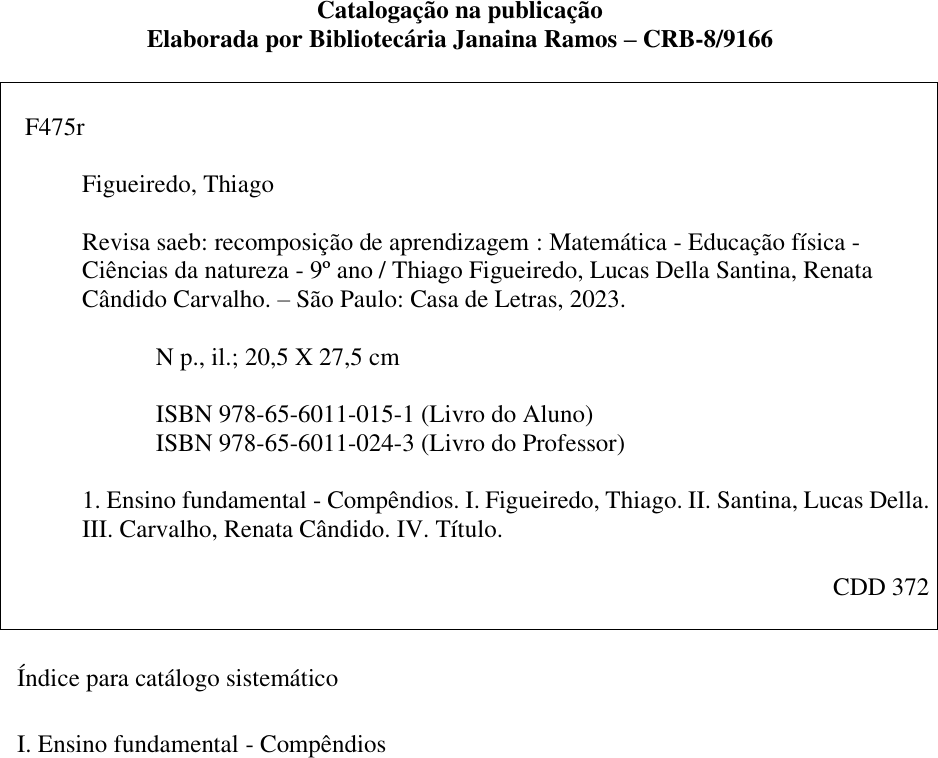
\includegraphics[width=.5\textwidth]{../fichas/9MAT.png}

\vfill

\textsc{casa de letras e gráfica ltda.}\\
Rua Fradique Coutinho, 1139, andar 2, sala 2\\
CEP 05416--011 -- São Paulo/\textsc{sp}, Brasil\\
Telefone: (11) 3914--7790\\\smallskip
www.casadeletras.com.br\\

\endgroup
\pagebreak
     % [Créditos]
% nothing			is level -3
% \book				is level -2
% \part				is level -1
% \chapter 			is level 0
% \section 			is level 1
% \subsection 		is level 2
% \subsubsection 	is level 3
% \paragraph 		is level 4
% \subparagraph 	is level 5
\setcounter{secnumdepth}{1}
\setcounter{tocdepth}{0}
 
% \renewcommand{\contentsname}{Índex} 	% Trocar nome do sumário para 'Índex'
%\ifodd\thepage\relax\else\blankpage\fi 	% Verifica se página é par e coloca página branca
%\tableofcontents*

\pagebreak
{\begingroup\mbox{}\pagestyle{empty}
\pagestyle{empty} 
% \renewcommand{\contentsname}{Índex} 	% Trocar nome do sumário para 'Índex'
%\ifodd\thepage\relax\else\blankpage\fi 	% Verifica se página é par e coloca página branca
\addtocontents{toc}{\protect\thispagestyle{empty}}
\tableofcontents*\clearpage\endgroup}


%!TEX root=./LIVRO.tex
\chapter{APRESENTAÇÃO}

O \textbf{SISTEMA DE AVALIAÇÃO DA EDUCAÇÃO BÁSICA (SAEB)} É UM CONJUNTO
DE AVALIAÇÕES EXTERNAS EM LARGA ESCALA QUE PERMITE AO INSTITUTO NACIONAL
DE ESTUDOS E PESQUISAS EDUCACIONAIS ANÍSIO TEIXEIRA (INEP) REALIZAR UM
DIAGNÓSTICO DA EDUCAÇÃO BÁSICA BRASILEIRA E DE FATORES QUE PODEM
INTERFERIR NO DESEMPENHO DOS ESTUDANTES.

POR MEIO DE TESTES E QUESTIONÁRIOS, APLICADOS A CADA DOIS ANOS NA REDE
PÚBLICA E EM UMA AMOSTRA DA REDE PRIVADA, O SAEB REFLETE OS NÍVEIS DE
APRENDIZAGEM DEMONSTRADOS PELOS ESTUDANTES AVALIADOS, EXPLICANDO ESSES
RESULTADOS A PARTIR DE UMA SÉRIE DE INFORMAÇÕES CONTEXTUAIS.

O SAEB PERMITE QUE AS ESCOLAS E AS REDES MUNICIPAIS E ESTADUAIS DE
ENSINO AVALIEM A QUALIDADE DA EDUCAÇÃO OFERECIDA AOS ESTUDANTES. O
RESULTADO DA AVALIAÇÃO É UM INDICATIVO DA QUALIDADE DO ENSINO BRASILEIRO
E OFERECE SUBSÍDIOS PARA ELABORAÇÃO, MONITORAMENTO E APRIMORAMENTO DE
POLÍTICAS EDUCACIONAIS, SEMPRE COM BASE EM EVIDÊNCIAS.

AS MÉDIAS DE DESEMPENHO DOS ESTUDANTES, APURADAS NO SAEB, JUNTAMENTE COM
AS TAXAS DE APROVAÇÃO, REPROVAÇÃO E ABANDONO, APURADAS NO CENSO ESCOLAR,
COMPÕEM O ÍNDICE DE DESENVOLVIMENTO DA EDUCAÇÃO BÁSICA (IDEB).

REALIZADO DESDE 1990, O SAEB PASSOU POR UMA SÉRIE DE APRIMORAMENTOS
TEÓRICO-METODOLÓGICOS AO LONGO DAS EDIÇÕES. A EDIÇÃO DE 2019 MARCA O
INÍCIO DE UM PERÍODO DE TRANSIÇÃO ENTRE AS MATRIZES DE REFERÊNCIA
UTILIZADAS DESDE 2001 E AS NOVAS MATRIZES ELABORADAS EM CONFORMIDADE COM
A BASE NACIONAL COMUM CURRICULAR (BNCC).

\section*{REVISA SAEB: REFORÇO ESCOLAR}

COMO O PRÓPRIO NOME DIZ, A EDUCAÇÃO BÁSICA É AQUELA EM QUE SE PROMOVE A
FORMAÇÃO MAIS ESSENCIAL DOS ALUNOS. O SISTEMA DE AVALIAÇÃO DA EDUCAÇÃO
BÁSICA (SAEB) AJUDA NA DETECÇÃO DOS PONTOS FORTES E FRACOS NA FORMAÇÃO
DOS ALUNOS EM ESTADOS, EM MUNICÍPIOS, EM ESCOLAS, FUNCIONANDO COMO UM
PARÂMETRO PARA QUE PROBLEMAS SEJAM SOLUCIONADOS E PARA QUE, ANO APÓS
ANO, ESSA FORMAÇÃO EVOLUA E AJUDE NO CRESCIMENTO DESSAS ESCOLAS, DESSES
MUNICÍPIOS E DESSES ESTADOS.

A PREPARAÇÃO ADEQUADA PARA AVALIAÇÕES EM LARGA ESCALA, COMO A DO SAEB, É
IMPORTANTE PARA QUE, NO MOMENTO DA PROVA, OS ALUNOS POSSAM ESTAR ATENTOS
E TRANQUILOS PARA DAREM O MELHOR POSSÍVEL DE SEU POTENCIAL. ASSIM, UM
MATERIAL DIDÁTICO DE APOIO QUE, DE FATO, PROMOVA ESSA PREPARAÇÃO É O
MAIOR DOS ALIADOS PARA PROFESSORES E GESTORES. ESTE MATERIAL TEM
EXATAMENTE ESTA INTENÇÃO: GARANTIR UM MELHOR APROVEITAMENTO DE CADA
ESTUDANTE NA RESOLUÇÃO DE ATIVIDADES, PARA QUE CONSIGAM RESULTADOS
EXCELENTES NESSA TRAJETÓRIA DE AVALIAÇÃO.

O \textbf{REVISA SAEB} ESTÁ DIVIDIDO EM 18 VOLUMES, DISTRIBUÍDOS, AO
LONGO DO ENSINO FUNDAMENTAL, DA SEGUINTE MANEIRA:

\begin{itemize}
\item
  NOS ANOS INICIAIS, PARA O \textbf{PRIMEIRO}, O \textbf{SEGUNDO}, O
  \textbf{TERCEIRO} E O \textbf{QUARTO ANO}, E NOS ANOS FINAIS, PARA O
  \textbf{SEXTO}, O \textbf{SÉTIMO} E O \textbf{OITAVO ANO}, EXISTE UM
  VOLUME POR ANO DE LÍNGUA PORTUGUESA E EXISTE UM VOLUME POR ANO DE
  MATEMÁTICA.
\item
  O \textbf{QUINTO ANO} APRESENTA UMA ESTRUTURA ESPECIAL. EM UM VOLUME,
  APARECEM ESTES COMPONENTES: LÍNGUA PORTUGUESA, ARTE E CIÊNCIAS
  HUMANAS. EM OUTRO VOLUME, APARECEM ESTES COMPONENTES: MATEMÁTICA,
  EDUCAÇÃO FÍSICA E CIÊNCIAS DA NATUREZA.
\item
  O \textbf{NONO ANO} TAMBÉM APRESENTA UMA ESTRUTURA ESPECIAL. SÃO DOIS
  VOLUMES: UM CONTÉM LÍNGUA PORTUGUESA, ARTE, LÍNGUA INGLESA E CIÊNCIAS
  HUMANAS; O OUTRO CONTÉM MATEMÁTICA, EDUCAÇÃO FÍSICA E CIÊNCIAS DA
  NATUREZA.
\end{itemize}

CADA VOLUME, EM CADA COMPONENTE, ESTÁ DIVIDIDO EM MÓDULOS TEMÁTICOS (DE
UMA OU DUAS AULAS), E CADA MÓDULO CONTA COM A ESTRUTURA DESCRITA A
SEGUIR.

\begin{itemize}
\item
  A \textbf{ABERTURA DO MÓDULO} APRESENTA UM RESUMO TEÓRICO DE
  CONTEXTUALIZAÇÃO, VINCULADO, PRINCIPALMENTE, A HABILIDADES DAS
  MATRIZES DO SAEB, MAS TAMBÉM A ALGUMAS HABILIDADES DA BNCC QUE TÊM
  RELAÇÃO COM ESSAS PRIMEIRAS HABILIDADES.
\item
  NA SEQUÊNCIA, ABRE-SE UMA SEÇÃO DE \textbf{ATIVIDADES}, QUE CONTÉM
  EXERCÍCIOS DE MODELOS VARIADOS PARA RETOMADA E FIXAÇÃO
  DO CONTEÚDO TRAZIDO PELO MÓDULO.
\item
  NO FECHAMENTO DE CADA MÓDULO, SURGE UMA SEÇÃO CHAMADA \textbf{TREINO},
  QUE CONTÉM TRÊS ITENS (QUESTÕES NO MODELO DO INEP, QUE É O MESMO
  UTILIZADO NOS TESTES COGNITIVOS DO SAEB). CADA ITEM CHECA O
  DESENVOLVIMENTO DE UMA HABILIDADE DAS MATRIZES DO SAEB E, SEMPRE QUE
  HÁ CONEXÃO, ESTÁ VINCULADO A UMA HABILIDADE DA BNCC DO ANO
  CORRESPONDENTE.
\item
  OS VOLUMES SE ENCERRAM COM QUATRO \textbf{SIMULADOS}, PARA SEREM
  APLICADOS BIMESTRALMENTE. AO LONGO DOS QUATROS SIMULADOS, TODAS AS
  HABILIDADES DAS MATRIZES DO SAEB, EM CADA ANO, SÃO TRABALHADAS, DESDE
  QUE VINCULADAS A CONTEÚDOS PREVISTOS PELA BNCC PARA O ANO EM
  ESPECÍFICO. IGUALMENTE COMPOSTOS DE ITENS, EM NÚMEROS VARIADOS, OS
  SIMULADOS TAMBÉM APRESENTAM, SEMPRE QUE HÁ CONEXÃO, HABILIDADES DA
  BNCC.
\end{itemize}

\addcontentsline{toc}{chapter}{Português}
\pagestyle{por}
\chapter[O alfabeto, as vogais e as consoantes]{\Large O alfabeto, as vogais e as consoantes}
\markboth{Módulo 1}{}

\colorsec{Habilidade do SAEB}

\begin{itemize}
\item Relacionar elementos sonoros das palavras com sua representação escrita.
\end{itemize}

\colorsec{Habilidade da BNCC}

\begin{itemize}
\item EF02LP03.
\end{itemize}

\conteudo{Para escrever as palavras, usamos as \textbf{letras}. 
Juntas, elas compõem o \textbf{alfabeto}, que é formado por 26 letras. 

As \textbf{vogais} são \textit{a, e, i, o, u}, e as outras letras são
chamadas de \textbf{consoantes}. Veja:

\begin{myquote}
b c d f g h j k l m n p q r s t v w x y z
\end{myquote}

Cada letra possui um nome e um som, que, quando estão juntos, podem
formar muitas palavras.

\begin{longtable}[]{@{}llllll@{}}
\toprule
\textbf{PATO} & \textbf{VACA} & \textbf{BOLA} & \textbf{TATU} &
\textbf{FADA} & \textbf{DOCE}\tabularnewline
\bottomrule
\end{longtable}

A letra C pode apresentar dois sons diferentes de acordo com a vogal que
acompanha. Por exemplo: junto com as vogais A, O e U, apresenta o som de 
/k/; junto com E e I apresenta o som de /s/.
}
 
%Felipe: precisamos padronizar como vamos grafar as letras e os fonemas, como ocorreu na frase acima. (Rogério, 13/3/23, 14h31)

\conteudo{
Algumas palavras com o som de /k/ também podem ser escritas com Q,
mas vale lembrar que o Q vem sempre acompanhado de U e de mais uma
vogal, e é esta última vogal que vai marcar o som da sílaba. Observe:

\begin{center}
\begin{tabular}{l}
\hline
\textbf{PALAVRAS C COM SOM DE /K/} \\ \hline
\textbf{CUCA} \\
\textbf{CASA} \\
\textbf{COCO} \\ \hline
\textbf{PALAVRAS C COM SOM DE /S/} \\ \hline
\textbf{CEBOLA} \\
\textbf{CINCO} \\
\textbf{CISNE} \\ \hline
\textbf{PALAVRAS COM QU} \\ \hline
\textbf{QUEIJO} \\
\textbf{QUILO} \\
\textbf{QUERO} \\
\textbf{QUIBE}
\end{tabular}
\end{center}

Veja a grafia dessas palavras.

\begin{myquote}
TATU \hspace{2cm}  GALO 
\end{myquote}

Na grafia das palavras com as vogais O e U, o O no final de palavras é
fraco, e o U é sempre forte.

\begin{quote}
A letra /k/ é usada apenas em situações como nomes de
pessoas, como Kátia, e palavras estrangeiras como
\textit{ketchup, kit, kibon} e \textit{kaiser}.
\end{quote}
}

\pagebreak
\colorsec{Atividades}

\num{1} Complete os nomes das figuras com as letras que estão faltando.

\begin{figure}[htpb!]

\includegraphics[width=.5\textwidth]{media/image1.jpeg}

\includegraphics[width=.5\textwidth]{media/image2.jpeg}
\end{figure}

T \reduline{A} P \reduline{E} T \reduline{E}\hspace{6cm} C \reduline{A} V \reduline{A} L \reduline{O}


\begin{figure}[htpb!]
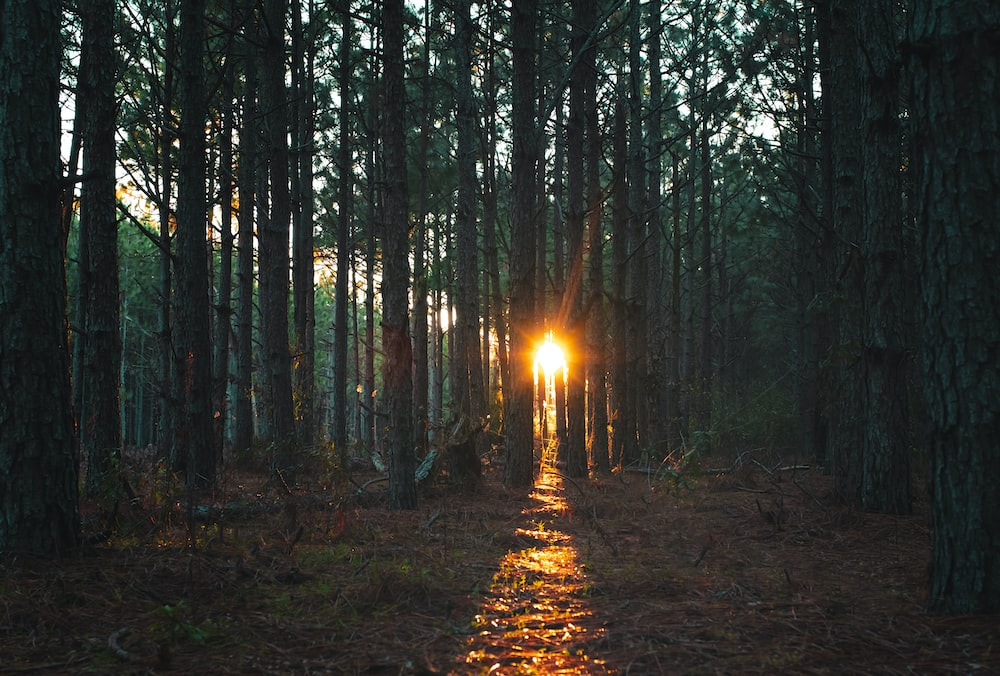
\includegraphics[width=.5\textwidth]{media/image3.jpeg}
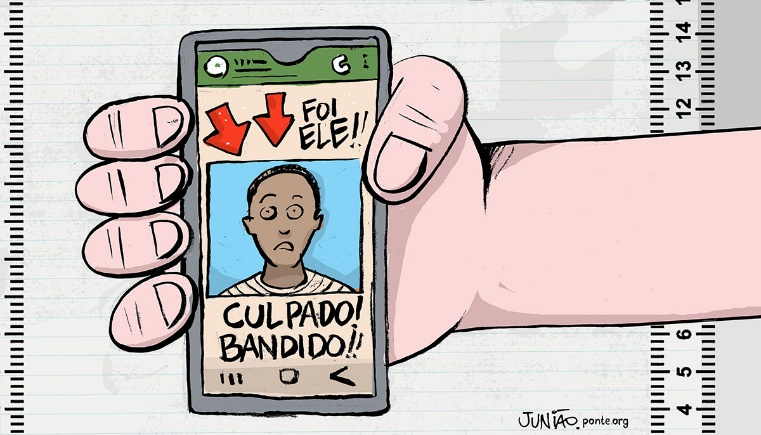
\includegraphics[width=.5\textwidth]{media/image4.jpeg}
\end{figure}

\reduline{E} STR \reduline{E} L \reduline{A} \hspace{6cm} P \reduline{O} RT \reduline{A}

\pagebreak
Você completou as palavras com

\begin{boxlist}
\boxitem{\white{X}} Vogais 

\boxitem{\white{X}} Consoantes
\end{boxlist}

%\coment{Apresente as vogais em cartaz. Pergunte o nome dos objetos representados nas imagens e, em seguida, convide as crianças para montar as palavras no alfabeto móvel para identificar as letras faltantes.}

\num{2} Complete o alfabeto com as letras que estão faltado.

\begin{center}
\Large
\begin{tabular}{|l|l|llllll}
\hline
\textbf{A} & \rosa{B} & \multicolumn{1}{l|}{\rosa{C}} & \multicolumn{1}{l|}{\rosa{D}} & \multicolumn{1}{l|}{\textbf{E}} & \multicolumn{1}{l|}{\rosa{F}} & \multicolumn{1}{l|}{\rosa{G}} & \multicolumn{1}{l|}{\rosa{H}} \\ \hline
\textbf{I} & \rosa{J} & \multicolumn{1}{l|}{\rosa{K}} & \multicolumn{1}{l|}{\rosa{L}} & \multicolumn{1}{l|}{\rosa{M}} & \multicolumn{1}{l|}{\rosa{N}} & \multicolumn{1}{l|}{\textbf{O}} & \multicolumn{1}{l|}{\rosa{P}} \\ \hline
\rosa{Q} & \rosa{R} & \multicolumn{1}{l|}{\rosa{S}} & \multicolumn{1}{l|}{\rosa{T}} & \multicolumn{1}{l|}{\textbf{U}} & \multicolumn{1}{l|}{\rosa{V}} & \multicolumn{1}{l|}{\rosa{W}} & \multicolumn{1}{l|}{\rosa{X}} \\ \hline
\rosa{Y} & \rosa{Z} & \textbf{} & \textbf{} & \textbf{} & \textbf{} & \textbf{} & \textbf{} \\ \cline{1-2}
\end{tabular}
\end{center}

Você completou as palavras com:

\begin{boxlist}
\boxitem{\white{X}} Vogais 

\boxitem{\white{X}} Consoantes
\end{boxlist}

%\coment{Leve o alfabeto móvel para sala e convide os alunos para organizar as letras na ordem certa. Em seguida, oriente-os a preencher o quadro; depois ajude a separar vogais e consoantes.}

\num{3} Leia o poema.

\textbf{A vaca Filomena e a formiga Violeta}



\includegraphics[width=.2\textwidth]{media/image5.jpeg}

\includegraphics[width=.3\textwidth]{media/image6.jpeg}

\begin{verse}
A vaca Filomena\\
mora na vila formosa.\\
A formiga Violeta\\
mora na cerca cor de rosa.

\pagebreak
A vaca Filomena\\
come as uvas da parreira.\\
A formiga Violeta\\
acha isto uma besteira.
\end{verse}

\fonte{Isabel Cristina Silveira Soares. https://seceducacao.padua.rj.gov.br/wp-content/uploads/2021/05/3o-ano-Ling.-Portuguesa-ATIV.17.pdf.
Acesso 28 de Fev 2023.}

Encontre e pinte no texto todas as palavras iniciadas com F e V. 
Depois escreva abaixo as palavras que encontrou.

\reduline{As palavras encontradas são as seguintes: vaca, Filomena, vila,
formosa, formiga, violeta.
Leve as palavras \textit{vaca} e \textit{formiga} em uma caixinha e
apresente-as para as crianças. Faça a leitura das palavras e estimule 
questionamentos sobre esses animais: os alunos sabem como eles são?
Onde esses animais vivem? Que sons eles emitem? Faça com os
alunos a leitura do poema e oriente a localização das palavras iniciadas
com as consoantes V e F.\hfill}

\num{4} Complete os espaços a seguir com as letras iniciais das palavras
\textit{violeta} e \textit{filomena}.

%\coment{Leve as palavras Violeta e Filomena em um cartaz. Explore a letra inicial e o som da letra nas palavras.}

\begin{figure}[htpb!]

\includegraphics[width=.3\textwidth]{media/image7.jpeg}

\includegraphics[width=.3\textwidth]{media/image8.jpeg}

\includegraphics[width=.3\textwidth]{media/image9.jpeg}
\end{figure}

\reduline{F} ACA \hspace{4cm} \reduline{F} ADA \hspace{3cm} \reduline{V} ELA

\pagebreak
\begin{figure}[htpb!]

\includegraphics[width=.3\textwidth]{media/image10.jpeg}
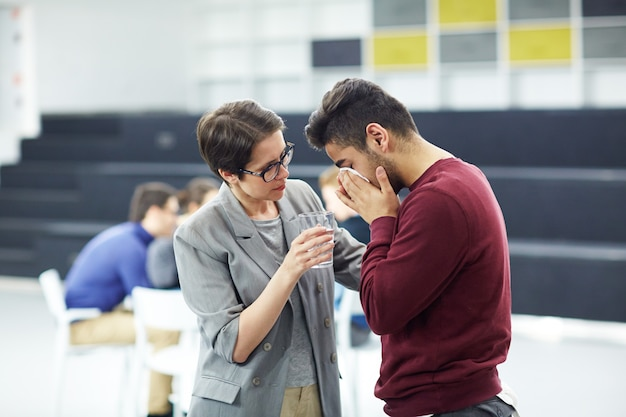
\includegraphics[width=.3\textwidth]{media/image11.jpeg}

\includegraphics[width=.3\textwidth]{media/image12.jpeg}
\end{figure}

 \reduline{V} ASSOURA \hspace{4cm} \reduline{F} OGO \hspace{3cm} \reduline{F} IVELA

\begin{figure}[htpb!]
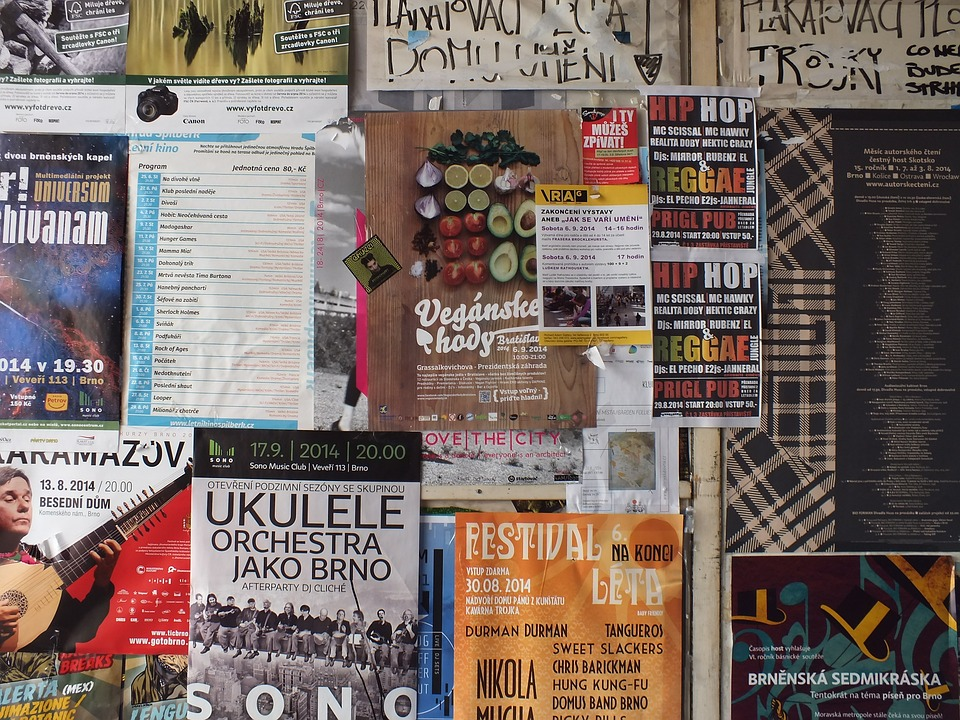
\includegraphics[width=.3\textwidth]{media/image13.jpeg}

\includegraphics[width=.3\textwidth]{media/image14.jpeg}

\includegraphics[width=.3\textwidth]{media/image15.jpeg}
\end{figure}

\reduline{F} LOR \hspace{4cm} \reduline{F} OGUETE \hspace{3cm} SOR \reduline{V} ETE


\num{5} Pinte as iniciais de cada palavra.

%\coment{Leve para sala palavras iniciadas pelas letras T, D, F, V, B, P. Convide as crianças para fazer a leitura, identificado o som das letras iniciais e finais, e quantidade de sílabas. Também é possível trabalhar a função social da escrita das palavras}.

\begin{center}
\begin{tabular}{|c|c|c|c|c|}
\hline
\textbf{VACINA} & F & T & D & \rosa{V} \\ \hline
\textbf{TESOURA} & P & D & \rosa{T} & F \\ \hline
\textbf{VASSOURA} & B & T & \rosa{V} & F \\ \hline
\textbf{FACA} & V & \rosa{F} & D & T \\ \hline
\textbf{DEDO} & T & V & F & \rosa{D} \\ \hline
\textbf{PANELA} & V & T & \rosa{P} & B \\ \hline
\textbf{DOMINÓ} & B & \rosa{D} & T & P \\ \hline
\textbf{BONECA} & F & P & \rosa{B} & D \\ \hline
\end{tabular}
\end{center}

\pagebreak
\num{6} Numere os desenhos conforme os números das palavras.

%\coment{Faça leitura das palavras com as crianças, de modo que elas identifiquem a numeração e façam a associação correta.}

\begin{multicols}{3}
\begin{enumerate}
\item BOLA

\item FOCA

\item TATU

\item PANELA

\item TAPETE

\item FORMIGA

\item DADO

\item VACA

\item PATO

\item BONECA
\end{enumerate}
\end{multicols}

\begin{longtable}[]{@{}llll@{}}
\reduline{\_\_10\_\_} &
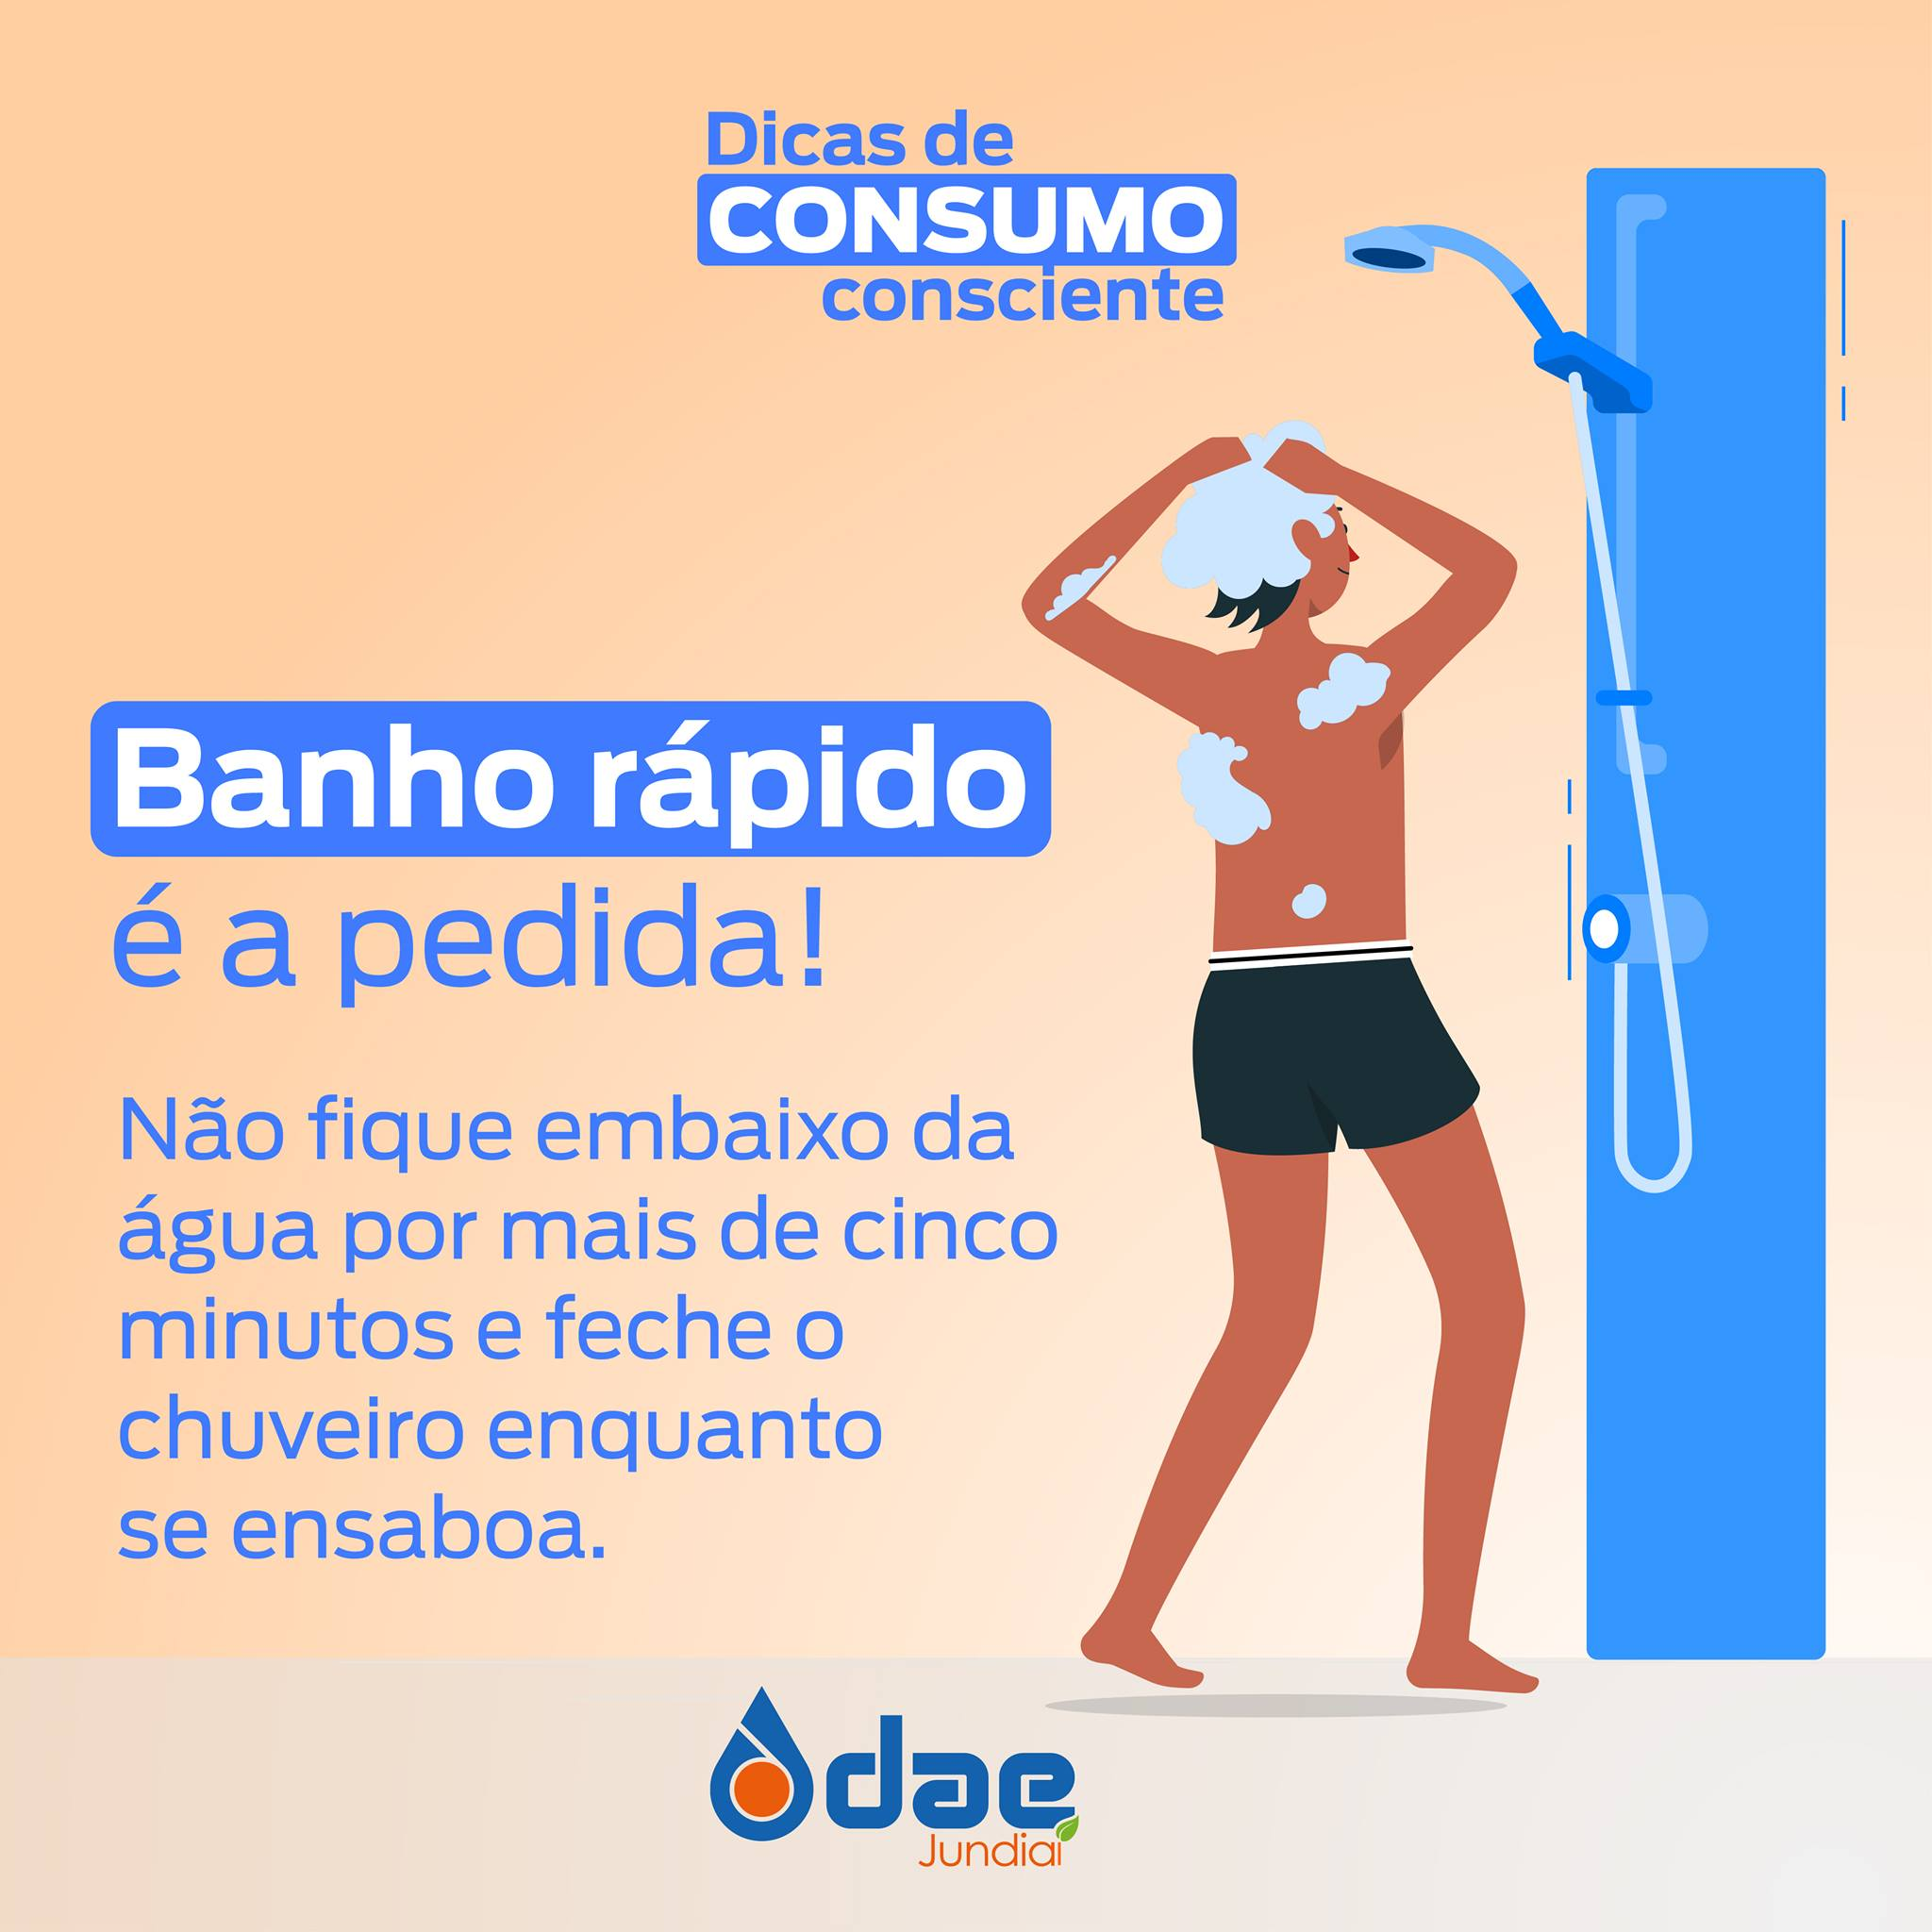
\includegraphics[width=1.16667in,height=0.96319in]{media/image16.jpeg} &
\reduline{\_\_8\_\_} &
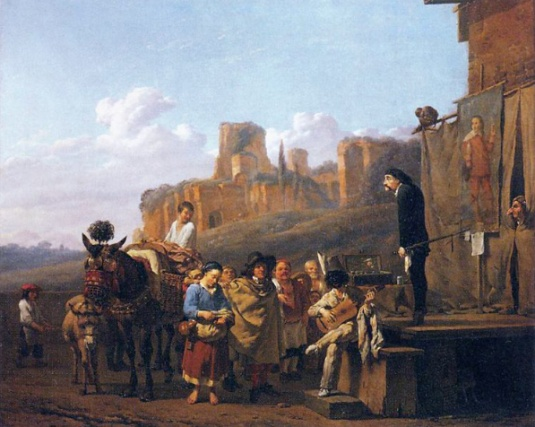
\includegraphics[width=1.16127in,height=0.95833in]{media/image17.jpeg}\tabularnewline
\reduline{\_\_2\_\_} &

\includegraphics[width=1.09375in,height=1.09375in]{media/image18.jpeg} &
\reduline{\_\_4\_\_} &
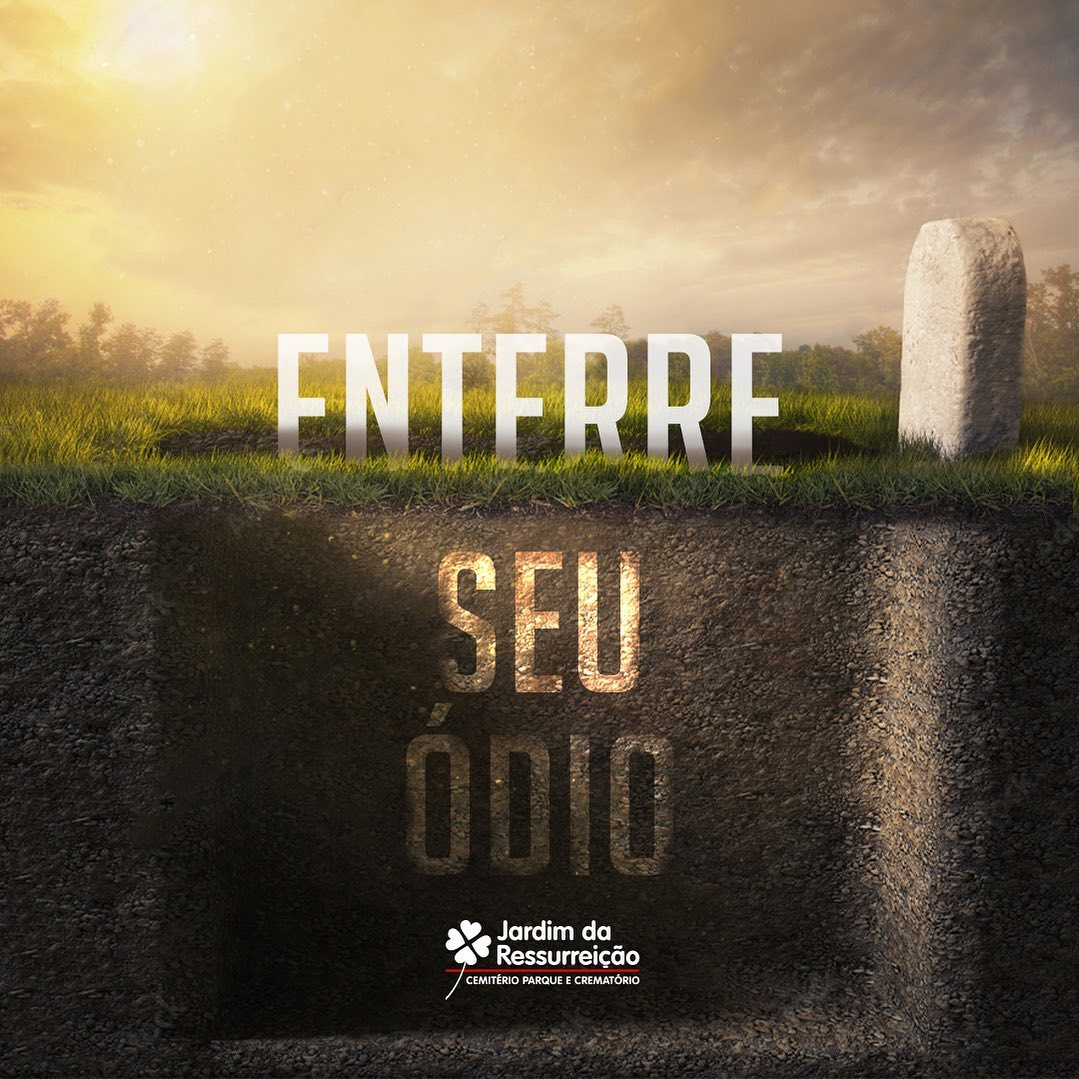
\includegraphics[width=1.27986in,height=0.98958in]{media/image19.jpeg}\tabularnewline
\reduline{\_\_3\_\_} &

\includegraphics[width=0.92708in,height=0.92708in]{media/image20.jpeg} &
\reduline{\_\_6\_\_} &
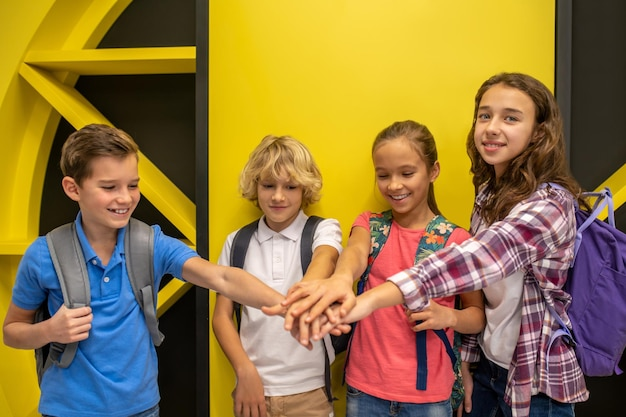
\includegraphics[width=0.97986in,height=1.05208in]{media/image21.jpeg}\tabularnewline
\reduline{\_\_1\_\_} &
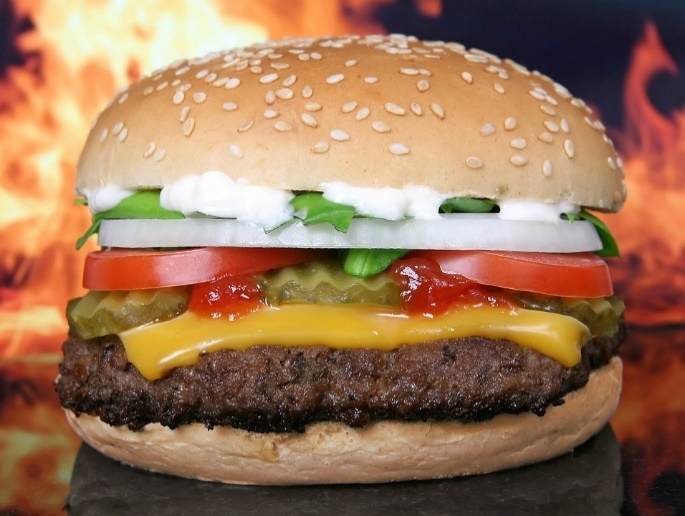
\includegraphics[width=1.13542in,height=1.13542in]{media/image22.jpeg} &
\reduline{\_\_7\_\_} &
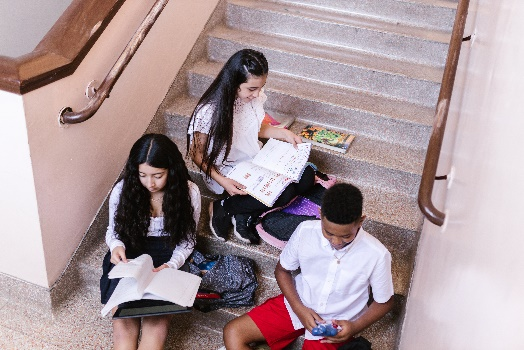
\includegraphics[width=1.23958in,height=1.15833in]{media/image23.jpeg}\tabularnewline
\reduline{\_\_9\_\_} &

\includegraphics[width=1.19722in,height=1.27083in]{media/image24.jpeg} &
\reduline{\_\_5\_\_} &

\includegraphics[width=2.21875in,height=1.11458in]{media/image25.jpeg}\tabularnewline
\end{longtable}

\pagebreak
\num{7} Complete as palvaras com \textbf{-ca -co -cu} ou \textbf{-qua -que -qui}.

%\coment{Convide as crianças a falar o nome das imagens para identificar a grafia da palavra.}

\begin{figure}[htpb!]

\includegraphics[width=.24\textwidth]{media/image26.jpeg}
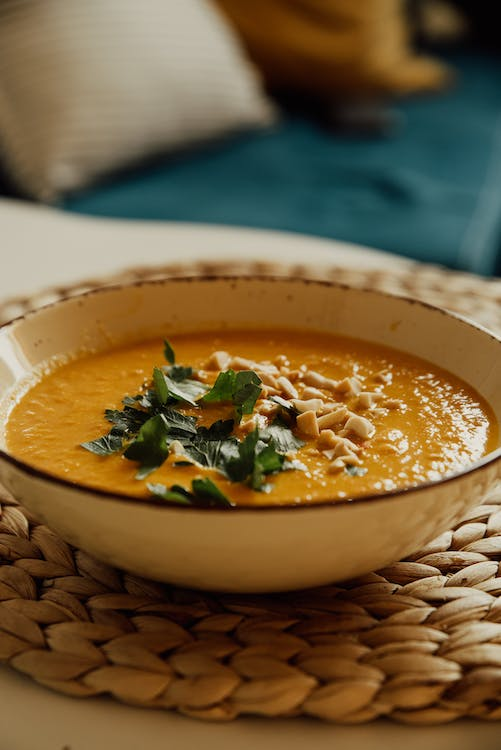
\includegraphics[width=.24\textwidth]{media/image27.jpeg}
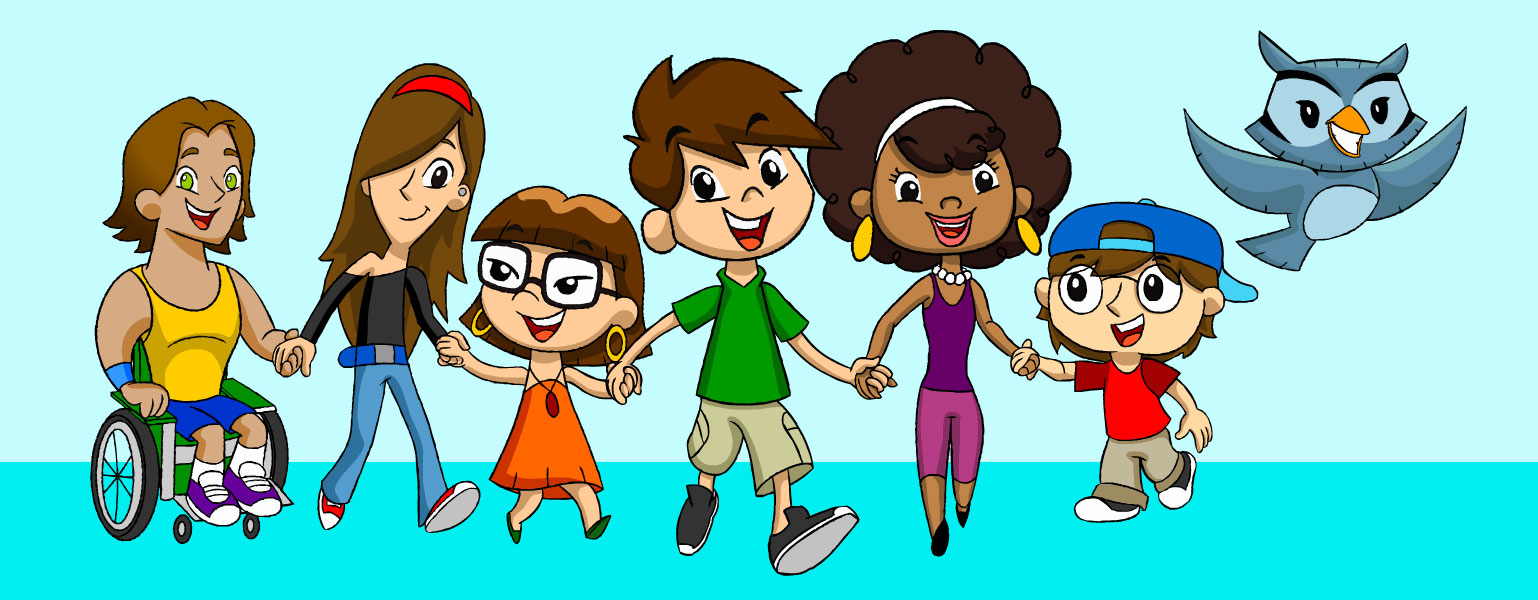
\includegraphics[width=.24\textwidth]{media/image28.jpeg}
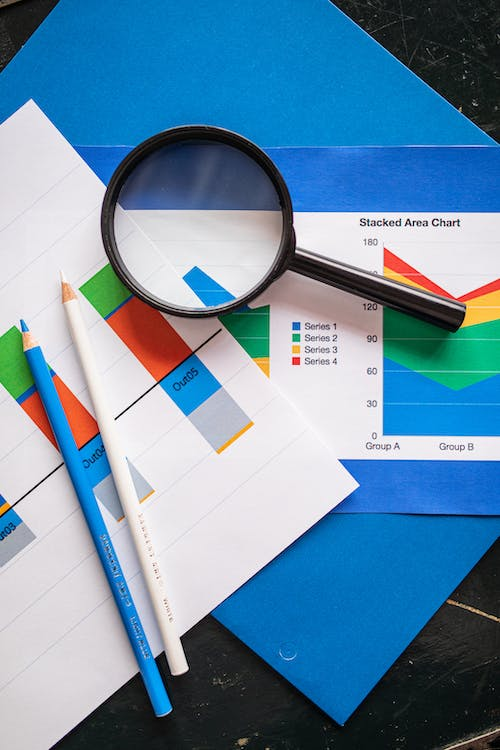
\includegraphics[width=.24\textwidth]{media/image29.jpeg}
\end{figure}

\reduline{CU} TIA \hspace{2cm} \reduline{CA} SA \hspace{2cm} \reduline{CU} SCUZ \hspace{2cm} \reduline{QUE} IJO

\begin{figure}[htpb!]
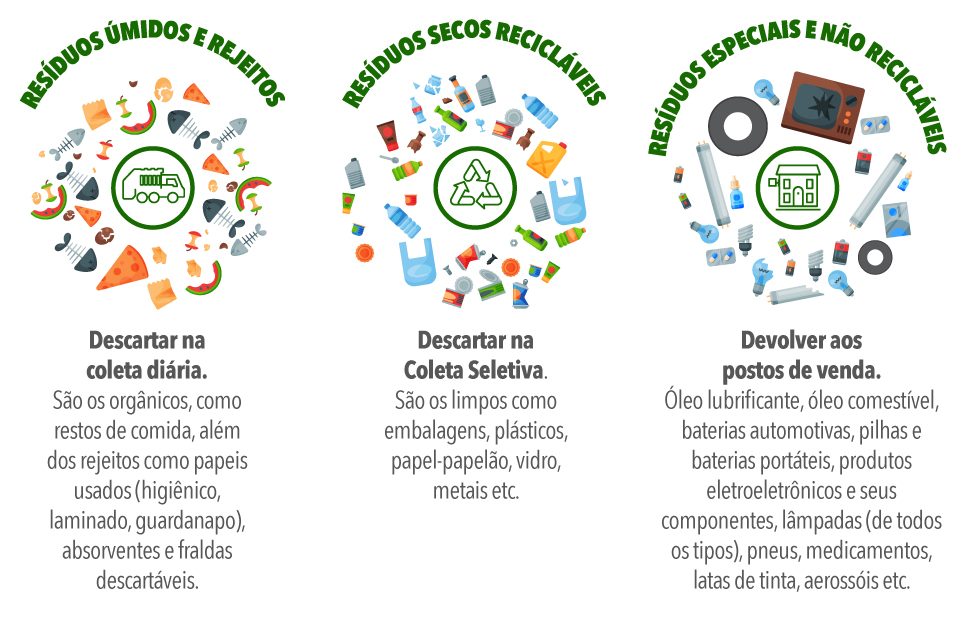
\includegraphics[width=.24\textwidth]{media/image30.jpeg}

\includegraphics[width=.24\textwidth]{media/image31.jpeg}
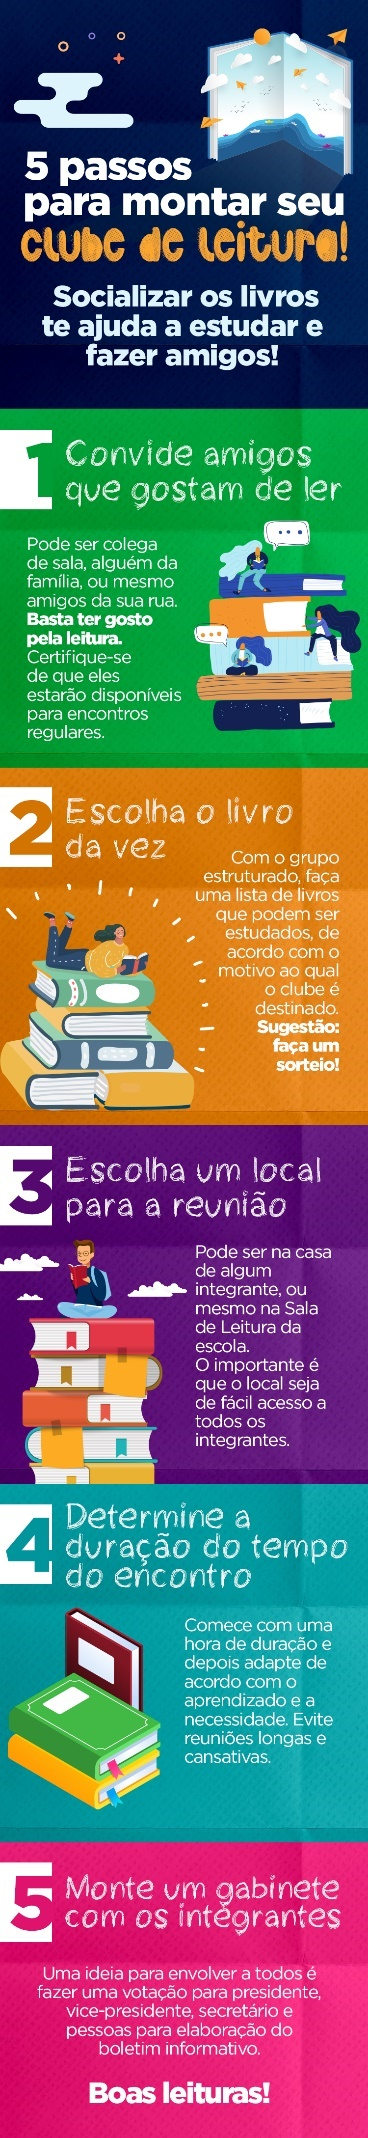
\includegraphics[width=.24\textwidth]{media/image32.jpeg}
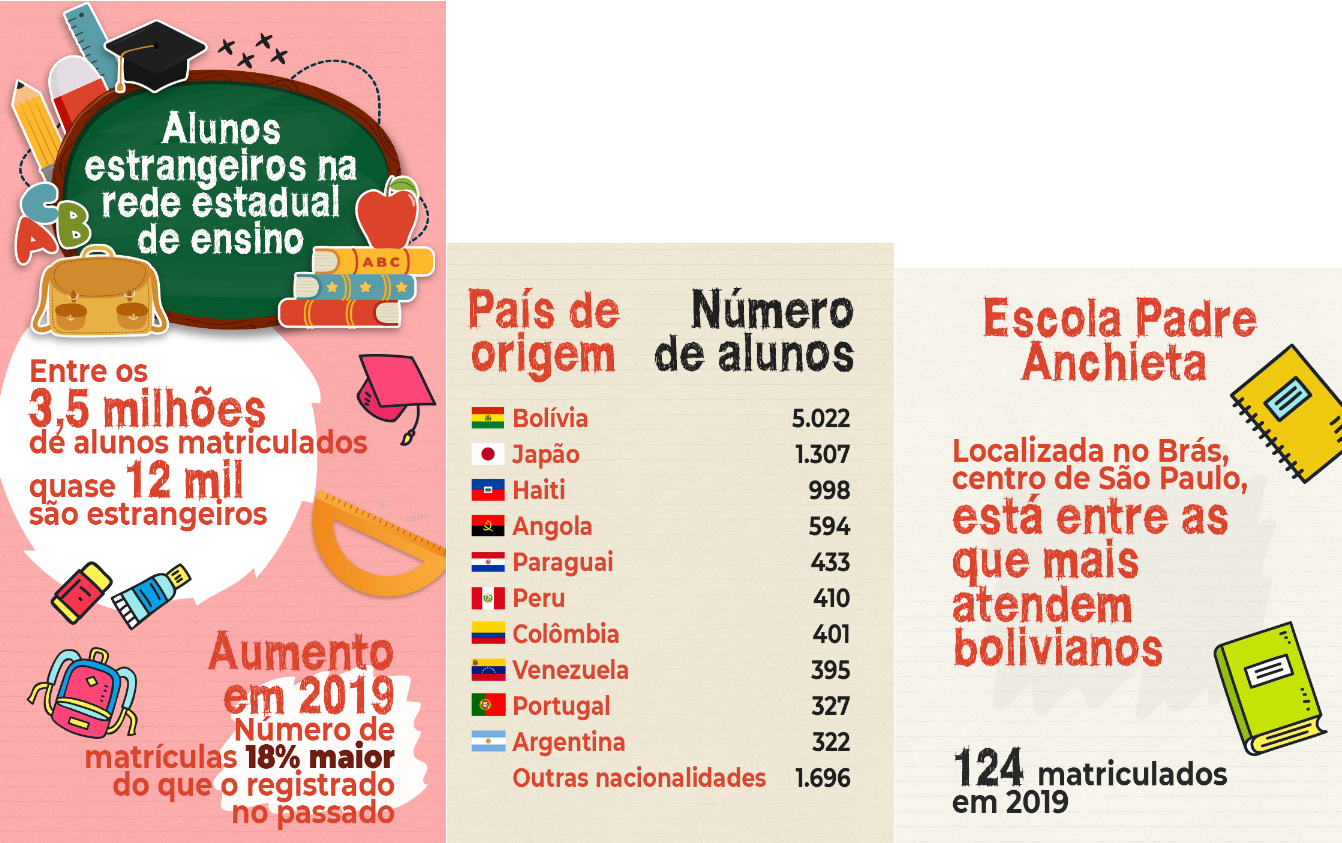
\includegraphics[width=.24\textwidth]{media/image33.jpeg}
\end{figure}

A \reduline{QUÁ} RIO \hspace{1cm} \reduline{QUI} NZE \hspace{1cm} RA \reduline{QUE} TE \hspace{1cm} \reduline{CO} LA


\num{8} Encontre a sílaba mais forte e complete com O ou U.

%\coment{Leve para a classe uma caixinha enfeitada com palavras terminadas com O e U. Passe a caixinha para os alunos em círculo, ao som de uma música. Quando a música parar, o aluno que estiver com a caixinha na mão deve ler a palavra observando a letra  final. Em seguida, convide toda a turma a pronunciar a palavra e, então, descobrir a sílaba forte. Explique como descobrir quando a sílaba é forte e fraca, ensinando que, quando o U está no final, ele é sempre forte, e que o O é sempre fraco no final das palavras.}

\begin{figure}[htpb!]

\includegraphics[width=.3\textwidth]{media/image34.jpeg}

\includegraphics[width=.3\textwidth]{media/image35.jpeg}
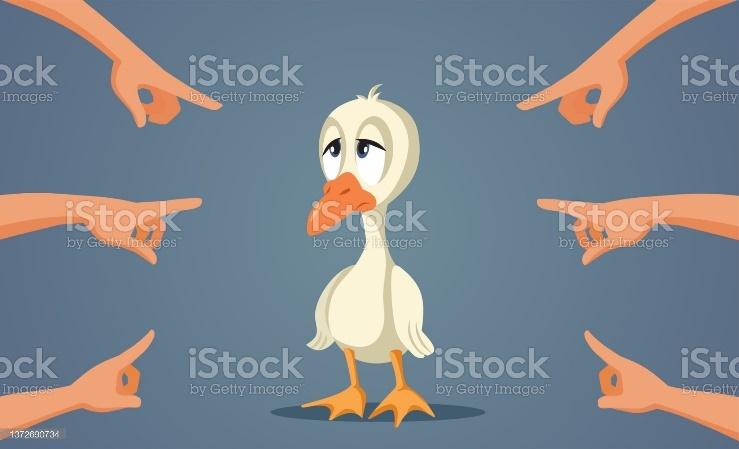
\includegraphics[width=.2\textwidth]{media/image36.jpeg}
\end{figure}

SAPAT \reduline{O} \hspace{3cm} VAS \reduline{O} \hspace{2cm} TAT \reduline{U}

\begin{figure}[htpb!]
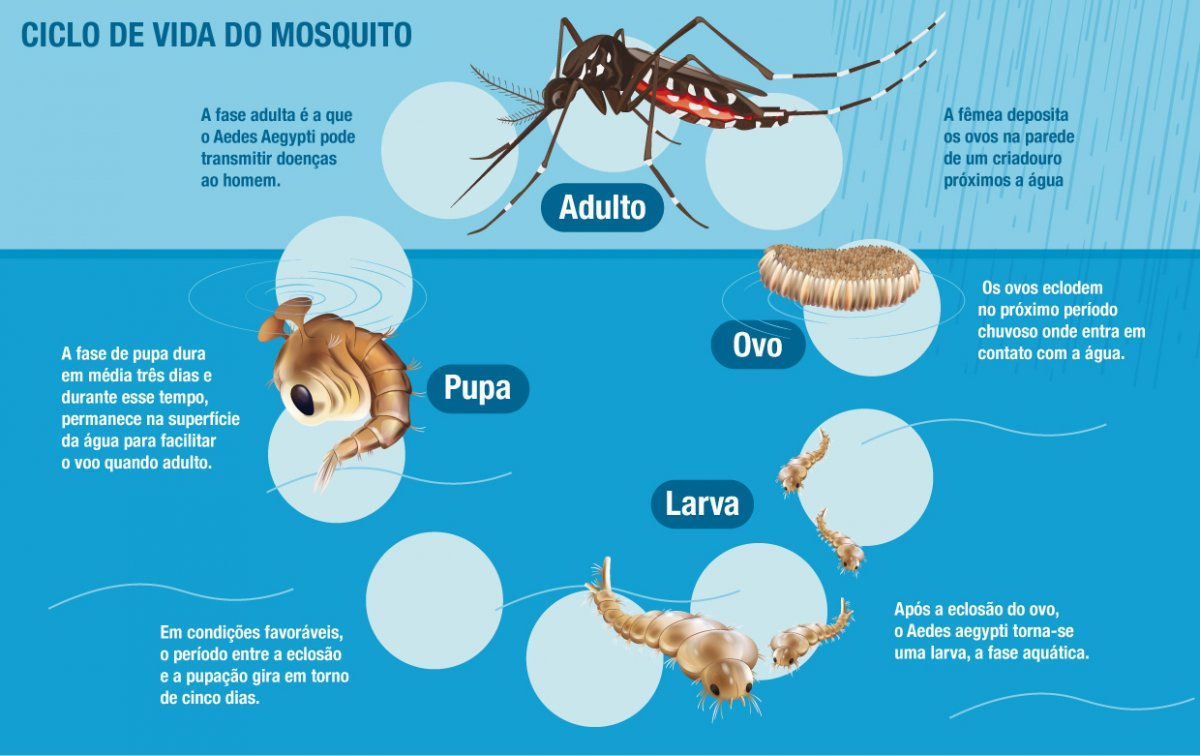
\includegraphics[width=.2\textwidth]{media/image37.jpeg}
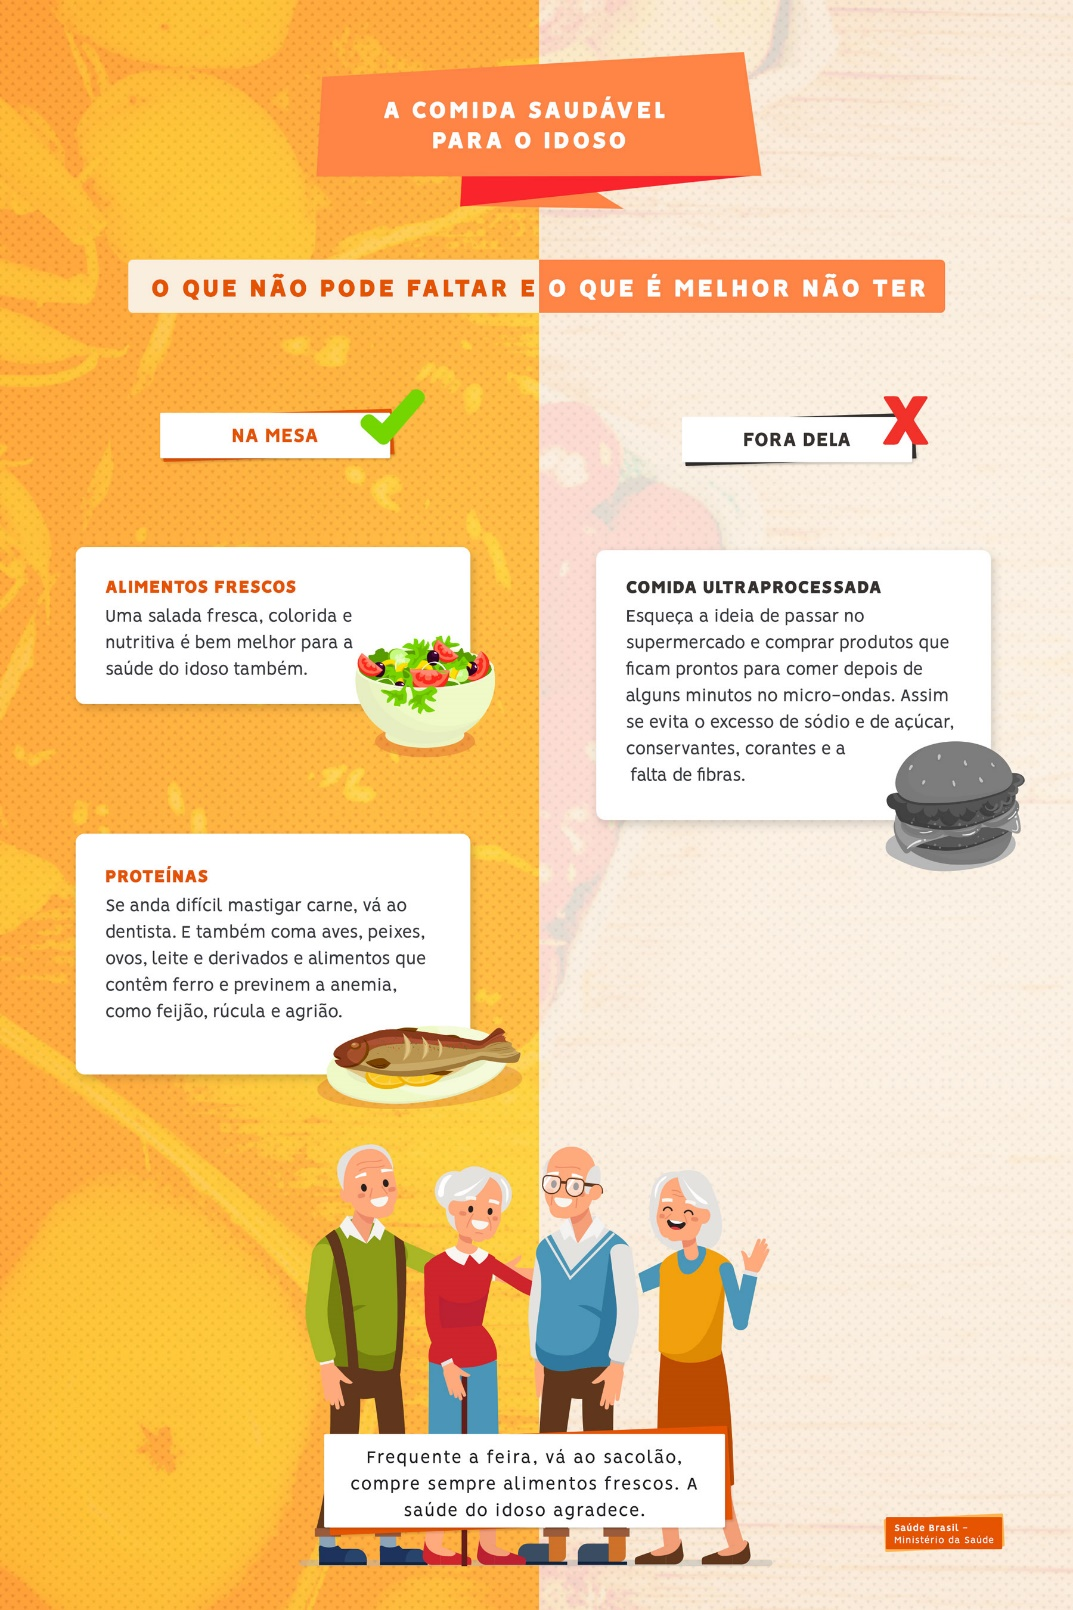
\includegraphics[width=.3\textwidth]{media/image38.jpeg}

\includegraphics[width=.2\textwidth]{media/image39.jpeg}
\end{figure}

ESPELH \reduline{O} \hspace{1cm} CAJ \reduline{U} \hspace{2cm} CABEL \reduline{O}


\num{9} Pinte as palvras escritas com C que tem o som de S.
%Felipe: aqui precisamos padronizar, como comentei anteriormente. 

%\coment{Leve para sala palavras escritas com C. Organize uma roda de conversa na qual você orientará os alunos a organizar as palavras de acordo com a vogal que acompanha a letra C. Em seguida, explique a regra para descobrir se o C tem som de K ou S.}

\begin{longtable}[]{@{}lllll@{}}
\toprule
\textbf{CINEMA} & \textbf{CASA} & \textbf{CISNE} & \textbf{CEGO} &
\textbf{COCADA}\tabularnewline
\midrule
\endhead
\textbf{CADEIRA} & \textbf{CARRO} & \textbf{CINTO } & \textbf{COCO} &
\textbf{CAMA}\tabularnewline
\bottomrule
\end{longtable}

\num{10} Troque as letras e forme outras palavras.

%\coment{Utilize o alfabeto móvel com as palavras solicitadas no exercício e outras. Também é possível fazer a brincadeira da forca.}

\begin{longtable}[]{@{}lll@{}}
\toprule
\textbf{V POR F} & \textbf{D POR T} & \textbf{B POR P}\tabularnewline
\midrule
\endhead
\textbf{VACA} & \textbf{DADO} & \textbf{BODE}\tabularnewline
\textbf{\reduline{F}ACA} & \textbf{\reduline{T}ATO} & \textbf{\reduline{P}ODE}\tabularnewline
\textbf{VILA} & \textbf{DIA} & \textbf{BOTE}\tabularnewline
\textbf{\reduline{F}I LA} & \textbf{\reduline{T}IA} & \textbf{\reduline{P}OTE}\tabularnewline
\bottomrule
\end{longtable}

\pagebreak
\num{11} Complete a cruzadinha com o nome das figuras.

%\coment{Explore as frutas e legumes da atividade, fazendo questionamentos. Monte as palavras no alfabeto móvel com as crianças. Em seguida, oriente a escrita na cruzadinha.}

\begin{figure}[htpb!]

\includegraphics[width=\textwidth]{media/image40.png}
\end{figure}

\num{12} Encontre e pinte as palavras no diagrama.

%\coment{Depois da leitura das palavras, oriente os alunos a localizá-las no diagrama.}

\begin{longtable}[]{@{}llllllll@{}}
\toprule
	TATU -- CABELO -- BONECA -- PANELA -- CAJU\tabularnewline
FADA -- DADO -- VASO -- CAMA -- TAPETE\tabularnewline
\midrule
D & B & F & A & D & A & D & G\tabularnewline
A & C & A & B & E & L & O & U\tabularnewline
G & Y & B & O & C & A & M & A\tabularnewline
S & T & I & N & H & M & A & Q\tabularnewline
P & A & N & E & L & A & D & F\tabularnewline
H & T & O & C & A & J & U & L\tabularnewline
J & U & K & A & D & A & D & O\tabularnewline
T & A & P & E & T & E & Z & X\tabularnewline
K & V & A & S & O & B & G & J\tabularnewline
\end{longtable}

\pagebreak
\colorsec{Treino}

\num{1} Observe o animal que Júlia encontrou enquanto brincava na 
fazenda do Tio Belo.

\begin{figure}[htpb!]
\centering

\includegraphics[width=.9\textwidth]{media/image42.jpeg}
\end{figure}

A palavra que começa com a mesma letra do nome do animal que Júlia encontrou é

\begin{escolha}
\item vaso.

\item gato.

\item bola.

\item foca
\end{escolha}


\num{2} Observe a palavra que Tiago leu para sua professora.

\begin{myquote}
CAJU
\end{myquote}

O nome da figura que termina com a mesma letra da palavra que Tiago leu é

\begin{escolha}
\item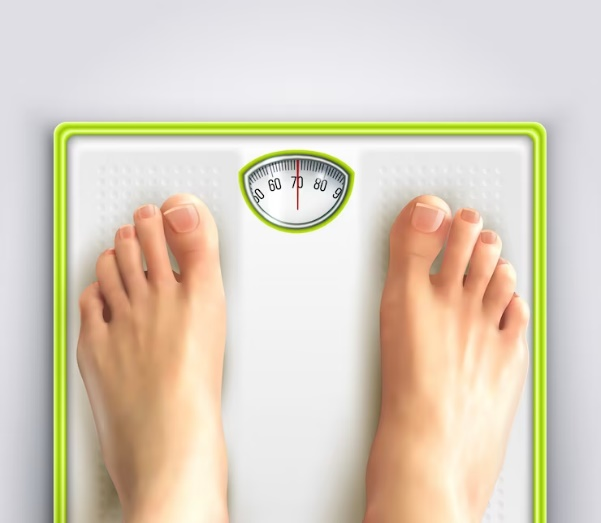
\includegraphics[width=0.79792in,height=0.81667in]{media/image44.jpeg}

\item
\includegraphics[width=1.02847in,height=0.72292in]{media/image45.jpeg}

\item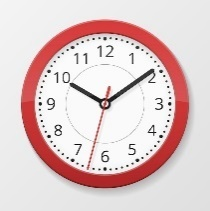
\includegraphics[width=0.79792in,height=0.79931in]{media/image46.jpeg}

\item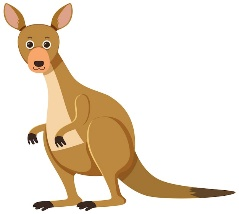
\includegraphics[width=1.08611in,height=0.97222in]{media/image47.jpeg}
\end{escolha}


\num{3} Observe o presente que Bruna ganhou.

\begin{figure}[htpb!]
\centering
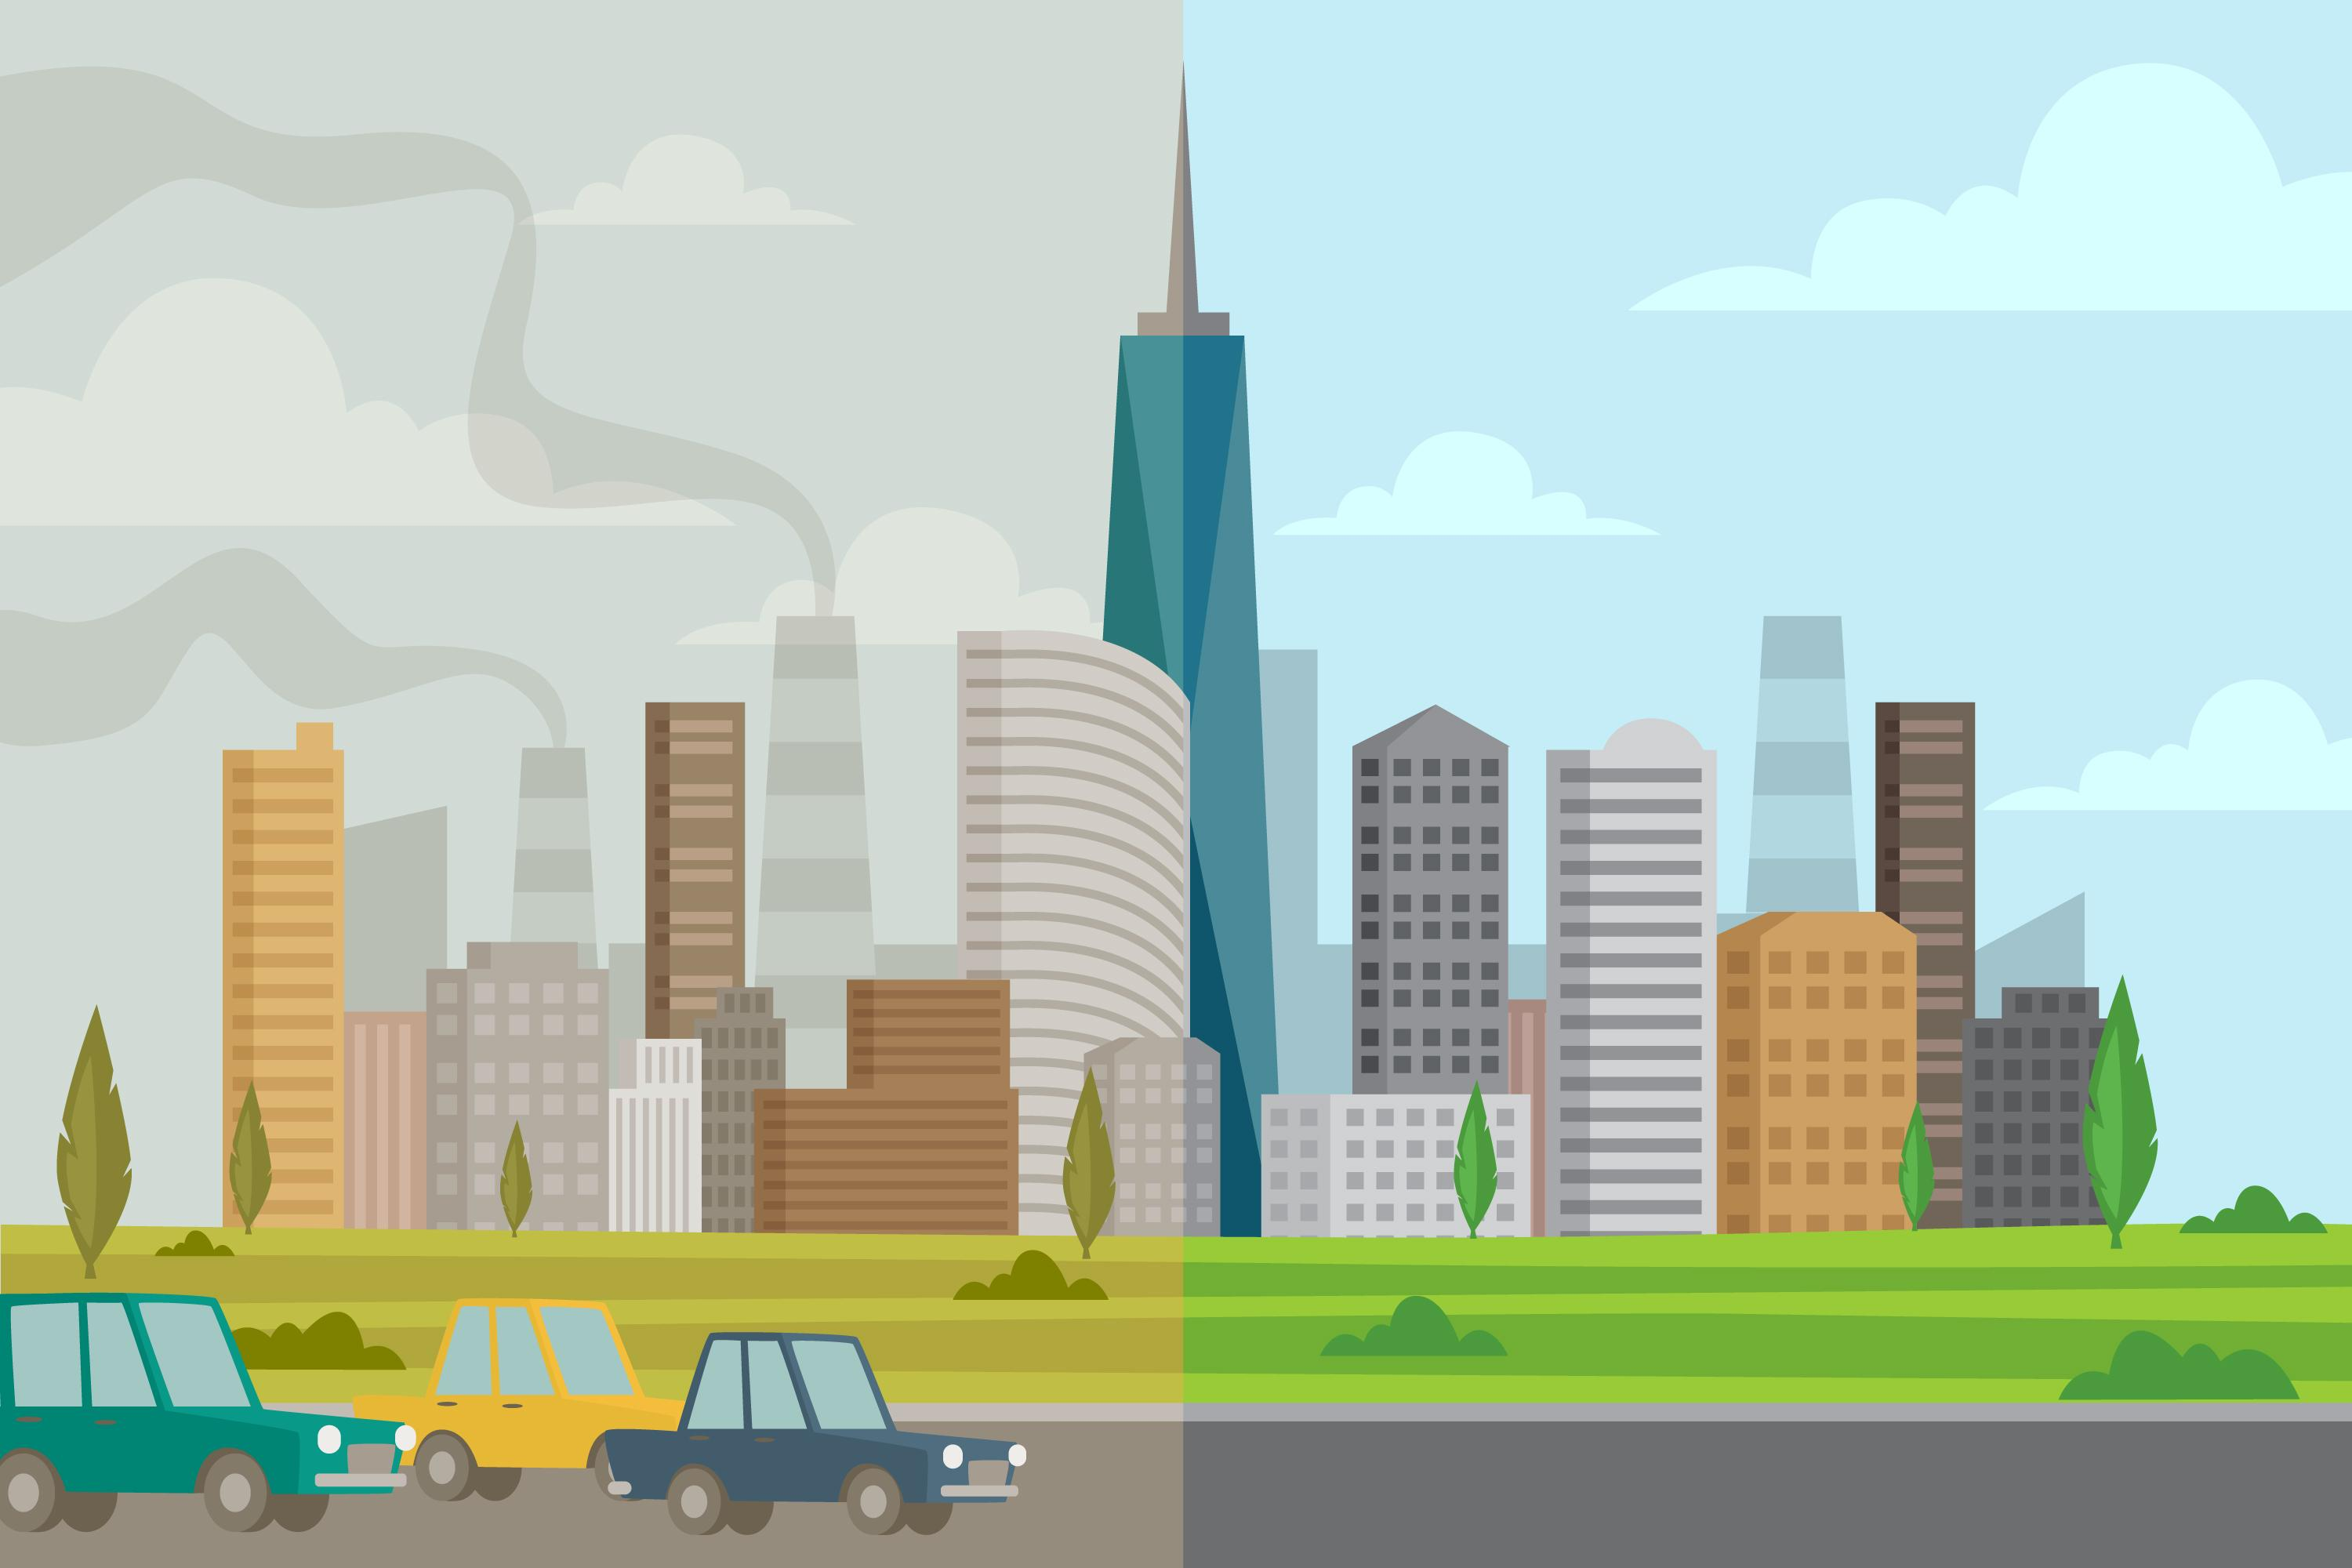
\includegraphics[width=.3\textwidth]{media/image48.jpeg}
\end{figure}

A palavra que começa como o mesmo som da letra do nome do presente de Bruna é

\begin{multicols}{2}
\begin{escolha}
\item cama.

\item cubo.

\item cebola.

\item cocada.
\end{escolha}
\end{multicols}

\chapter{Lendo e escrevendo}
\markboth{Módulo 2}{}

\vspace*{-1.5cm}

\colorsec{Habilidades do SAEB}

\begin{itemize}
\item Ler palavras.
\item Escrever palavras.
\item Ler frases.
\end{itemize}

\colorsec{Habilidades da BNCC}

\begin{itemize}
\item EF02LP04, EF02LP05.
\end{itemize}

\conteudo{Para escrever uma palavra, você precisa usar as letras que
são chamadas de vogais e as consoantes.

As vogais são 

\begin{myquote}
\textbf{A -- E -- I -- O -- U} 
\end{myquote}

e as consoantes são

\begin{myquote}
\textbf{B -- C -- D -- F -- G -- H -- J -- K -- L -- M -- N -- P -- Q -- R -- S
-- T -- V -- W -- Y -- X -- Z.}
\end{myquote}

As palavras são lidas e escritas da esquerda para a direita.

\begin{myquote}
$\longrightarrow$

\textbf{GRAVIOLA LÂMPADA AVIÃO LARANJA }
\end{myquote}

Existem diferentes maneiras de compor a sílaba de uma palavra. 

\textbf{CONSOANTE + VOGAL}: é o que acontece nas três sílabas das 
palavras \textit{sapato} e \textit{telefone}: SA-PA-TO e TE-LE-FO-NE

\textbf{VOGAL}: é o que acontece na segunda sílaba das  
palavras \textit{saída} e \textit{saúde}: SA-Í-DA e SA-Ú-DE

\textbf{CONSOANTE + VOGAL + CONSOANTE}: é o que acontece na 
primera sílaba das palavras \textit{porta} e \textit{cortina}:
POR-TA e COR-TI-NA

\textbf{CONSOANTE + CONSOANTE + VOGAL}: é o que acontece na 
primera sílaba da palavra \textit{criança} e na última
sílaba da palavra \textit{livro}: CRI-AN-ÇA e LI-VRO 

Observe o quadro abaixo, com outros exemplos:\bigskip

\noindent{\tiny
\begin{tabular}{l|l|l|l|l|}
\cline{2-5}
 & \textbf{GRAVIOLA} & \textbf{LÂMPADA} & \textbf{AVIÃO} & \textbf{LARANJA} \\ \hline
\multicolumn{1}{|l|}{\textbf{FORMAÇÃO SILÁBICA CV}} & GRA - \textbf{VI} - O - \textbf{LA} & LÂM - \textbf{PA} - \textbf{DA} & A - \textbf{VI} -ÃO & \textbf{LA} - RAN - \textbf{JA} \\ \hline
\multicolumn{1}{|l|}{\textbf{FORMAÇÃO SILÁBICA V}} & GRA - VI - \textbf{O} - LA & \multicolumn{1}{c|}{*} & \textbf{A} - VI -ÃO & \multicolumn{1}{c|}{*} \\ \hline
\multicolumn{1}{|l|}{\textbf{FORMAÇÃO SILÁBICA CVC}} & \multicolumn{1}{c|}{*} & \textbf{LÂM} - PA - DA & \multicolumn{1}{c|}{*} & LA - \textbf{RAN} - JA \\ \hline
\multicolumn{1}{|l|}{\textbf{FORMAÇÃO SILÁBICA CCV}} & \textbf{GRA} - VI - O - LA & \multicolumn{1}{c|}{*} & \multicolumn{1}{c|}{*} & \multicolumn{1}{c|}{*} \\ \hline
\end{tabular}
}


Note que, em todas as formações das sílabas, aparecem vogais. Isso
acontece porque não existe sílaba sem vogal, isto é, uma  sílaba não
se forma só com consoantes.

Observe a frase a seguir:

\begin{myquote}
\textbf{O avião pousou cedo.}
\end{myquote}

Você conhece esse sinal em cima da letra A da palavra \textbf{avião}?

Esse sinal é o \textbf{til}, usado nas vogais A e O para marcar a
nasalidade presente na sílaba.

As marcas de nasalidade aparece também nas letras M e N, no final da
sílaba. É o que acontece, por exemplo, com as seguintes palavras:

\begin{myquote}
\textbf{LÂMPADA E LARANJA}
\end{myquote}

A letra \textbf{M} é utilizada antes das consoantes P e B.  
A letra \textbf{N} é usada antes das demais consoantes, nunca 
no final das palavras.
}

\colorsec{Atividades}

\num{1} Escreva os nomes das figuras.

%\coment{Leve o alfabeto móvel para a sala de aula. Convide as crianças para manusear as letras; em seguida, oriente-as a formar as palavras que nomeiam as figuras. Sugira a elas que, antes de escrever, elas devem pronunciar a palavra, escrevendo-a por sílabas ou pedacinhos.}


\begin{figure}[htpb!]
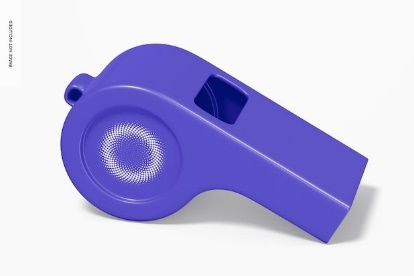
\includegraphics[width=1.46154in,height=0.93603in]{media/image49.jpeg}
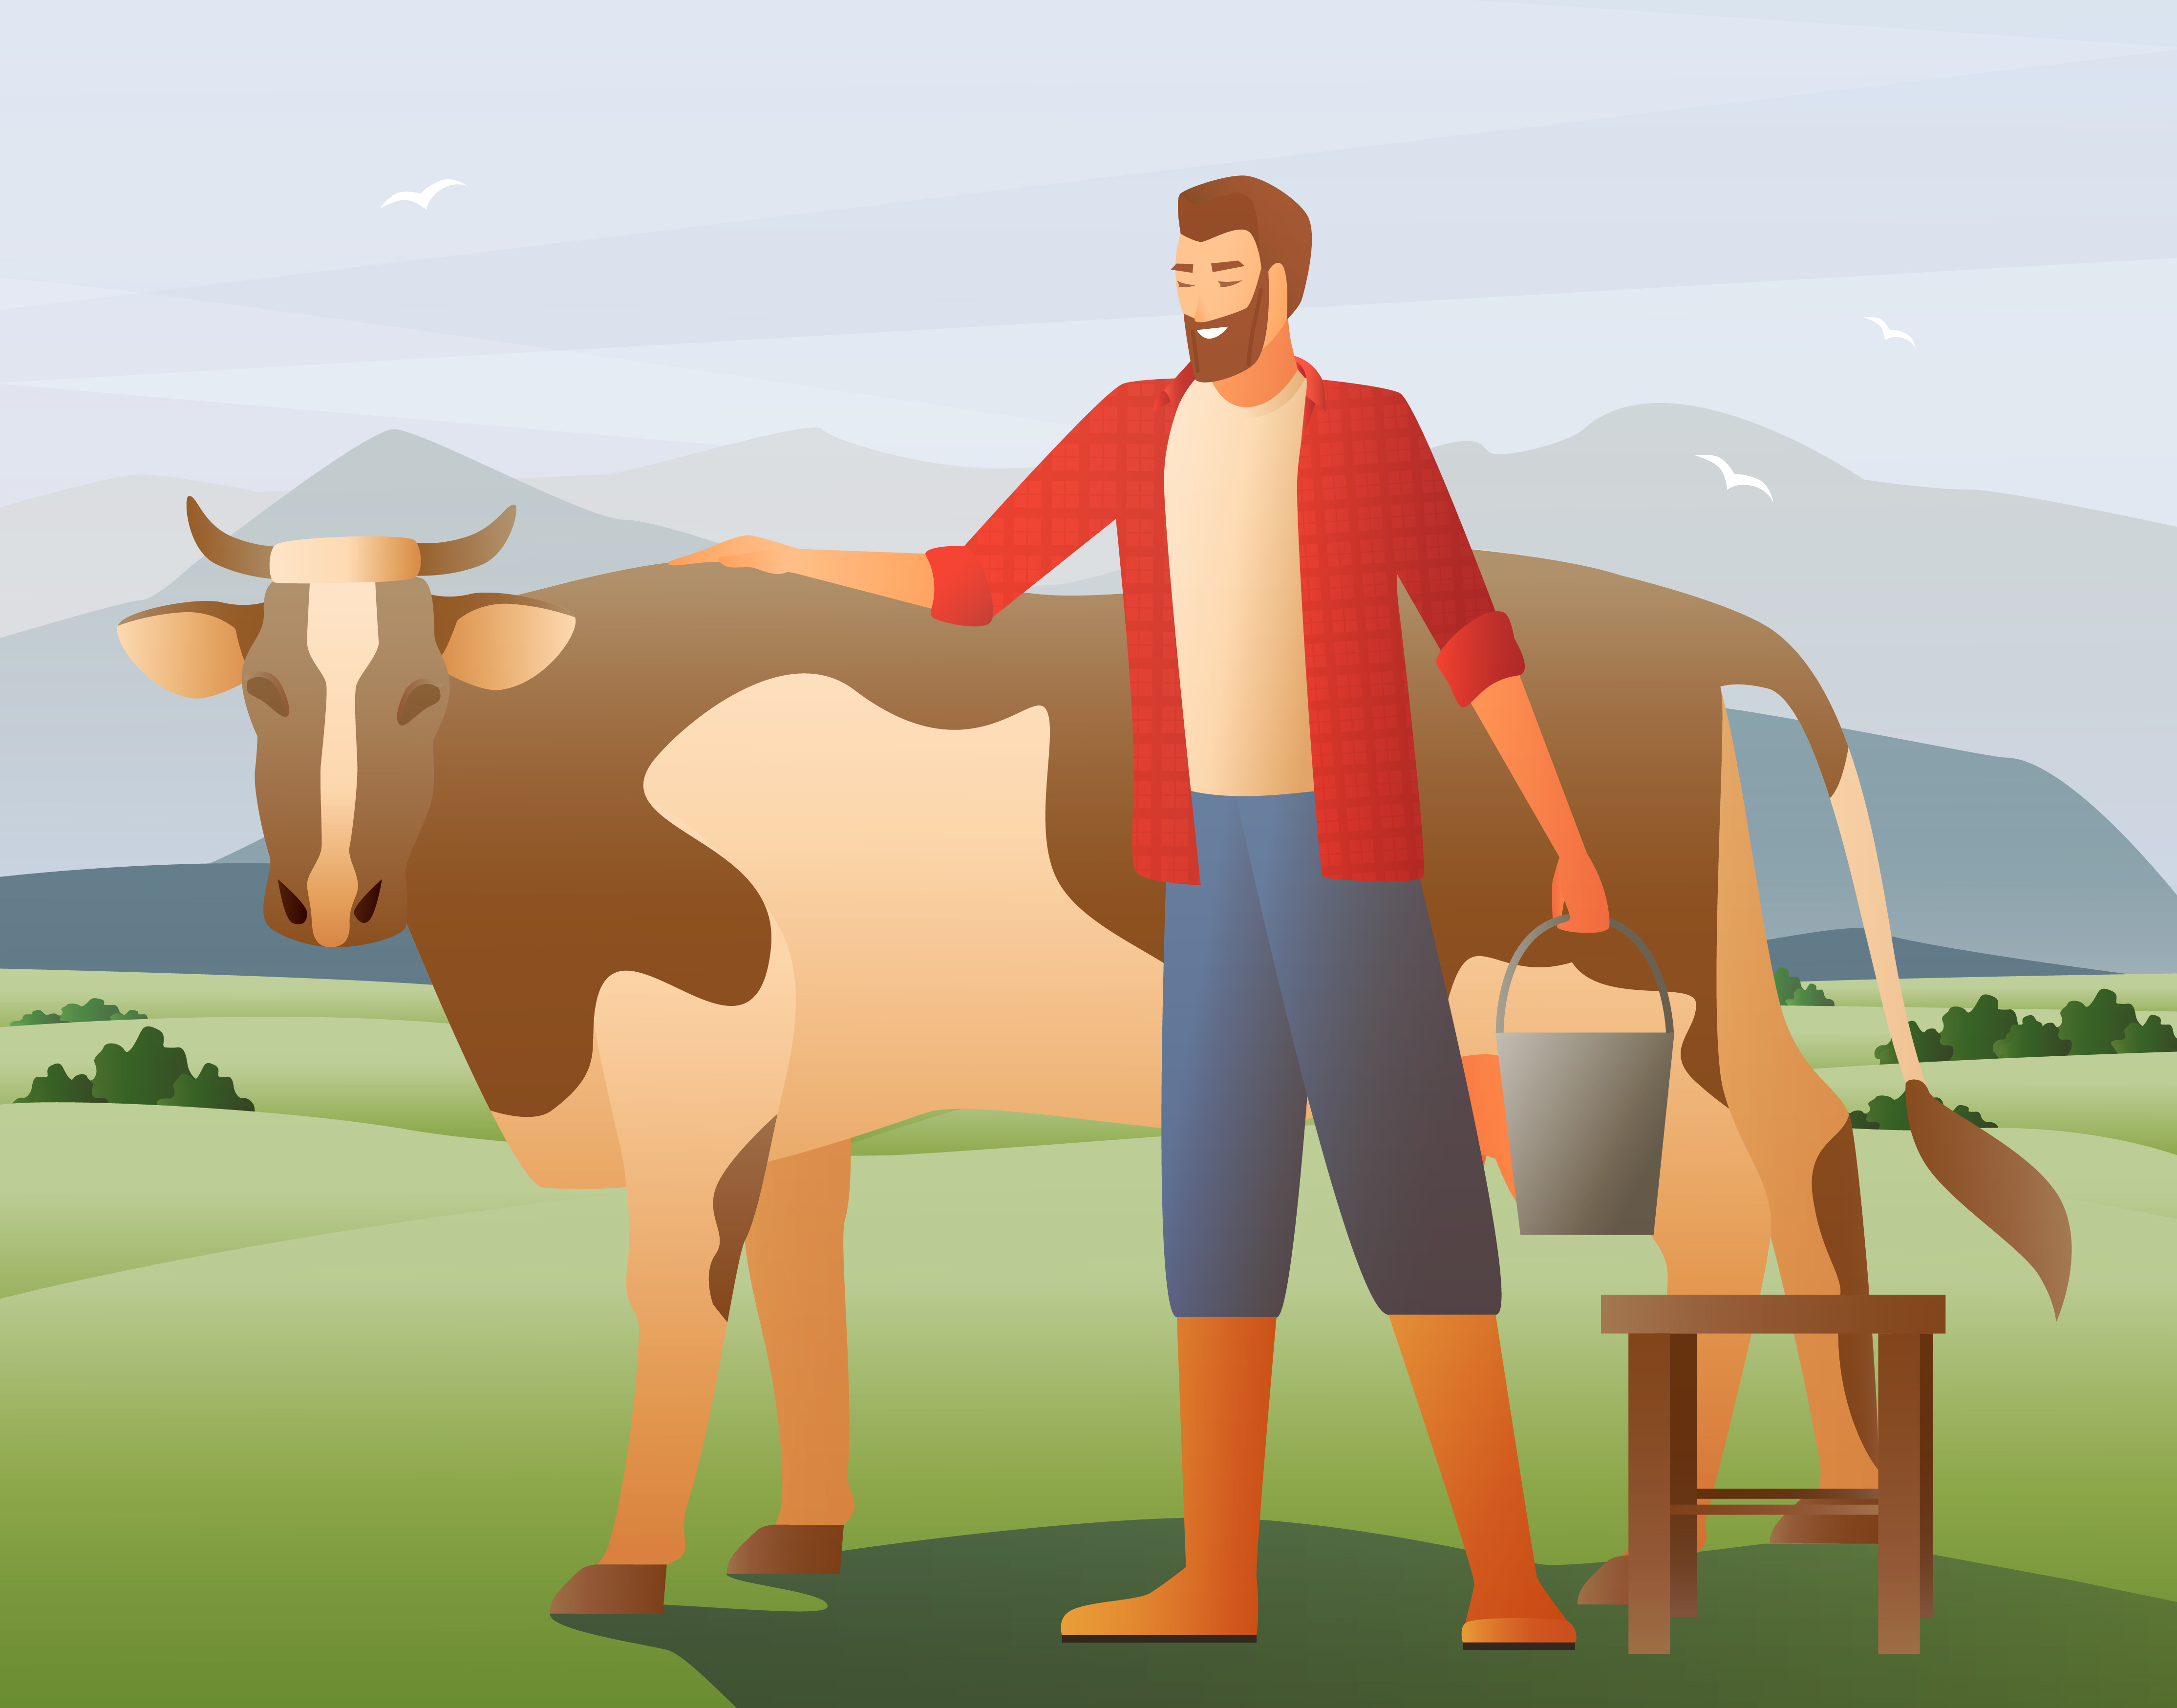
\includegraphics[width=1.16587in,height=0.93269in]{media/image50.jpeg}
\includegraphics[width=1.42308in,height=1.21950in]{media/image51.jpeg}
\end{figure}

\reduline{Apito\hfill}

\reduline{Bicicleta\hfill}

\reduline{Árvore\hfill}

\begin{figure}[htpb!]
\includegraphics[width=1.10833in,height=1.00903in]{media/image52.jpeg}
\includegraphics[width=0.85556in,height=0.92222in]{media/image53.jpeg}
\includegraphics[width=0.79808in,height=0.79808in]{media/image54.jpeg}
\end{figure}

\reduline{Bola\hfill}

\reduline{Raposa\hfill}

\reduline{Gaiola\hfill}

\begin{figure}[htpb!]
\includegraphics[width=0.91319in,height=1.16319in]{media/image55.jpeg}
\includegraphics[width=1.62569in,height=1.25000in]{media/image56.jpeg}
\includegraphics[width=0.93990in,height=1.27885in]{media/image57.jpeg}
\end{figure}

\reduline{Pera\hfill}

\reduline{Pedra\hfill}

\reduline{Unha\hfill}

\pagebreak
\num{2} Separe as sílabas das palavras, depois circule as sílabas formadas por
consoante + consoante + vogal.

%\coment{Leia as palavras com os alunos, orientando-os a identificar vogais e consoantes. Também é possível montar algumas palavras com o alfabeto móvel. Em seguida, peça a eles que batam palmas cada vez que um pedacinho da palavra for pronunciado.}

\begin{longtable}[]{@{}ll@{}}
\toprule
\textbf{PRATO} & \rosa{Pra - to}\tabularnewline
\midrule
\textbf{FORMIGA} & \rosa{For- mi -ga}\tabularnewline
\midrule
\textbf{BRAÇO} & \rosa{Bra -ço}\tabularnewline
\midrule
\textbf{DRAGÃO} & \rosa{Dra- gão}\tabularnewline
\midrule
\textbf{CRAVO} & \rosa{Cra -- vo}\tabularnewline
\bottomrule
\end{longtable}

\num{3} Ligue as palavras com seu desenho.

%\coment{Leve para sala as palavras dentro de uma sacola. Cada criança deve pegar uma palavra da sacola para fazer a leitura. Depois proponha a atividade.}

Bicicleta \hfill\includegraphics[width=.1\textwidth]{media/image59.png}

Janela \hfill\includegraphics[width=.1\textwidth]{media/image60.png}

Borboleta \hfill\includegraphics[width=.1\textwidth]{media/image61.png}

Dragão \hfill\includegraphics[width=.1\textwidth]{media/image62.png}

Avião \hfill\includegraphics[width=.1\textwidth]{media/image63.png}

Prego \hfill\includegraphics[width=.1\textwidth]{media/image64.jpeg}

Pomba \hfill\includegraphics[width=.1\textwidth]{media/image65.png}

Manga \hfill\includegraphics[width=.1\textwidth]{media/image66.png}


\pagebreak
\num{4} Pinte no diagrama as palavras do quadro abaixo.

%\coment{Faça a leitura das palavras com os alunos aproveite esse momento para trabalhar a função da escrita.}

\begin{quote}\parindent=0em
\vspace*{-.5cm}
\begin{multicols}{3}
PIÃO

CAMA

LEÃO

PEDRA

ABACATE

SAPO

PATO

SABÃO

TRATOR

GRAMA

CISNE
\end{multicols}
\end{quote}

\begin{longtable}[]{@{}llllllllll@{}}
\toprule
P & I & Ã & O & D & O & W & E & I & S\tabularnewline
F & H & P & I & S & A & B & Ã & O & A\tabularnewline
S & J & L & S & J & U & Y & U & J & P\tabularnewline
L & O & A & B & A & C & A & T & E & O\tabularnewline
E & U & I & D & A & S & A & L & K & A\tabularnewline
à & A & B & G & C & A & Y & J & G & P\tabularnewline
O & S & A & P & A & T & O & P & R & E\tabularnewline
Z & D & R & F & D & M & E & C & A & D\tabularnewline
L & T & R & A & T & O & R & Q & M & R\tabularnewline
B & U & G & T & E & Y & E & & A & A\tabularnewline
A & C & I & S & N & E & O & P & U & O\tabularnewline
L & O & L & O & C & A & M & A & A & G\tabularnewline
\bottomrule
\end{longtable}

%\coment{R: pião -- cama -- leão- pedra- abacate- sapo- cama- pato -- sabão -- trator -- grama- cisne.}

\num{5} Coloque o til nas palavras sempre que necessário.

%\coment{Construa com os alunos critérios para identificar as marcas de nasalidade de uma palavra. Sugira que leiam as palavras em voz alta e posicionem os dedos indicador e polegar sobre o nariz ao pronunciar palavras com esses sons, para perceberem a diferença, por exemplo, entre a pronúncia de palavras como \textit{lá} e \textit{lã}, \textit{manha} e \textit{manhã}. Explique que o til acompanha apenas as vogais A e O.}

\begin{multicols}{3}
IRMAO

SALA

MAO

PATO

MAÇA

VILA

MOLA

MANHA

LA
\end{multicols}

\num{6} Observe a marca de nasalização e complete as palavras com M ou N.

%\coment{Siga as orientações da questão anterior, aguçando a atenção das crianças quanto à diferença de pronúncia de palavras como \textit{pote} e \textit{ponte} e \textit{rapa} e \textit{rampa}. Reforce a ideia de M sempre antes de B, e N antes de outras consoantes.}

\begin{multicols}{3}
LÂ\reduline{M}PADA

CA\reduline{M}PO

LARA\reduline{N}JA

TRO\reduline{N}CO

VE\reduline{N}TO

PO\reduline{M}BA

U\reduline{M}BIGO

PO\reduline{N}TE

RA\reduline{M}PA

BO\reduline{M}BOM

TE\reduline{M}PO

PI\reduline{N}TA
\end{multicols}

\num{7} Observe as imagens e escreva uma frase para cada uma.

%\coment{Explore as imagens com as crianças e oriente a construção das frases.}

\begin{figure}[htpb!]
\centering
\includegraphics[width=.5\textwidth]{media/image67.jpeg}
\end{figure}

\reduline{Uma resposta possível é \textit{As crianças andam a cavalo}.\hfill}
\linhas{1}

\begin{figure}[htpb!]
\centering
\includegraphics[width=.5\textwidth]{media/image68.jpeg}
\end{figure}

\reduline{Uma resposta possível é \textit{A menina leva flores no carrinho}.\hfill}
\linhas{1}

\pagebreak
\num{8} Leia as frases a seguir e faça um desenho para representar.

%\coment{Oriente a leitura das frases explorando com as crianças o conteúdo de cada uma delas e as diferentes possibilidades de representação.}

\begin{myquote}
O CAVALO GOSTA DE CORRER.
\end{myquote}

\begin{mdframed}[linewidth=2pt,linecolor=salmao]
\vspace{7cm}
\end{mdframed}

\begin{myquote}
O MENINO JOGA BOLA.
\end{myquote}

\begin{mdframed}[linewidth=2pt,linecolor=salmao]
\vspace{7cm}
\end{mdframed}

\begin{myquote}
O PÁSSARO CANTA FELIZ.
\end{myquote}

\begin{mdframed}[linewidth=2pt,linecolor=salmao]
\vspace{7cm}
\end{mdframed}

\begin{myquote}
A ÁRVORE CAIU.
\end{myquote}

\begin{mdframed}[linewidth=2pt,linecolor=salmao]
\vspace{7cm}
\end{mdframed}

%\coment{Respostas pessoais dos alunos.}

\num{9} Forme palavras de acordo com a numeração, depois forme uma frase.

%\coment{Oriente os alunos a formar as palavras. Em seguida, trabalhe a função social de cada palavra para facilitar a construção das frases.}

\begin{longtable}[]{@{}lllll@{}}
\toprule
\begin{minipage}[b]{0.19\columnwidth}\raggedright\strut
1

BO\strut
\end{minipage} & \begin{minipage}[b]{0.19\columnwidth}\raggedright\strut
2

PI\strut
\end{minipage} & \begin{minipage}[b]{0.19\columnwidth}\raggedright\strut
3

NE\strut
\end{minipage} & \begin{minipage}[b]{0.19\columnwidth}\raggedright\strut
4

CO\strut
\end{minipage} & \begin{minipage}[b]{0.19\columnwidth}\raggedright\strut
5

ÃO\strut
\end{minipage}\tabularnewline
\midrule
\endhead
\begin{minipage}[t]{0.19\columnwidth}\raggedright\strut
6

CAM\strut
\end{minipage} & \begin{minipage}[t]{0.19\columnwidth}\raggedright\strut
7

BRA\strut
\end{minipage} & \begin{minipage}[t]{0.19\columnwidth}\raggedright\strut
8

CIS\strut
\end{minipage} & \begin{minipage}[t]{0.19\columnwidth}\raggedright\strut
9

CA\strut
\end{minipage} & \begin{minipage}[t]{0.19\columnwidth}\raggedright\strut
10

ÇO\strut
\end{minipage}\tabularnewline
\midrule
\begin{minipage}[t]{0.19\columnwidth}\raggedright\strut
11

MA\strut
\end{minipage} & \begin{minipage}[t]{0.19\columnwidth}\raggedright\strut
12

JA\strut
\end{minipage} & \begin{minipage}[t]{0.19\columnwidth}\raggedright\strut
13

LA\strut
\end{minipage} & \begin{minipage}[t]{0.19\columnwidth}\raggedright\strut
14

CA\strut
\end{minipage} & \begin{minipage}[t]{0.19\columnwidth}\raggedright\strut
15

PO\strut
\end{minipage}\tabularnewline
\bottomrule
\end{longtable}

\textbf{PALAVRA FRASE}

\begin{itemize}
\item 1 + 3 + 14 \reduline{\mbox{ }\hfill}

\item 7 + 10 \reduline{\mbox{ }\hfill}

\item 2 + 5 \reduline{\mbox{ }\hfill}

\item 6 + 15 \reduline{\mbox{ }\hfill}

\item 8 + 3 \reduline{\mbox{ }\hfill}

\item 12 + 3 + 13 \reduline{\mbox{ }\hfill}

\item 11 + 9 + 4 \reduline{\mbox{ }\hfill}
\end{itemize}

\num{10} Complete os nomes das frutas com as vogais corretas.

%\coment{Reapresente as vogais aos alunos de acordo com as palavras do exercício. Forme as palavras ressaltado sempre que não existe sílaba sem vogal.}

\begin{figure}[htpb!]
\includegraphics[width=.24\textwidth]{media/image69.jpeg}
\includegraphics[width=.24\textwidth]{media/image70.jpeg}
\includegraphics[width=.24\textwidth]{media/image71.jpeg}
\includegraphics[width=.24\textwidth]{media/image72.jpeg}
\end{figure}

\reduline{U}V\reduline{A} \hspace{1.5cm} L\reduline{A}R\reduline{A}NJ\reduline{A} \hspace{1cm} \reduline{A}B\reduline{A}C\reduline{A}X\reduline{I} \hspace{1cm} B\reduline{A}N\reduline{A}N\reduline{A}

\begin{figure}[htpb!]
\includegraphics[width=.24\textwidth]{media/image73.jpeg}
\includegraphics[width=.24\textwidth]{media/image74.jpeg}
\includegraphics[width=.24\textwidth]{media/image75.jpeg}
\includegraphics[width=.24\textwidth]{media/image76.jpeg}
\end{figure}

P\reduline{Ê}R\reduline{A} \hspace{1cm} M\reduline{O}R\reduline{A}NG\reduline{O} \hspace{1cm} G\reduline{O}\reduline{I}\reduline{A}B\reduline{A} \hspace{1cm} M\reduline{A}Ç\reduline{Ã}

\num{11} Organize as palavras de acordo com sua formação silábica.

%\coment{Leve o alfabeto para sala. Explore as vogais e as consoantes com os alunos. Realize com eles a formação de algumas palavras, identificado as diferentes formações silábicas. Brincar de \textbf{forca} é uma boa opção para desenvolver essa atividade.}

\begin{myquote}
ABACAXI -- TRATOR - GRAVIOLA - PRATO -- CAMPO - CISNE - BAÚ
\end{myquote}

{\small
\begin{tabular}{|l|l|l|l|}
\hline
\textbf{\begin{tabular}[c]{@{}l@{}}PALAVRAS COM\\ FORMAÇÃO CV\end{tabular}} & \textbf{\begin{tabular}[c]{@{}l@{}}PALAVRAS COM\\ FORMAÇÃO V\end{tabular}} & \textbf{\begin{tabular}[c]{@{}l@{}}PALAVRAS COM\\ FORMAÇÃO CCV\end{tabular}} & \textbf{\begin{tabular}[c]{@{}l@{}}PALAVRAS COM\\ FORMAÇÃO CVC\end{tabular}} \\ \hline
\rosa{ABACAXI} & \rosa{GRAVIOLA} & \rosa{TRATOR} & \rosa{CISNE} \\ \hline
\rosa{GRAVIOLA} & \rosa{ABACAXI} & \rosa{GRAVIOLA} & \rosa{CAMPO} \\ \hline
\rosa{PRATO} & \rosa{BAÚ} & \rosa{PRATO} &  \\ \hline
\rosa{CAMPO} &  &  &  \\ \hline
\rosa{CISNE} &  &  &  \\ \hline
\rosa{BAÚ} &  &  &  \\ \hline
\end{tabular}
}

\pagebreak
\colorsec{Treino}

\num{1} Mila foi à feira e comprou seu brinquedo preferido com as
econonias de seu cofrinho.

\begin{figure}[htpb!]
\centering
\includegraphics[width=.5\textwidth]{media/image77.jpeg}
\end{figure}

Qual palavra tem a primeira sílaba com a mesma formação da primeira
sílaba do nome do brinquedo de Mila?

\begin{multicols}{2}
\begin{escolha}
\item abacate.

\item janela.

\item traça.

\item prego.
\end{escolha}
\end{multicols}

\num{2} Leia a frase.

\begin{myquote}
\textbf{A menina brinca com bolhas de sabão.}
\end{myquote}

A imagem que representa o que está escrito na frase é

\begin{multicols}{2}
\begin{escolha}
\item\includegraphics[width=0.75159in,height=1.04531in]{media/image78.jpeg}

\item\includegraphics[width=1.23681in,height=1.10139in]{media/image79.jpeg}

\item\includegraphics[width=0.97361in,height=1.05069in]{media/image80.jpeg}

\item\includegraphics[width=0.75437in,height=1.04404in]{media/image81.jpeg}
\end{escolha}
\end{multicols}


\num{3} Veja a palavra nova que Ana aprendeu a ler.

\begin{myquote}
FORMIGA
\end{myquote}

A primeira sílaba da palavra acima tem a mesma formação que a 
primeira sílaba de

\begin{escolha}
\item borboleta.

\item dragão.

\item laranja.

\item garota.
\end{escolha}


\chapter[Encontrando informações no texto]{\Large Encontrando informações no texto}
\markboth{Módulo 3}{}

%Para iniciar este módulo, é possível comentar os tipos dos textos que serão lidos e explorar bastante a oralidade, fazendo diversos questionamentos de informações que estão nos textos.

\colorsec{Habilidade do SAEB}

\begin{itemize}
	\item Localizar informações explícitas em textos
\end{itemize}

\colorsec{Habilidades da BNCC}

\begin{itemize}
\item EF15LP03
\end{itemize}

\conteudo{

\begin{verse}
\textbf{Meu galinho}

Há três noites que eu não durmo\\
Ó lá lá\\
Pois perdi o meu galinho\\
O lá lá\\
Coitadinho o lá lá,\\
Pobrezinho o lá lá\\
Se perdeu lá no jardim.

Ele é branco e amarelo\\
O lá lá\\
Tem a crista vermelhinha\\
O lá lá\\
Bate as asas, o lá lá,\\
Abre o bico o lá lá\\
E faz qui qui ri qui qui
\end{verse}

\fonte{Disponível em: http://www.dominiopublico.gov.br/download/texto/me000588.pdf. Acesso em: 19 abr. 2023. }

Por que ele não dorme?

Onde o galo se perdeu?

Quais são as cores do galo?

Para responder a essas e outras perguntas, você precisa buscar as
informações no texto. Elas estão todas lá, de forma bem clara. 
Basta observar com atenção.

Observe o seguinte cartaz:\bigskip

\noindent\includegraphics[width=\textwidth]{media/image82.png}\bigskip

Está bem claro que esse cartaz contém um pedido de doação de brinquedos.
}

\colorsec{Atividades}

\num{1} Vamos cantar.

%\coment{Convide as crianças para brincar com a música, usando o nome dos alunos da turma. Em seguida faça questionamentos sobre a música: onde a canoa virou? Maria estava sozinha? Alguém socorreu Maria?}

\begin{quote}
\begin{verse}
\textbf{A canoa virou}

A canoa virou,\\
pois deixaram virar.\\
Foi por causa da maria,\\
que não soube remar.

Se eu fosse um peixinho\\
e soubesse nadar,\\
eu tirava a maria\\
do fundo do mar.
\end{verse}

\fonte{Política Nacional de Alfabetização. Cantigas. Disponível em: https://tinyurl.com/yckw7p6b. Acesso em: 19 abr. 2023. }
\end{quote}

\begin{escolha}
\item Escreva o título da música.

\reduline{A canoa virou.\hfill}
\linhas{1}

\item Por que a canoa virou?

\reduline{Maria não soube remar.\hfill}
\linhas{1}

\item Se eu fosse um peixinho o que eu faria?

\reduline{Se eu fosse um peixinho, eu tirava Maria do fundo do mar.\hfill}
\linhas{1}
\end{escolha}

\num{2} Vamos brincar de trem?

%\coment{Convide os alunos para formar um trem. Nesse momento, podem ser trabalhadas as noções de \textbf{lateralidade}: frente, trás, entre. Faça os questionamentos orais para trabalhar a fala e a escuta com as crianças.}

\begin{quote}
\begin{verse}
\textbf{O trem maluco}

O trem maluco,\\
quando sai de Pernambuco,\\
vai fazendo xique-xique\\
até chegar ao Ceará.
\end{verse}
\end{quote}

\begin{escolha}
\item  Encontre e circule o título da música.

\item De onde o trem sai?

\reduline{O trem sai de Pernambuco.\hfill}

\item Para onde o trem vai?

\reduline{O trem vai para o Ceará.\hfill}
\end{escolha}

\num{3} Vamos ler a letra da canção.\enlargethispage{2\baselineskip}

%\coment{Inicialmente, faça a leitura da letra da canção. Em seguida, convide as crianças a cantar. Depois, faça perguntas sobre o conteúdo da letra para trabalhar a oralidade.}

\begin{quote}
\begin{verse}
\textbf{Borboletinha}

Borboletinha\\
está na cozinha\\
fazendo chocolate\\
para a madrinha\\
poti,poti\\
perna de pau\\
olho de vidro\\
e nariz de pica-pau\\
tchau, tchau
\end{verse}

\fonte{Secretaria de Educação da Prefeitura de Diadema. Borboletinha. Disponível em: https://tinyurl.com/3n5ym7w5. Acesso em: 19 abr. 2023. }
\end{quote}

\begin{escolha}
\item Encontre e pinte de azul o nome da música.

\item Onde a borboletinha está?

\reduline{A borboletinha está na cozinha.\hfill}

\item O que ela está fazendo?

\reduline{A borboletinha está fazendo chocolate.\hfill}

\item Para quem é o cochocolate que ela está fazendo?

\reduline{A borboletinha está fazendo chocolate para a madrinha.\hfill}
\end{escolha}

\num{4} Observe esse cartaz.

%\coment{Pergunte as crianças o que elas vem no cartaz. Questione se já participaram de alguma campanha ou se já doaram roupas para outras pessoas. Aproveite e fale da importância de ser solidário.}

\begin{figure}[htpb!]
\centering
\includegraphics[width=.5\textwidth]{media/image83.jpeg}
\end{figure}
%\textbf{\url{http://www.saosebastiao.sp.gov.br/noticia.asp?id=N1122020143810.Acesso} 02 mar. 2023}

\begin{escolha}
\item Qual é a campanha mostrada no cartaz?

\reduline{O cartaz apresenta uma campanha de arrecadação de roupas.\hfill}

\item As roupas devem ser doadas a crianças de que idade?

\reduline{As roupas devem ser doadas a crianças de zero a 3 anos.\hfill}
\end{escolha}

\num{5} Vamos ler com atenção.

%\coment{Leia a receita para as crianças. Depois, pergunte a elas se conhecem esse tipo de texto. Identifique com elas as instruções apresentadas. A seguir, explore o conteúdo da receita, perguntando aos alunos, por exemplo, se conhecem os ingredientes e gostam deles.}

%Paulo: acredito que seria interessante colocar a receita abaixo em um box que lembrasse uma folha de papel, pautada ou não, se possível com uma fonte que lembre letra cursiva. 
\begin{quote}
\textbf{Macarrão de panela de pressão}

\textbf{Ingredientes}

%\includegraphics[width=1.94097in,height=1.14722in]{media/image84.jpeg}1

\begin{itemize}
\item 1 pacote de macarrão tipo parafuso

\item 1 saquinho molho de tomate

\item 1 caixa de creme de leite

\item Sal a gosto

\item Alho e cebola a gosto

\item 2 medidas do recipiente do molho de tomate de água

\end{itemize}

\textbf{Modo de fazer}

Em uma panela de pressão, frite o alho e a cebola. Depois, jogue o
macarrão e o molho de tomate e misture tudo. Aproveite o recipiente
do molho de tomate (o saquinho ou o pote): encha-o com água duas vezes
e jogue-a na panela.

Depois feche a panela e coloque no fogo. Assim que a panela pegar a
pressão, desligue, mas não abra e nem tire o pino: espere sair toda 
a pressão sozinha, lentamente. Quando isso acontecer, abra, mexa o
macarrão e coloque a caixa de creme de leite. Tempere com o sal a gosto.
Pronto! É só comer. 
\end{quote}

%Felipe ou Fábia: alterei esta receita (mandei mensagem no Odoo). Por isso, o link a seguir não é mais necessário: http://educacao.diadema.sp.gov.br/educacao/attachments/article/749/atividade\%209\%20semana\%20fase\%20I\%20Drummond.pdf.Acesso} 02 mar. 2023.
%https://www.freepik.com/premium-photo/spaghetti-dish-white-background\_4396472.htm\#query=MACARR\%C3\%83O\&position=8\&from\_view=search\&track=sph

\begin{escolha}
\item Qual é o nome do prato explicado na receita?

\reduline{O nome do prato explicado na receita é macarrão de panela de pressão.\hfill}

\item Encontre no texto e pinte de verde o nome do utensílio usado para
conzinhar o macarrão.

\reduline{O aluno deve pintar de verde a expressão ``panela de pressão''.\hfill}

\pagebreak
\item Agora escreva o nome de três ingredientes usados para fazer a receita.

\reduline{Os ingredientes usados para fazer a receita são macarrão, molho, creme de leite, sal, alho, cebola e água. O aluno deve escolher três deles.\hfill}
\end{escolha}

\num{6} Vamos cantar.

\begin{quote}
\begin{verse}
\textbf{Meu chapéu}

O meu chapéu tem três pontas,\\
tem três pontas o meu chapéu.\\
Se não tivesse três pontas,\\
não seria o meu chapéu.
\end{verse}

\fonte{Secretaria de Educação da Prefeitura de Diadema. Borboletinha. Disponível em: http://educacao.diadema.sp.gov.br/educacao/attachments/article/749/atividade\%209\%20semana\%20fase\%20I\%20Drummond.pdf. Acesso em: 19 abr. 2023. }
\end{quote}

\begin{escolha}
\item Quantas pontas tem o chapéu que aparece na canção?

\reduline{O chapéu descrito na letra da canção tem três pontas.\hfill}

\item Como você imagina que é esse chapéu? Desenhe.

\begin{mdframed}[linewidth=2pt,linecolor=salmao,roundcorner=10pt]
\coment{Resposta pessoal.}
\vspace{4cm}
\end{mdframed}
\end{escolha}

\num{7} Leia as informações do cartaz.

%\coment{Explore as informações do cartaz: a campanha de vacinação, o período em que acontece e a faixa etária a que se destina. Pergunte aos alunos se eles entendem o que significa a gotinha branca e peça-lhes que expliquem.}

\begin{figure}[htpb!]
\centering
\includegraphics[width=.5\textwidth]{media/image85.jpeg}
\end{figure}

%\url{https://barreiras.ba.gov.br/segunda-etapa-da-campanha-de-vacinacao-contra-o-sarampo-comeca-na-quinta-feira-14-em-barreiras/} Acesso 02 mar. 2023.

\begin{escolha}
\item Qual é a campanha divulgada no cartaz?

\reduline{A campanha divulgada no cartaz é a de vacinação contra o sarampo.\hfill}

\item Para quem é indicada essa vacinação?

\reduline{A vacinação é indicada para jovens e adultos de 20 a 29 anos.\hfill}

\item Em que período vai acontecer a campanha?
	
\reduline{A campanha vai acontecer de 18 a 30 de Novembro.\hfill}
\end{escolha}

\num{8} Leia o texto.

%\coment{Depois de cantar a canção e ler a letra, é interessante fazer uma dobradura do chapéu.}

\begin{quote}
\begin{verse}
\textbf{Marcha soldado}

Marcha soldado,\\
cabeça de papel.\\
Se não marchar direito,\\
vai preso pro quartel.

O quartel pegou fogo,\\
a polícia deu sinal.\\
Acode, acode, acode,\\
a bandeira nacional.
\end{verse}

\fonte{Política Nacional de Alfabetização. Cantigas. Disponível em: https://alfabetizacao.mec.gov.br/images/conta-pra-mim/livros/versao\_digital/cantigas\_versao\_digital.pdf. Acesso em: 19 abr. 2023. }
\end{quote}

\begin{escolha}
\item Localize no texto e pinte de vermelho como é a cabeça do soldado.

\item O que acontece com o soldado se não marchar direto?

\reduline{Se não marchar direito, o soldado vai preso.\hfill}

\end{escolha}

\num{9} Vamos cantar.

\begin{quote}
\begin{verse}
\textbf{Dona aranha}

A Dona Aranha subiu pela parede\\
veio a chuva forte e a derrubou\\
já passou a chuva\\
o sol já vai surgindo\\
e a Dona Aranha continua a subir
\end{verse}

\fonte{https://www2.bauru.sp.gov.br/arquivos/arquivos\_site/sec\_educacao/atividades\_pedagogica\_distancia/1;Infantil/49;EMEI\%20Maria\%20Elizabet\%20Camilo\%20de\%20P\%C3\%A1dua/5;PROF.\%C2\%AA\%20REBECA/Atividades\%20de\%2012\%20a\%2016\%20de\%20abril\_Infantil\%20II\%20B\_Prof\%C2\%AA\%20Rebeca.pdf.
Acesso 11 mar. 2023.}
\end{quote}

\begin{escolha}
\item Escreva o nome do animal que aparece na música.

\reduline{Aranha\hfill}

\pagebreak
\item Quem derrubou a Dona Aranha?

\reduline{A Dona Aranha foi derrubada pela chuva forte.\hfill}

\end{escolha}

\num{10} Vamos cantar.

\begin{quote}
\begin{verse}
\textbf{Pai Francisco}

Pai Francisco entrou na roda\\
tocando seu violão\\
vem de lá Seu Delegado\\
e Pai Francisco foi pra prisão.
\end{verse}
\end{quote}

%Tentei de todas as formas acessar a página a seguir, mas não consegui de jeito nenhum. Deve ser conteúdo restrito {http://servicos.rolandia.pr.gov.br/educacao/wp-content/uploads/aulas_online/cmeis/JOSEMARIA\%20ESCRIV\%C3\%81/INFANTIL-1/2021/16\%C2\%BAROT-I1B.pdf}Acesso 11 mar. 2023.

\begin{escolha}
\item Qual é o nome da canção?

\reduline{O nome da canção é ``Pai Francisco''.\hfill}

\item Desenhe o instrumento musical que Pai Francisco estava tocando.

\begin{mdframed}[linewidth=2pt,linecolor=salmao,roundcorner=10pt]
\vspace{8cm}
\end{mdframed}
\end{escolha}

\colorsec{Treino}

\num{1}

\begin{quote}
\begin{verse}
\textbf{Pintinho}

Meu pintinho amarelinho\\
cata aqui na minha mão,\\ 
na minha mão.\\
Quando quer comer bichinho,\\ 
com seu pezinho\\ 
ele cisca o chão.

Ele bate as asas,\\
ele faz piu-piu,\\ 
mas tem muito medo do gavião.
\end{verse}

\fonte{Domínio Público. Pintinho. Disponível em:
http://www.dominiopublico.gov.br/download/texto/me000588.pdf.
Acesso em: 19 abr. 2023.}
\end{quote}

O que o pintinho faz quando quer comer bichinho?

\begin{escolha}
	\item Cisca o chão.

	\item Bate as asas.

	\item Cata na mão.

	\item Faz piu-piu.
\end{escolha}

\pagebreak
\num{2} Leia o texto a seguir.

\begin{quote}
\begin{verse}
\textbf{Pombinha branca}

Pombinha branca \\
O que está fazendo?\\
Lavando a roupa\\
Do casamento.

A roupa é suja\\
É cor-de-rosa\\
Pombinha branca\\
É preguiçosa.

\end{verse}

\fonte{Domínio Público. Pombinha branca. Disponível em: http://www.dominiopublico.gov.br/download/texto/me000588.pdf. Acesso em: 19 abr. 2023.  }
\end{quote}

A pombinha é considerada preguiçosa porque

\begin{escolha}
	\item vai casar.

	\item a roupa está suja.

	\item só tem roupas cor-de-rosa.

	\item porque está lavando roupa.
\end{escolha}

\pagebreak
\num{3} Leia o texto.

\begin{quote}
\begin{verse}
\textbf{O tubo de cola}

O tubo de cola saiu da gaveta\\
caiu no tapete da sala.\\
a bola pulou no tapete melado e ficou colada na cola.\\
aí, a bola falou:\\
--- sapato, me ajuda!\\
o sapato ajudou.\\
deu um peteleco na bola\\
a bola melada colou no sapato.
\end{verse}

%Aqui temos um problema: o texto usado não está em área aberta do site. Não me preocupei com a diagramação do texto acima e da questão em geral.  

\fonte{https://portal.educacao.go.gov.br/wp-content/uploads/2021/04/Atividade-7-2o-ano-LP-LOCALIZAR-INFORMACOES-EXPLICITAS-EM-TEXTOS-E-EM-IMAGENS-GENERO-CONTOS.pd}
\end{quote}

De onde saiu o tubo da cola?

\begin{escolha}
\item DA BOLA

\item DO TAPETE.

\item DO SAPATO.

\item DA GAVETA.
\end{escolha}

\chapter{Para que serve este texto?}
\markboth{Módulo 4}{}

%Para iniciar o módulo, apresente os textos aos alunos pergunte se eles conhecem algum deles. Em seguida, explique a função de cada texto e a quem ele se destina.

\colorsec{Habilidade do SAEB}

\begin{itemize}
\item Reconhecer a finalidade de um texto.
\end{itemize}

\colorsec{Habilidade da BNCC}

\begin{itemize}
\item EF15LP01.
\end{itemize}

\conteudo{Você sabe para que servem os textos?

Existem vários tipos de textos, com linguagem e estrutura próprias e com 
diferentes funções.

Veja alguns deles e suas funções.

\includegraphics[width=.5\textwidth]{media/image86.jpeg}
\includegraphics[width=.5\textwidth]{media/image87.png}

\includegraphics[width=.5\textwidth]{media/image90.jpeg}
\includegraphics[width=.5\textwidth]{media/image92.png}
%\includegraphics[width=1.97452in,height=2.09063in]{media/image91.png}
}

%\textbf{https://www.flickr.com/photos/cbnsp/8264557482/in/photostream/}
%\textbf{https://agenciadenoticias.uniceub.br/sem-categoria/df-supera-80-mil-casos-suspeitos-de-dengue-e-ja-e-mais-que-o-triplo-do-total-do-ano-de-2021/}
%\textbf{https://www.freepik.com/free-photo/calendar-agenda-event-meeting-reminder-schedule-graphic-concept\_17132741.htm\#query=AGENDA\&position=30\&from\_view=search\&track=sph}

\colorsec{Atividades}

\num{1} Bel vai à padaria e quer deixar um aviso para sua tia. 
Marque com um X o texto que ela deve usar.

%\coment{Pergunte aos alunos se eles conhecem esses textos e explique a função de cada um deles.}

\includegraphics[width=.3\textwidth]{media/image93.jpeg}
\includegraphics[width=.3\textwidth]{media/image94.jpeg}
\includegraphics[width=.3\textwidth]{media/image97.png}

%\textbf{https://www.guarapari.es.gov.br/noticia/ler/285/setac-realiza-campanha-de-arrecadacao-de-roupas}

%\textbf{ttps://pt.wikipedia.org/wiki/Agenda\#/media/Ficheiro:Agenda.jpg}

\pagebreak

\num{2} Tamires vai convidar sua prima para a sua festa de formatura. 
Enconte e circule com lápis verde o texto que ela vai usar. 

%\coment{Retome as orientações anteriores para realizar a atividade.}

\includegraphics[width=.5\textwidth]{media/image100.png}
\includegraphics[width=.5\textwidth]{media/image103.png}

%\textbf{https://saltinho.sp.gov.br/paginas/portal/noticia?id=591}

\num{3} Pinte o quadrinho do texto que serve para informar o leitor.

%\coment{Explique a função de cada texto para a turma. Além disso, leve os nomes dos textos em uma caixinha e peça às crianças que sorteiem um deles. Depois, promova uma discussão sobre o texto sorteado.}

\begin{boxlist}
\boxitem{\white{X}} Convite

\boxitem{\white{X}} Notícia

\boxitem{\white{X}} Agenda 

\boxitem{\white{X}} Receita

\boxitem{\white{X}} Cartaz 

\boxitem{\white{X}} Tirinha
\end{boxlist}

\pagebreak
\num{4} No caça-palavras, existem sete nomes de tipos de textos. 
Encontre e pinte cada um deles.  

\begin{myquote}
\begin{multicols}{2}
AGENDA

NOTÍCIA

RECEITA

CONVITE

LISTA

VERBETE

TIRINHA
\end{multicols}
\end{myquote}

%\coment{Poderá usar a sugestão anterior para realizar a atividade.}

\begin{figure}[htpb!]
\includegraphics[width=\textwidth]{media/image104.jpeg}
\end{figure}

%\coment{Resposta: \includegraphics[width=2.42537in,height=2.09849in]{media/image105.jpeg}}

\pagebreak
\num{5} Observe esse texto.

%\coment{Leia o texto junto com as crianças. Em seguida, pergunte a elas se conhecem os ingredientes e se sabem como a receita deve ser seguida. Explique a função das receitas e onde geralmente elas são encontradas.}

\begin{figure}[htpb!]
\includegraphics[width=\textwidth]{media/image106.jpeg}
\end{figure}

%\textbf{https://www.flickr.com/photos/cbnsp/8263487889/in/photostream/ Acesso 03 mar. 2023.}

\begin{escolha}
\item Qual é o nome desse texto?

\reduline{O nome desse texto é ``receita''.\hfill}

\item Para que serve esse texto?

\reduline{A receita serve para ensinar a fazer comida.\hfill}

\item Escreva dois nomes de ingredientes da receita.

\reduline{Os ingredientes são iogurte, hortelã picada, suco de limão, azeite sal.\hfill}
\end{escolha}

\pagebreak
\num{6} Veja esse texto.

%\coment{Explore as informações do cartaz, fazendo, por exemplo, as seguintes perguntas: para que ele serve? A qual grupo é destinado? Quem o produziu?}

\begin{figure}[htpb!]
\includegraphics[width=\textwidth]{media/image107.jpeg}
\end{figure}

%\fonte{https://www.valparaiso.sp.gov.br/portal/noticias/0/3/794/valparaiso-realiza-campanha-de-vacinacao-contra-paralisia-infantil-e-sarampo. Acesso 03 mar. 2023.}

\begin{escolha}
\item Como é chamado esse texto?

\reduline{Esse texto é chamado de cartaz.\hfill}

\item Para que ele serve?

\reduline{Esse texto serve para informar sobre a vacinas.\hfill}

\item Para qual grupo ele é destinando?

\reduline{Esse texto é destinado às crianças.\hfill}
\end{escolha}

\pagebreak
\num{7} Tati gosta de contar história para divertir seus amigos.
Marque com um X o texto que ela deve usar.

\includegraphics[width=.5\textwidth]{media/image110.png}
\includegraphics[width=.5\textwidth]{media/image109.png}

\includegraphics[width=.5\textwidth]{media/image108.jpeg}

%\url{https://agenciadenoticias.uniceub.br/sem-categoria/df-supera-80-mil-casos-suspeitos-de-dengue-e-ja-e-mais-que-o-triplo-do-total-do-ano-de-2021/}
%https://lizeseusamigos.org.br/tirinhas/tirinhas-tres

\num{8} Produza um texto para organizar os itens de uma compra.

%\coment{Pergunte aos alunos se eles conhecem esse tipo de texto. Dialogue com eles sobre a função e estrutura de listas de compras.}

\begin{itemize}
\item \reduline{Resposta pessoal\hfill}

\item \reduline{\mbox{}\hfill}

\item \reduline{\mbox{}\hfill}

\item \reduline{\mbox{}\hfill}

\item \reduline{\mbox{}\hfill}

\item \reduline{\mbox{}\hfill}

\item \reduline{\mbox{}\hfill}
\end{itemize}

\pagebreak
\num{9} Fernanda tem uma reunião no dia 03 de março de 2023. Onde ela
deve anotar esse compromisso?

\reduline{Fernanda deve anotar o compromisso na agenda.\hfill}

\num{10} No dia do aniversário de Samanta, sua madrinha fez um bolo de
chocolate. Pinte o balão com o texto que ela usou para preparar o bolo.

\begin{figure}[htpb!]
\includegraphics[width=\textwidth]{media/confederado.png}
\end{figure}

\pagebreak
\colorsec{Treino}

\num{1} Observe o texto que ana recebeu de sua prima.

\begin{figure}[htpb!]
\includegraphics[width=.5\textwidth]{media/confederado2.png}
\end{figure}

%\textbf{\url{https://www.flickr.com/photos/cbnsp/8263487889/in/photostream/} Acesso 03 mar. 2023.}

Esse texto serve para

\begin{escolha}
	\item Ensinar.

	\item Informar.

	\item Convidar.

	\item Anunciar.
\end{escolha}

\pagebreak
\num{2} Observe o cartaz que Mariana colou no mural da farmácia.

\begin{figure}[htpb!]
\centering
\includegraphics[width=.6\textwidth]{media/image115.png}
\end{figure}

Esse cartaz é destinado aos donos de 

\begin{escolha}
	\item Gatos e cavalos.

	\item Cachorros e ovelhas.

	\item Cavalos e cachorros.

	\item Cachorros e gatos.
\end{escolha}

\num{3} João quer apresentar as características do seu animal selvagem
preferido para seus amigos.

O texto que ele vai usar é

\begin{escolha}
	\item Receita.

	\item Bilhete.

	\item Verbete.

	\item Notícia.
\end{escolha}

\chapter{Encontrando o assunto do texto}
\markboth{Módulo 5}{}

\vspace*{-1cm}
\enlargethispage{2\baselineskip}

\colorsec{Habilidade do SAEB}

\begin{itemize}
\item Inferir o assunto de um texto verbal.
\end{itemize}

%\coment{Para realizar as atividades desse módulo, é necessário ler junto com os alunos todos os textos, explorando a tipologia, título, personagens, e informações nele contidas, levantado hipóteses sobre do assunto dos diferentes textos.}

\conteudo{Para entender o assunto de um texto, você pode levantar
hipóteses, analisar, comparar, estabelecer relações a partir das
afirmações e das partes nele contidas.

Vamos ler o texto a seguir com atenção.

\begin{quote}
\textbf{A galinha e a pérola}

Uma galinha estava esfomeada, por isso começou a zanzar atrás do
galinheiro. Havia ali uma pequena lixeira dos humanos, que sempre
acabavam deixando cair algumas migalhinhas de pão ou pedacinhos de 
bolo saborosos, que a galinha petiscava com muito gosto. No meio
desses restos, a galinha mastigou uma pedra dura, mas muito preciosa:
``uma pérola!'', ela exclamou ``essa pedrinha 
brilhante vale muito para os humanos, mas não significa nada para
mim, que  preferia ter encontrado um grãozinho de milho para encher
a pança \ldots''. E continuou saboreando os restinhos. 

\textbf{Moral da história}: nem todo mundo dá valor para as mesmas
coisas. 
\end{quote}

O texto acima é chamado de \textbf{fábula}. Nele, um animal age
como ser humano. A \textbf{moral da história} orienta o leitor a
entender o assunto do texto. No caso da fábula acima, a pérola é
preciosa para os humanos, mas não tem importância para a galinha.
Podemos concluir, então, que o valor das coisas varia de acordo com
quem olha para elas. Esse é o assunto do texto.} 

\colorsec{Atividades}

\num{1} Leia o texto a seguir e depois responda às perguntas sobre ele. 

\begin{quote}
\textbf{O jovem gigante}

Era uma vez um filho de camponeses que não crescia mais do que sete
centímetros. Um dia, como era habitual, o pai o levou para passear no
campo. Uma forte ventania, entretanto, carregou o pequenino para bem
longe, até a porta de um castelo. Ali, um casal de gigantes passou a
cuidar do menino, que cresceu rapidamente e ficou enorme.

\fonte{Política Nacional de Alfabetização. O jovem gigante. Disponível em: Disponível
em:https://alfabetizacao.mec.gov.br/images/conta-pra-mim/livros/versao\_digital/o\_jovem\_gigante\_versao\_digital.pdf.
Acesso em: 20 abr. 2023.}
\end{quote}

\begin{escolha}
\item Encontre e escreva o título do texto.

\reduline{O título do texto é ``O jovem gigante.\hfill} 

\item Invente outro título para o texto.

\reduline{Resposta pessoal. O título deve corresponder ao conteúdo do texto.\hfill}

\item Qual é o assunto do texto?

\reduline{O assunto do texto é a vida de um menino que não crescia mais de sete centímetros, mas que acabou se tornando um gigante.\hfill}
\end{escolha}

\pagebreak
\num{2} Observe o cartaz:

%\coment{Explore os elementos do cartaz perguntando aos alunos o que enxergam na imagem e o que se comemora no dia 12 de outubro.}

\begin{figure}[htpb!]
\centering
\includegraphics[width=.8\textwidth]{media/image119.jpeg}
\end{figure}

%{\textbf{https://tonoticia.com.br/noticia/4336/prefeitura-de-gurupi-oferece-transporte-gratuito-para-criancas-curtirem-festa-nesta-quarta-feira}}

Responda:

\begin{escolha}
\item Qual é o assunto desse texto?

\reduline{O circo vai estar na cidade.\hfill}

\item Qual data importante será comemorada?

\reduline{Dia das crianças.\hfill}
\end{escolha}

\num{3} Leia:

%\coment{Leia o texto e, em seguida, faça perguntas às crianças a respeito da estória. Peça sugestões para o título.}

\begin{quote}
Certa manhã, um ratinho saiu do buraco pela primeira vez.

Queria conhecer o mundo e travar relações com tanta coisa bonita de que
falavam seus amigos. Admirou a luz do sol, o verdor das árvores, a
correnteza dos ribeirões, a habitação dos homens, e acabou penetrando no
quintal duma casa da roça.

--- Sim senhor! É interessante isto!

Examinou tudo minuciosamente, farejou a tulha de milho e a estrebaria.
Em seguida, notou no terreiro um certo animal de belo pelo que dormia
sossegado ao sol.

\fonte{https://5ca0e999-de9a-47e0-9b77-7e3eeab0592c.usrfiles.com/ugd/5ca0e9\_32e028a1edf14c648545dfb939a18363.pdf}
\end{quote}

Responda:

\begin{escolha}
\item Crie um título para o texto.

\reduline{Resposta pessoal.\hfill}

\item Qual era o animal que estava no terreiro? Pinte o balão com a resposta certa.

\item Qual é o assunto desse texto?

\reduline{A primeira vez que o ratinho saiu do buraco.\hfill}
\end{escolha}

\num{4} Vamos ler o texto:

%\coment{Faça a leitura com os alunos; em seguida, pergunte o que entenderam a respeito do texto e qual lição ele traz para nossas vidas.}

\begin{quote}
\textbf{O fazendeiro e a raposa}

Um fazendeiro ficou muito aborrecido com uma raposa que estava rondando o
seu quintal à noite e roubando as suas galinhas. Montou, então, uma
armadilha e a capturou. Para se vingar, amarrou um ramo de estopa
a sua cauda, colocou fogo e a soltou.

Para a sua má sorte, a raposa foi diretamente para os campos onde o milho
estava maduro e pronto para ser colhido. Ele pegou fogo e o fazendeiro perdeu toda a sua colheita.

\fonte{https://www.fabulasdeesopo.com.br/p/o-fazendeiro-e-raposa.html (Adaptado.)}
\end{quote}

Agora responda:

\begin{escolha}
\item Pinte o título do texto com a cor amarela.

\item Escreva o nome dos personagens do texto.

\reduline{A galinha, a raposa e o fazendeiro.\hfill}

\item Marque certo ou errado.

\begin{boxlist}
\boxitem{\white{X}} No texto, ao se vingar da raposa, o fazendeiro se deu bem.

\boxitem{\white{X}} No texto, ao se vingar da raposa, o fazendeiro também se prejudicou.

\boxitem{\white{X}} No texto, a armadilha do fazendeiro não funcionou.

\boxitem{\white{X}} No texto, o fazendeiro salvou sua colheta.
\end{boxlist}
\end{escolha}

\num{5} Leia o conto.

%\coment{Faça a leitura do texto com os alunos, perguntado a respeito do que entenderam sobre o texto.}

\begin{quote}
\textbf{Rumpelstichen}

Era uma vez um moleiro muito pobre, que tinha uma filha linda.

Um dia ele se encontrou com o rei e, para se dar importância,
disse que sua filha sabia fiar palha, transformando-a em ouro.

--- Esta é uma habilidade que me encanta --- disse o
rei. --- Se é verdade o que diz, traga sua filha amanhã cedo ao
castelo, eu quero pô-la à prova.

No dia seguinte, quando a moça chegou, o rei levou-a
para um quartinho cheio de palha, entregou-lhe uma roda e uma
bobina e disse:

--- Agora, ponha-se a trabalhar. Se até amanhã cedo
não tiver fiado toda esta palha em ouro, você morrerá! ---
depois saiu, trancou a porta e deixou a filha do moleiro
sozinha.

A pobre moça sentou-se num canto e, por muito tempo,
ficou pensando no que fazer. Não tinha a menor ideia de como
fiar palha em ouro e não via jeito de escapar da morte. O
pavor tomou conta da jovem, que começou a chorar
desesperadamente.

\fonte{Dísponível em: http://www.dominiopublico.gov.br/download/texto/me001614.pdf}
\end{quote}

\begin{escolha}
\item Escreva o nome da história.

\reduline{Rumpelstichen\hfill}

\item Quem são os personagens da história?

\reduline{O moleiro, sua filha e o rei.\hfill}

\item Qual é o assunto do texto?

\reduline{A mentira do moleiro.\hfill}
\end{escolha}

\num{6} Leia:

\begin{quote}
\begin{verse}
\textbf{A galinha do vizinho}

A galinha do vizinho\\
Bota ovo amarelinho\\
Bota um, bota dois,\\
Bota três, bota quatro,\\
Bota cinco, bota seis,\\
Bota sete, bota oito,\\
Bota nove, bota dez.
\end{verse}
\end{quote}

Responda:

\begin{escolha}
\item Qual é o assunto desse texto?

\reduline{A quantidade de ovos que a galinha do vizinho coloca.\hfill}

\item Pinte de azul o título do texto.
\end{escolha}

\num{7} Observe esse cartaz.

%\coment{Explore os elementos do cartaz e o que eles significam. Pergunte aos alunos se eles sabem o que as imagens com o traço vermelho significam.}

\begin{figure}[htpb!]
\centering
\includegraphics[width=.6\textwidth]{media/image120.jpeg}
\end{figure}

%\url{https://www.coronavirus.pr.gov.br/Imagem/Cartaz-Coronavirus} Acesso 04 mar. 2023.

Agora, responda:

\begin{escolha}
\item De qual doença trata o cartaz?

\reduline{A Covid-19\hfill}

\item Qual é a mensagem do cartaz?

\reduline{Como se prevenir para não pegar a doença.\hfill}
\end{escolha}

\num{8} Leia texto.

\textbf{A cegonha e a raposa}

\begin{figure}[htpb!]
\centering
\includegraphics[width=.2\textwidth]{media/image121.jpeg}
\includegraphics[width=.4\textwidth]{media/image122.jpeg}
\end{figure}

\begin{quote}
Um dia, a raposa, que era amiga da cegonha, convidou-a para jantar. Mas
preparou para a amiga uma porção de comidas moles, líquidas, que serviu
sobre uma pedra lisa.

Ora, a cegonha, com seu longo bico, por mais que se esforçasse só
conseguia bicar a comida, machucando o bico sem comer nada.

A raposa insistia para que a cegonha comesse, mas ela não conseguia, e
acabou indo para casa com fome. Em outra ocasião, a cegonha convidou a
raposa para jantar com ela.

\fonte{Disponível em: http://www.dominiopublico.gov.br/download/texto/me001614.pdf
Acesso em: 14 de fev. 2023.}
\end{quote}

Agora responda:

\begin{escolha}
\item Qual é o principal assunto do texto?

\reduline{O convite para jantar que a raposa fez para a cegonha.\hfill}

\item Quem participa da história?

\reduline{A raposa e a cegonha.\hfill}

\item Como você imagina o encontro mencionado no texto? %ilusatre.

\reduline{Resposta pessoal.\hfill}
\end{escolha}

\num{9} Observe o cartaz:

\begin{figure}[htpb!]
\centering
\includegraphics[width=\textwidth]{media/image123.jpeg}
\end{figure}

%https://urucui.pi.gov.br/dia-mundial-do-meio-ambiente-e-a-importancia-da-educacao-ambiental/

\begin{escolha}
\item Qual é o assunto do texto?

\reduline{Cuidados com o meio ambiente.\hfill}

\item Qual ação está sendo retratada no cartaz para a preservação do meio ambiente?

\reduline{A plantação de muda de árvores.\hfill}
\end{escolha}

\num{10} Vamos ler:

\begin{quote}
\textbf{O cão e o osso}

Um dia, um cão ia atravessando uma ponte carregando um osso na boca.
Olhando para baixo, viu sua própria imagem refletida
na água. Pensando ver outro cão, cobiçou-lhe logo o osso e
pôs-se a latir. Mal, porém, abriu a boca, seu próprio osso caiu
na água e se perdeu para sempre.

\fonte{Disponível em: http://www.dominiopublico.gov.br/download/texto/me001614.pdf}
\end{quote}

\begin{escolha}
\item De que fala o texto?

\reduline{A cobiça do cachorro pelo osso que enxergou em seu reflexo.\hfill}

\item O cachorro conseguiu pegar seu osso?

\reduline{Não, pois o osso caiu na água.\hfill}
\end{escolha}

\pagebreak
\colorsec{Treino}

\num{1}

\begin{figure}[htpb!]
\centering
\includegraphics[width=.6\textwidth]{media/image124.jpeg}
\end{figure}

%\textbf{Disponível em:https://tangaradaserra.mt.gov.br/site/?noticias=saude-divulga-nova-lista-de-convocacao-de-criancas-para-vacinacao-contra-covid-19Acesso em: 04 mar. 2023.}

O assunto do texto é

\begin{escolha}
\item Lista de vacinas.

\item Data da campanha.

\item Local de vacinação.

\item Vacinação para crianças.
\end{escolha}

\num{2} Leia a notícia:

\begin{quote}
\textbf{Nem eles se salvam: conheça os animais que sofrem com piolhos
como os humanos; veja alguns bem de pertinho}

\textit{As aves, além de mamíferos terrestres e aquáticos, também convivem com
ectoparasitas que podem causar doenças}

Os piolhos são parasitas externos que causam uma coceira tremenda na
pele, e não atingem só os humanos. Ocorrem também em mamíferos grandes
como os búfalos, pequenos como os gatos, aquáticos como a foca, e em
aves como as galinhas -- uma extensa lista de animais que podem se
tornar piolhentos.

\fonte{Disponível em:https://butantan.gov.br/bubutantan. Acesso em: 04 de Mar
2023.}
\end{quote}

O texto fala sobre

\begin{escolha}
\item O fato de os animais também sofrerem com piolhos.

\item Como os piolhos só afetam os humanos.

\item As características dos piolhos.

\item O fato de as aves serem os únicos animais que com piolhos.
\end{escolha}


\num{3} Leia o texto.

\begin{quote}
\textbf{A raposa inchada}

Uma raposa esfomeada encontrou, em uma árvore oca, uma quantidade de pão e
carne que alguns pastores tinham colocado lá para o seu regresso.
Encantada com o seu achado, ela entrou pela abertura estreita e devorou
tudo com avidez. Quando tentou sair, viu-se tão inchada depois da sua
refeição que não conseguia passar pelo buraco que entrou, choramingando e reclamando do seu infortúnio.

\fonte{https://www.fabulasdeesopo.com.br/p/a-raposa-inchada.html}
\end{quote}

De que fala essa fábula?

\begin{escolha}
\item Do alimento da raposa.

\item Do inchaço da raposa

\item Da gula da raposa.

\item Da fome da raposa.
\end{escolha}

\chapter[Encontrando as informações no texto]{\Large Encontrando as informações no texto}
\markboth{Módulo 6}{}

\colorsec{Habilidade do SAEB}

\begin{itemize}
\item
Inferir informações em textos verbais.
\end{itemize}

%\coment{Para realizar as atividades deste módulo, é necessário ler com os alunos todos os textos, explorando tipologias, títulos, personagens e informações neles contidas. Levante hipóteses sobre as informações que não foram apresentadas de forma explícita nos textos.}

\conteudo{

Vamos ler e pensar um pouco sobre o texto a seguir.

\begin{quote}
\begin{verse}
\textbf{Barata}

Eu vi uma barata\\
Na careca do vovô\\
Assim que ela me viu\\
Bateu asas e voou.
\end{verse}
\end{quote}

Você consegue imaginar porque a barata voou?

Veja que ela pode ter voado porque chegou alguém.

E por que o vovô tinha uma careca?

Porque seu cabelo caiu.

Observe que essas informaçãoes não estão ditas de forma clara no texto. Desse
modo, você precisa pensar um pouco para encontar respostas para as
perguntas.}

\pagebreak
\colorsec{Atividades}

\num{1} Leia o texto

\begin{quote}
\textbf{O gato de botas}

Um lavrador trabalhara muito, durante a vida toda, ganhando sempre o
suficiente para o sustento da família. Quando faleceu, deixou sua
herança para os filhos: um sítio, um burrinho e um gato.

Ao filho mais velho coube o sítio; ao segundo, o
burrinho; e o caçula ficou com o gato.
Este último, nada satisfeito com o que lhe coubera,
resmungou: "Meus irmãos sobreviverão honestamente. Mas, e eu?"

\fonte{Disponível em:
http://www.dominiopublico.gov.br/download/texto/me001614.pdf Acesso 04
mar. 2023.}
\end{quote}

Responda:

\begin{escolha}
\item O que o filho caçula ganhou de herança?

\reduline{Um gato.\hfill}

\item Como ele ficou quando recebeu a herança? Marque com o x.

\begin{boxlist}
\boxitem{\white{X}} Preocupado

\boxitem{\white{X}} Feliz

\boxitem{\white{X}} Animado

\boxitem{\white{X}} Triste
\end{boxlist}

\item O que explica sua reação?

\reduline{Ele ficou preocupado com sua sobrevivência, já que não sabia o que fazer para se sustentar apenas com o gato.\hfill}
\end{escolha}

\pagebreak
\num{2} Leia o texto

\begin{quote}
\begin{verse}
\textbf{Pombinha}

Pombinha quando tu fores\\
Me escreva pelo caminho\\
Se não achares papel\\
Nas asas de um passarinho.

Do bico faz um tinteiro\\
Da língua pena dourada\\
Dos dentes letra miúda\\
Dos olhos carta fechada.

A pombinha voou, voou\\
Foi-se embora e me deixou
\end{verse}

\fonte{Disponível
em: http://www.dominiopublico.gov.br/download/texto/me000588.pdf.
Acesso 04 mar. 2023.}
\end{quote}

\begin{escolha}
\item Por que a pombinha deverá escrever quando for embora?

\reduline{Para mandar notícias e amenizar a saudade que o eu lírico sente dela.\hfill}

\item Por que a pombinha deverá fazer do bico um tinteiro?

\reduline{Para escrever a carta.\hfill}

\end{escolha}

\pagebreak
\num{3} Vamos cantar.

%\coment{Cante com a turma e faça questionamentos sobre a letra da música.}

\begin{quote}
\begin{verse}
\textbf{Margarida}

Onde está a margarida?\\
Olê, olê, olá…

Onde está a Margarida?\\
Olê, seu cavaleiro.\\
Margarida está no castelo\\
Olê, olê, olá…\\
Margarida está no castelo\\
Olê, seu cavaleiro.

Eu queria ver a moça\\
Olê, olê, olá…\\
Eu queria ver a moça\\
Olê, seu cavaleiro.\\
Mas o muro é muito alto\\
Olê, olê, olá…
\end{verse}

\fonte{Disponível em: http://www.dominiopublico.gov.br/download/texto/me000588.pdf.
Acesso 04 mar. 2023}
\end{quote}

\begin{escolha}
\item Onde está Margarida? Circule no texto.

\item Por que não é possível ver a moça?

\reduline{Porque o muro do castelo é muito alto\hfill}

\item Pinte o quadrinho com a resposta correta:

Quem gostaria de ver Margarida?

\begin{multicols}{3}
\begin{boxlist}
\boxitem{\white{X}} O cavaleiro.

\boxitem{\white{X}} O rei.

\boxitem{\white{X}} Sua mãe.
\end{boxlist}
\end{multicols}

\end{escolha}

\pagebreak
\num{4} Leia a fábula a seguir.

%\coment{Fazer a leitura da fábula com os alunos, perguntando sobre os personagens e os ensinamentos que ela traz.}

\begin{quote}
\textbf{O leão e o ratinho}

Um leão, cansado de tanto caçar, dormia espichado à sombra de uma boa
árvore. Vieram uns ratinhos passear em cima dele e ele acordou. Todos
conseguiram fugir, menos um, que o leão prendeu embaixo da pata. Tanto o
ratinho pediu e implorou que o leão desistiu de esmagá-lo e deixou que
fosse embora.

Algum tempo depois, o leão ficou preso na rede de uns caçadores. Não
conseguia se soltar e fazia a floresta inteira tremer com seus urros de
raiva. Nisso, apareceu o ratinho. Com seus dentes afiados, roeu as
cordas e soltou o leão.

\fonte{https://conexaoeduca.saosebastiao.sp.gov.br/o-leao-e-o-ratinho-3o-ano/}
\end{quote}

Responda:

\begin{escolha}
\item Como você acha que o ratinho se sentiu quando o leão o pegou?

\reduline{Ele ficou com medo.\hfill}

\item Por que o leão deixou o ratinho ir embora?

\reduline{Porque teve compaixão.\hfill}

\item Por que o ratinho ajudou o leão?

\reduline{Porque um dia o leão tinha sido gentil com ele.\hfill}
\end{escolha}

\pagebreak
\num{5} Vamos ler o texto a seguir.

\begin{quote}
\begin{verse}
\textbf{Fui no mar}

Fui no mar buscar laranja\\
Coisa que o mar não tem\\
Voltei toda molhadinha\\
Das ondas que vão e vêm.
\end{verse}

\fonte{Disponível em: http://www.dominiopublico.gov.br/download/texto/me000588.pdf.Acesso 12 mar. 2023.}
\end{quote}

\begin{escolha}
\item Quem molhou a pessoa que foi ao mar?

\reduline{A água do mar.\hfill}

\item O que ela poderia ter encontrado no mar?

\reduline{Areia, água, conchinhas etc.\hfill}
\end{escolha}

\num{6} Leia:

%\coment{Ler o texto e comentar sobre essa fruta. Se possível, leve uma para apresentar aos alunos.}

\begin{quote}
\begin{verse}
\textbf{Caminho da roça}

No caminho da roça\\
Tem maracujá,\\
Mas não tem maduro\\
Pra meu bem chupar.

Dona mariquinha, olê {[}bis{]}\\
Dona mariquinha, olá
\end{verse}

\fonte{Disponível em: http://www.dominiopublico.gov.br/download/texto/me000588.pdf.
Acesso 12 mar. 2023.}
\end{quote}

Responda:

\begin{escolha}
\item Por que o maracujá não foi chupado?

\reduline{Porque ainda estava verde.\hfill}

\item Como é um maracujá verde? Desenhe.

\begin{mdframed}[linewidth=2pt,linecolor=salmao,roundcorner=10pt]
\coment{Resposta pessoal.}
\vspace{5cm}
\end{mdframed}
\end{escolha}

\num{7} Vamos cantar: função social da escrita

%\coment{Cantar a música com a turma e perguntar aos alunos se eles sabem onde são vendidos o violão e o pianinho. Explorar a função social da escrita das palavras.}

\begin{quote}
\begin{verse}
\textbf{Mestre André}

Foi na loja do mestre André\\
Que eu comprei um pianinho\\
Plim, plim, plim um pianinho\\
Ai ai olé ai ai olé\\
Foi na loja do mestre André.\\
Foi na loja do mestre André\\
Que eu comprei um violão\\
Dão dão dão um violão\\
Plim plim plim um pianinho
\end{verse}

\fonte{Disponível
em: http://www.dominiopublico.gov.br/download/texto/me000588.pdf.
Acesso em: 12 mar. 2023.}
\end{quote}

Responda:

\begin{escolha}
\item O que é vendido na loja do Mestre André?

\reduline{Instrumentos musicais.\hfill}

\item É possível comprar feijão na loja do Mestre André?

\reduline{Não\hfill}
\end{escolha}

\num{8} Vamos cantar.

\begin{quote}
\begin{verse}
\textbf{Fui morar numa casinha}

Fui morar numa casinha-nha\\
Infestada-da de cupim-pim-pim\\
Saiu de lá-lá-lá uma lagartixa-xa\\
Olhou pra mim, olhou pra mim e fez assim\\
Fui morar numa casinha-nha\\
Infestada-da de morceguinho-nho\\
Saiu de lá-lá-lá uma bruxinha-nha\\
Olhou pra mim, olhou pra mim e fez assim.
\end{verse}

\fonte{Disponivel em
:assimhttps://www2.bauru.sp.gov.br/arquivos/arquivos\_site/sec\_educacao/atividades\_pedagogica\_distancia/1;Infantil/46;EMEI\%20Maria\%20Alice\%20Seabra\%20Prudente/08;PROF.\%C2\%AA\%20FABIANA/Semana\%2008\%20-\%20\%20\%28De\%2019-04\%20a\%2023-04\%29\%20-\%20Infantil\%20II\%20-\%20Prof.\%20Rosana.pdf
Acesso em: 12 mar. 2023.}
\end{quote}

\begin{escolha}
\item Como era a casinha?

\reduline{Infestada de cupim e morceguinho.\hfill}

\item Por que a casa tinha cupim e morcego?

\reduline{Porque era uma casa antiga.\hfill}
\end{escolha}

\num{9} Vamos ler.

\begin{quote}
\begin{verse}
\textbf{Sai piaba}

Sai, sai, sai\\
Ó piaba,\\
Saia da lagoa.\\
Bota a mão na cabeça\\
Outra na cintura\\
Dá um remelexo no corpo\\
Dá uma umbigada\\
Na outra.
\end{verse}

\fonte{Disponível em
http://www.dominiopublico.gov.br/download/texto/me000588.pdf.
Acesso em: 12 mar. 2023.}
\end{quote}

Sabendo que a piaba é um tipo de peixe, ela poderia sair da lagoa? Por quê?

\reduline{Não, pois ela não vive fora da água.\hfill}

\num{10} Vamos cantar:

\begin{quote}
\begin{verse}
\textbf{Cai, cai balão}

Cai, cai balão\\
Cai, cai balão\\
Aqui na minha mão.\\
Não cai não, não cai não\\
Não cai não,\\
Cai na rua do sabão.
\end{verse}

\fonte{Disponível
em: http://www.dominiopublico.gov.br/download/texto/me000588.pdf Acesso
12 mar. 2023.}
\end{quote}

Onde o balão vai cair? Pinte no texto.

\colorsec{Treino}

\num{1}

\begin{quote}
\textbf{As árvores e o machado}

Havia uma vez um machado que não tinha cabo.
As árvores então resolveram que uma delas lhe daria
um cabo.

Um lenhador, encontrando o machado de cabo novo,
começou a derrubar a mata.

Uma árvore disse à outra:

--- Nós mesmas é que temos culpa do que está
acontecendo. Se não tivéssemos dado um cabo ao machado,
estaríamos agora livres dele.

\fonte{Disponível em
http://www.dominiopublico.gov.br/download/texto/me001614.pdf. Acesso
em 12 mar. 2023.}
\end{quote}

A árvore se sentiu culpada por ter dado o cabo ao machado porque ele

\begin{escolha}
\item Tinha um cabo novo.

\item Era feito de madeira.

\item Foi usado para cortar as árvores.

\item Foi encontrado pelo lenhador.
\end{escolha}

\num{2}

\begin{quote}
\textbf{O galo e a pérola}

Um galo estava ciscando, procurando o que comer no terreiro,
quando encontrou uma pérola. Ele então pensou:

--- Se fosse um joalheiro que te encontrasse, ia ficar feliz.
Mas para mim uma pérola de nada serve; seria muito melhor
encontrar algo de comer.

Deixou a pérola onde estava e se foi, para procurar
alguma coisa que lhe servisse de alimento.

\fonte{Disponível em
http://www.dominiopublico.gov.br/download/texto/me001614.pdf.
Acesso 12 mar. 2023.}
\end{quote}

O galo achou que um joalheiro ia gostar de encontrar a pérola porque ele

\begin{escolha}
\item Trabalha com joias.

\item Gosta de procurar tesouros.

\item Trabalha no terreiro.

\item Coleciona joias.
\end{escolha}


\num{3}

\begin{quote}
\begin{verse}
A linda rosa juvenil\\
A linda rosa juvenil,\\
Juvenil, juvenil\\
Vivia alegre no solar,\\
No solar, no solar\\
Vivia alegre no solar, no solar.

Mas uma feiticeira má,\\
Muito má, muito má\\
Mas uma feiticeira má,\\
Muito má\\
Adormeceu a rosa assim,\\
Bem assim, bem assim\\
Adormeceu a rosa assim,\\
Bem assim.

O tempo correu a passar,\\
A passar, a passar\\
O tempo correu a passar,\\
A passar.

O mato cresceu ao redor,\\
Ao redor, ao redor\\
O mato cresceu ao redor,\\
Ao redor.

Um dia veio um lindo rei,\\
Lindo rei, lindo rei\\
Um dia veio um lindo rei,\\
Lindo rei.

E despertou a rosa assim,\\
Bem assim, bem assim,\\
E despertou a rosa assim,\\
Bem assim.
\end{verse}

\fonte{Disponível em:
http://www.dominiopublico.gov.br/download/texto/me000588.pdf.
Acesso 12 mar. 2023.}
\end{quote}

A qual conto infantil a música se refere?

\begin{escolha}
\item Cinderela.

\item Branca de Neve.

\item A Bela Adormecida.

\item Chapeuzinho Vermelho.
\end{escolha}


\chapter{Os textos e as imagens}
\markboth{Módulo 7}{}

\colorsec{Habilidade do SAEB:}

\begin{itemize}
\item
Inferir informações em textos que articulam linguagem verbal e não verbal.
\end{itemize}

\colorsec{Habilidades da BNCC}

\begin{itemize}
\item EF15LP14.
\end{itemize}

%Explique o texto da introdução do módulo e leia a tirinha de forma clara, instigando as crianças a explicitarem o que entenderam.

\conteudo{Veja esse texto:

\noindent\includegraphics[width=.5\textwidth]{media/image125.jpeg}

%Disponível em: \url{https://iei-brasil.org/2021/12/21/mae-joana5/Acesso} 05 mar. 2023.

Você consegue perceber por que a mulher no primeiro quadrinho não queria ver a conta de luz?

Ela não quer ver porque imagina que a conta veio com um valor muito alto.

Você sabe dizer por que ela está com a mão na cabeça?

A mão na cabeça mostra que ela está preocupada.

Em alguns textos verbais e não verbais, as informaçãoes não são expostas de forma clara. Desse modo, você precisa pensar um pouco para encontrar respostas
para as perguntas. Elas aparecem, por exemplo, na expressão facial das personagens, mostrando as emocões que estão sentido, no formato dos balões de fala, nas onomatopeias, entres outros.}

\colorsec{Atividades}

\num{1} Observe o cartaz:

\begin{figure}[htpb!]
\centering
\includegraphics[width=.75\textwidth]{media/image128.png}
\end{figure}

%https://www.uberlandia.mg.gov.br/2022/01/27/mutirao-de-vacinacao-infantil-contra-a-covid-19/

\begin{escolha}
\item Qual público será vacinado nessa campanha?

\reduline{As crianças.\hfill}

\item Por que elas usam máscara?

\reduline{Para se proteger contra a doença.\hfill}
\end{escolha}

\pagebreak
\num{2} Leia o texto:

%\coment{Apresente vários tipos de balão e onomatopeias e explore seus significados.}

\begin{figure}[htpb!]
\includegraphics[width=.5\textwidth]{media/balao1.jpg}
\includegraphics[width=.5\textwidth]{media/balao2.jpg}
\end{figure}

\begin{escolha}
\item Quando o primeiro tipo de balão é usado?

\reduline{Esse balão é usado quando as personagens estão pensando.\hfill}

\item Quando o segundo tipo de balão é usado?

\reduline{Esse balão é usado quando as personagens estão gritando.\hfill}
\end{escolha}

\pagebreak
\num{3} Observe a imagem.

\begin{figure}[htpb!]
\includegraphics[width=\textwidth]{media/criancas.jpg}
\end{figure}

\begin{escolha}
\item O que as expressões faciais das garotas indicam?

\reduline{Sim, pois estão abraçadas.\hfill}

\item Você acha que as duas garotas são amigas? Por quê?

\reduline{Sim, pois estão abraçadas.\hfill}
\end{escolha}

\pagebreak
\num{4} Observe a imagem.

\begin{figure}[htpb!]
\includegraphics[width=\textwidth]{media/menina.png}
\end{figure}

\begin{escolha}
\item A expressão corporal da menina significa que ela está

\begin{boxlist}
\boxitem{\white{X}} Assustada.

\boxitem{\white{X}} Preocupada.

\boxitem{\white{X}} Animada.
\end{boxlist}

\item Por que a menina está assustada?

\reduline{Porque está com medo do fantasma.\hfill}

\end{escolha}

\pagebreak
\num{5} Veja esse cartaz:

\begin{figure}[htpb!]
\centering
\includegraphics[width=\textwidth]{media/image132.jpeg}
\end{figure}

%\url{https://www.aguasdelindoia.sp.gov.br/noticia/1416/fundo-social-de-aguas-de-lindoia-lanca-campanha-um-brinquedo-por-um-sorriso/}

\begin{escolha}
\item O que está sendo arrecadado nessa campanha?

\reduline{Brinquedos.\hfill}

\item Para quem os brinquedos serão entregues?

\reduline{Para as crianças.\hfill}
\end{escolha}

\pagebreak
\num{6} Veja a imagem:

\begin{figure}[htpb!]
\centering
\includegraphics[width=\textwidth]{media/image133.jpeg}
\end{figure}

%Disponível em: \url{https://igaratinga.mg.gov.br/conteudo/agua-economizar-e-melhor-do-que-ficar-sem\#.ZAXpcHbMIdU} .Acesso em: 06 mar. de 2023.

\begin{escolha}
\item O que a gota saindo da torneira representa?

\reduline{A água.\hfill}

\item Por que é importante economizar água?

\reduline{Para evitar a falta desse recurso.\hfill}
\end{escolha}

\pagebreak
\num{7} Observe o quadrinho:

\begin{figure}[htpb!]
\centering
\includegraphics[width=\textwidth]{media/image129.png}
\end{figure}

\begin{escolha}
\item Qual surpresa você acha que eles prepararam para Bele?

\reduline{Ela ia ganhar uma moto.\hfill}

\item O que mostra o tipo de balão usado no quadrinho?

\reduline{Que a mãe e o pai estão falando juntos.\hfill}
\end{escolha}

\pagebreak
\num{8} Observe o cartaz:

\begin{figure}[htpb!]
\centering
\includegraphics[width=\textwidth]{media/image134.jpeg}
\end{figure}

%Disponível em : \url{https://www.arceburgo.mg.gov.br/dengue-tambem-e-responsabilidade-de-todos/Acesso} 12 mar. 2023.

\begin{escolha}
\item Circule de azul o nome da doença que aparece no cartaz.

\item Circule de verde alguns cuidados que devemos tomar para combater essa doença.
\end{escolha}

\pagebreak
\num{9} Observe o cartaz:

\begin{figure}[htpb!]
\centering
\includegraphics[width=.8\textwidth]{media/image135.jpeg}
\end{figure}

%https://www.itupeva.sp.gov.br/noticias/para-celebrar-o-dia-das-criancas-a-festa-sera-no-parque-da-cidade

\begin{escolha}
\item A quem a festa é destinada?

\reduline{Às crianças.\hfill}

\item Em qual data ela será comemorada?

\reduline{No dia 12 de outubro, dia das crianças.\hfill}
\end{escolha}

\num{10} Agora é a sua vez. Escolha um tema e faça uma tirinha bem divertida.

\begin{mdframed}[linewidth=2pt,linecolor=salmao]
\vspace{4cm}
\end{mdframed}

\pagebreak
\colorsec{Treino}

\num{1} A expressão facial é um recurso usado nas histórias em quadrinhos.

\begin{figure}[htpb!]
\centering
\includegraphics[width=.35\textwidth]{media/alegre.png}
\end{figure}

Qual recurso foi usado para mostrar que a menina está feliz?

\begin{escolha}
\item O sorriso.

\item As mãos abertas.

\item As lágrimas.

\item A cor do cabelo.
\end{escolha}

\num{2} Veja a imagem:

\begin{figure}[htpb!]
\centering
\includegraphics[width=.4\textwidth]{media/image137.png}
\end{figure}

\pagebreak
%Disponível em: \url{https://www.amvapmg.org.br/1/campanha-de-vacinacao-contra-a-raiva-em-campina-verde-comecou-nesta-segunda-feira-17/ Acesso em: 12 mar. 2023.

Qual recurso visual foi usado para divulgar a campanha de vacinação?

\begin{escolha}
\item A mão segurando a vacina sobre o gato e o cachorro.

\item Os dois animais brincando.

\item Uma ilustração com diversos tipos de cachorros.

\item Crianças brincando com animais.
\end{escolha}

\num{3} Observe a imagem:

\begin{figure}[htpb!]
\centering
\includegraphics[width=.5\textwidth]{media/balao3.png}
\end{figure}

O formato do balão indica que

\begin{escolha}
\item Dormindo.

\item Gritando.

\item Pensando.

\item Cochichando.
\end{escolha}

% \colorsec{Referências bibliográfica}

% \begin{bibliohedra}
% \tit{MORAIS}.;A.G.; Ortografia: ensinar e aprender. São Paulo: Ática,1998

% \tit{CARVALHO}, Marlene. Alfabetizar e letrar: um diálogo entre a teoria e a
% pratica. 7. ed. Petrópolis, RJ: Vozes, 2010.

% \tit{FERREIRO}, Emília. Psicogênese da língua escrita. Porto Alegre: Artes
% médica sul, 1999.

% \tit{FERREIRO}, Emília. Psicogênese da língua escrita. Porto Alegre: Artes
% médica sul, 1999.

% \tit{INEP}. Instituto Nacional de Pesquisas Educacionais. \textbf{Sistema de
% Avaliação da Educação Básica:} Documento de Referência. Versão 1.0 1.
% ed. Brasília, DF: Ministério da Educação, v.1. 2018, 200 p.

% \tit{BRASIL}. Ministério da Educação. Conselho Nacional de Educação.~
% \textbf{Base Nacional Comum Curricular}. Brasília, DF: Ministério da
% Educação, 2018.
% \end{bibliohedra}



\pagebreak
\vspace*{-3.4cm}
%\hspace*{-3.7cm}\includegraphics[scale=1]{../watermarks/1simulado5ano.pdf}

%!TEX root=./LIVRO.tex
\setcounter{chapter}{0}
\chapter[Simulado 1]{Simulado}

\num{1} Observe o cartaz abaixo para responder à questão.


\includegraphics[width=5.90551in,height=2.125in]{./imgSAEB_7_POR/media/image16.png}

\fonte{Secretaria do Meio Ambiente do Estado do Amazonas. Campanha Floresta faz a diferença. 
Disponível em: https://meioambiente.am.gov.br/campanha-floresta-faz-a-diferenca/.
Acesso em: 22 mai. 23}

\noindent Acima, pode-se observar um cartaz de conscientização sobre o desmatamento da
Amazônia. O uso e repetição de determinadas palavras e imagens tem como
finalidade sensibilizar os leitores para o problema do desmatamento.
Sobre o uso da palavra ``floresta'', no cartaz, assinale a alternativa
correta.

\begin{escolha}

  \item Destacada à esquerda em letras grandes, uma parte da palavra ``floresta'' compõe um jogo com 
  palavras do texto no centro do cartaz.   

  \item A parte destacada da palavra ``floresta'', à esquerda, remete aos malefícios das queimadas e desmatamento que o cartaz pretende combater. 

  \item O destaque da palavra ``floresta'' não dialoga com ``diferença'' e ``diferente'', que se articulam para convidar a uma mudança de atitude.

  \item O uso da palavra ``floresta'', em destaque, à esquerda, dialoga com as imagens à direita sem remeter ao texto central do cartaz da campanha. 

\end{escolha}

\num{2} Leia o texto abaixo para responder à questão. 

\begin{myquote}
\textbf{Fumaça de queimadas chega a São Paulo}

\textit{Segundo especialistas, a grossa nuvem de fumaça começou com incêndios nos estados das regiões
Norte e Centro-Oeste.}

No dia 9 de sexta-feira, moradores da cidade de São Paulo relataram sentir
um forte cheiro de fumaça. Esse fenômeno estava relacionado com uma nuvem
de fumaça proveniente de queimadas que haviam ocorrido nos estados do
Amazonas, Acre e Mato Grosso. Especialistas já haviam alertado sobre a
propagação dessa nuvem sobre o Brasil, prevendo que atingiria também grande
parte do Centro-Oeste, do Paraná e até mesmo parte do estado de São Paulo.

Diante dessa situação, a Companhia Ambiental do Estado de São Paulo (CETESB)
iniciou uma investigação para analisar as condições do ar na região
metropolitana de São Paulo. A divisão de Qualidade do Ar da agência está
detalhando os dados provenientes das estações de monitoramento e se
comprometeu a fornecer informações mais consolidadas assim que concluírem sua
apuração.

\fonte{Fonte de pesquisa: Ingrid Oliveira e Carolina Figueiredo. Fumaça de queimadas do Amazonas chega a São Paulo; 
moradores relatam ``cheiro forte''. Disponível em:
https://www.cnnbrasil.com.br/nacional/fumaca-de-queimadas-do-amazonas-chega-a-sao-paulo-moradores-relatam-cheiro-forte/.
Acesso em: 22 mai. 2023.}

\end{myquote}

Assinale a alternativa que contém a parte da notícia denominada linha fina.

\begin{escolha}

\item ``moradores da cidade de São Paulo relataram sentir um forte cheiro de fumaça''.

\item ``Especialistas já haviam alertado sobre a propagação dessa nuvem sobre o Brasil''.

\item ``a Companhia Ambiental do Estado de São Paulo (CETESB)
iniciou uma investigação para analisar as condições do ar''.

\item ``Segundo especialistas, a grossa nuvem de fumaça começou com incêndios nos estados das regiões
Norte e Centro-Oeste''.

\end{escolha}

\num{3} Leia o texto abaixo para responder à questão.

\begin{myquote}
Uma parceria entre a Universidade Federal do Rio de Janeiro e a
Universidade Federal do Estado do Rio de Janeiro (Unirio) vem estudando
o vírus-T linfotrópico humano do tipo 1, o HTLV-1, retrovírus da mesma
família do HIV, associado a casos de leucemia e doenças
neurodegenerativas. A pesquisa recebeu investimento da Organização
Pan-Americana de Saúde (Opas/OMS) junto com outros estudos
latino-americanos e caribenhos que investigam doenças negligenciadas.
Embora descrito, na década de 1980, como um vírus associado ao câncer, o
HTLV ainda é pouco estudado e bastante desconhecido do público em geral.

\fonte{Carol Correia e Luana Reis.Conexão UFRJ. 
Pesquisa investiga vírus que pode levar à leucemia e neurodegeneração.
Disponível em: https://conexao.ufrj.br/2023/04/pesquisa-investiga-virus-negligenciado-que-pode-levar-a-doencas-neurodegenerativas-e-leucemia/.
Acesso em: 22 mai. 2023.}

\end{myquote}

O texto acima pertence ao gênero de divulgação científica, pois:

\begin{escolha}
  
  \item traz informações técnicas e de difícil compreensão.
  
  \item é escrito de maneira formal e dirigido a cientistas e estudiosos.
  
  \item traz informações sobre fatos do cotidiano.
  
  \item traz informações científicas em linguagem clara e acessível ao público.

\end{escolha}

\pagebreak

\num{4} Leia o texto abaixo para responder à questão.

\begin{myquote}

Ilma. Sra. Diretora da Escola Estadual Ulysses Guimarães:

Mariana Amaral Santos, aluna regularmente matriculada no sétimo ano do
Ensino Fundamental desta escola, vem respeitosamente solicitar à V.S.\textsuperscript{a} a
expedição dos documentos necessários à sua transferência para outro
estabelecimento de ensino.

Nestes termos, pede deferimento.

Curitiba, 24 de setembro de 2022.

\fonte{Texto adaptado para este material.}

\end{myquote}

O texto acima é um modelo de requerimento, pois tem como objetivo:

\begin{escolha} 

\item convencer o destinatário a realizar uma ação importante.

\item solicitar formalmente ao destinatário a realização de uma ação.

\item mudar o comportamento do destinatário a partir da realização de ações.

\item informar formalmente o destinatário acerca da solicitação de ações.

\end{escolha}

\num{5} Leia o texto abaixo para responder à questão.

\begin{myquote}

\textbf{ATO I}

\textbf{Cena I}

\textit{Veneza. Uma rua. Entram Antônio, Salarino e Salânio.}

ANTÔNIO -- Não sei, realmente, porque estou tão triste. Isso me enfara; e
a vós também, dissestes. Mas como começou essa tristeza, de que modo a
adquiri, como me veio, onde nasceu, de que matéria é feita, ainda estou
por saber. E de tal modo obtuso ela me deixa, que mui dificilmente me
conheço.

SALARINO -- Vosso espírito voga em pleno oceano, onde vossos galeões de
altivas velas -- como burgueses ricos e senhores das ondas, ou qual vista
aparatosa distendida no mar -- olham por cima da multidão de humildes
traficantes que os saúdam, modestos, inclinando-se, quando perpassam com
tecidas asas.

\fonte{William Shakespeare. O Mercador de Venza. 
Disponível em: http://www.dominiopublico.gov.br/download/texto/cv000094.pdf.
Acesso em: 22 mai. 2023.}

\end{myquote}

O trecho acima apresenta certas características, como discurso direto,
indicações de falas de personagens e rubricas, que são características 

\begin{escolha}

  \item das peças de teatro, textos escritos para encenação.

  \item dos poemas, compostos por versos e estrofes.

  \item dos contos, narrações curtas e de alto impacto.

  \item dos romances, narrativa longas e complexas.

\end{escolha}

\num{6} Leia o texto abaixo para responder à questão. 

\begin{myquote}

Os sites de fofoca são frequentemente alvo de críticas, mas eu sou
um firme defensor de sua existência. É um prazer de acompanhar a vida de celebridades
e figuras públicas, muitas vezes revelando verdades incômodas que a mídia tradicional 
ignora. Além disso, eles oferecem uma fonte interminável de diversão para milhões de
pessoas, servindo como uma fuga bem-vinda da monotonia da vida cotidiana. A
fofoca é sinal de uma cultura vibrante.

\fonte{Texto formulado para este material, escrito a partir de comentários 
em sites de fofoca e páginas de celebridades nas redes sociais.}

\end{myquote}

O texto acima contém muitas opiniões e poucos fatos. Há um fato
expresso no texto em:

\begin{escolha}

  \item ``Os sites de fofoca são frequentemente alvo de críticas''.
  
  \item ``É um prazer de acompanhar a vida de celebridades''.
  
  \item ``eles oferecem uma fonte interminável de diversão''.
  
  \item ``A fofoca é sinal de uma cultura vibrante''.

\end{escolha}

\num{7} Leia o texto abaixo para responder à questão.

%Alterei a questão. Rogério, 24/5/23, 10h13
%\includegraphics[width=4.16667in,height=1.57292in]{./imgSAEB_7_POR/media/image17.png}
%\fonte{http://www.arionaurocartuns.com.br/search?q=moradia}{\uline{http://www.arionaurocartuns.com.br/search?q=moradia}}.
%Acesso em 20 de Abr de 2023.

\begin{myquote}

É inútil descrever o quarto de um estudante: aí nada se
encontra de novo. Ao muito acharão uma estante, onde ele guarda
os seus livros, um cabide, onde pendura a casaca, o moringue, o
castiçal, a cama, uma até duas canastras de roupa, o chapéu, a
bengala e a bacia, a mesa, onde escreve e que só apresenta de
recomendável a gaveta cheia de papéis, de cartas de família, de
flores e fitinhas misteriosas: é pouco mais ou menos assim o
quarto de Augusto.

Agora ele está só. Às sete horas, desse quarto saíram três
amigos: Filipe, Leopoldo e Fabrício. Trataram da viagem no dia 
seguinte e retiraram-se descontentes.

\fonte{Joaquim Manuel de Macedo. \textit{A moreninha}.} 

\end{myquote}

% \fonte{Joaquim Manuel de Macedo. A moreninha. 
% Disponível em: http://objdigital.bn.br/Acervo_Digital/Livros_eletronicos/a_moreninha.pdf.
% Acesso em: 24 mai. 2023.}

Assinale a alternativa correta quanto aos trechos do texto.

\begin{escolha}
    
    \item ``\textbf{aí} nada se encontra de novo'': o termo destacado se refere a ``um estudante''.
    
    \item ``onde escreve'': o sentido da frase equivale a ``onde eles escrevem''.  
    
    \item ``o quarto de Augusto'': Augusto é o estudante cujo quarto é citado no início do parágrafo.  
    
    \item ``Agora \textbf{ele} está só'': o termo destacado refere-se a ``o quarto de Augusto''.   

\end{escolha}

\pagebreak

\num{8} Leia o texto abaixo para responder à questão. 

%Tirei a imangem abaixo e alterei a questão (Rogério, 24/5/23, 9h52)
%\includegraphics[width=5.90551in,height=1.72222in]{./imgSAEB_7_POR/media/image18.png}
%\fonte{https://tirasarmandinho.tumblr.com/search/amor}{\uline{https://tirasarmandinho.tumblr.com/search/amor}}.
%Acesso em 21 de Abr.

\begin{myquote}

--- Não diga isso, Camilo. Se você soubesse como eu tenho andado, por sua
causa. Você sabe; já lhe disse. Não ria de mim, não ria \ldots{}

Camilo pegou-lhe nas mãos, e olhou para ela sério e fixo. Jurou que lhe
queria muito, que os seus sustos pareciam de criança; em todo o caso,
quando tivesse algum receio, a melhor cartomante era ele mesmo. Depois,
repreendeu-a; disse-lhe que era imprudente andar por essas casas.

\end{myquote}

% \fonte{Machado de Assis. A cartomante. Disponível em: 
% http://www.dominiopublico.gov.br/download/texto/bv000257.pdf.
% Acesso em: 23 mai. 2023.}
\fonte{Machado de Assis. \textit{A cartomante}.}

O diálogo acima pertence ao conto ``A cartomante'', de Machado de Assis.
No primeiro parágrafo, Rita lamenta ao amante Camilo o que vem 
sofrendo por ele. Assinale a alternativa correta quanto aos 
referentes dos pronomes destacados.  

\begin{escolha}

  \item ``\textbf{Você} sabe; já \textbf{lhe} disse'': os pronomes se referem a Rita.
  
  \item ``Camilo pegou-\textbf{lhe} nas mãos'': o pronome se refere às mãos de Camilo.
  
  \item ``Jurou que \textbf{lhe} queria muito'': o pronome se refere a Camilo.
  
  \item ``disse-\textbf{lhe} que era imprudente'': o pronome se refere a Rita.

\end{escolha}

\num{9} Leia o texto abaixo para responder à questão.

\begin{myquote}

Para nós, indígenas, uma montanha não é apenas uma formação geológica, mas sim
uma pessoa sagrada. Ela é parte essencial da nossa vida e cultura, e a
respeitamos como tal. A montanha não é vista como um mero recurso econômico,
mas como um ser vivo que desempenha um papel vital em nossa história e
espiritualidade. 

\fonte{Texto fomulado para este material. Fonte de pesquisa: Ailton Krenak. \textit{Ideias para adiar o fim do mundo}. 2ª Ed. São Paulo:
Companhia da Letras, 2020.}

\end{myquote}

No texto acima, o autor

\begin{escolha}

  \item contou narrativas tradicionais da cultura indígena.

  \item comparou pontos de vista de indígenas e não indígenas.

  \item apresentou a língua falada pelo seu povo indígena.

  \item conciliou a cosmovisão de indígenas e não indígenas.

\end{escolha}

\num{10} Leia o texto abaixo para responder à questão.

\begin{myquote}

\textbf{Limpeza adequada evita crise alérgica e problemas
respiratórios}

Desde a infância, Maria Fulânima da Silva, aposentada de 53 anos, sofre com alergias, e
seus problemas respiratórios pioraram consideravelmente após o diagnóstico de
Lúpus, devido à sua baixa imunidade associada à doença. \textbf{Por causa disso}, ela
teve que intensificar os cuidados na organização de sua casa. Especialistas
advertem que pessoas alérgicas devem evitar acumular certos objetos,
especialmente no quarto, e, em vez de usar vassoura para a limpeza do chão,
recomendam o uso de um pano úmido. Eles também compartilham dicas sobre como
manter a residência limpa sem comprometer a saúde.

\fonte{Fonte de pesquisa: Jornal da Paraíba. Disponível em: https://jornaldaparaiba.com.br/bichos/faxina-correta-da-casa-evita-crise-alergica-e-possiveis-problemas-respiratorios/.
Acesso em: 2 out. 2023.}

\end{myquote}

No texto acima, a expressão destacada se refere:

\begin{escolha}
  
  \item à limpeza redobrada do ambiente.
  
  \item ao agravamento dos problemas respiratórios.
  
  \item à orientação médica sobre os cuidados com as crianças.
  
  \item à idade da paciente que precisa de cuidados.

\end{escolha}

\num{11} Leia o texto a seguir para responder à questão.

\begin{myquote}

O uso excessivo de celulares ocupa tempo precioso. As notificações constantes
e a busca por conteúdo online podem nos afastar do mundo real,
prejudicando nossa capacidade de conexão genuína com as pessoas ao nosso
redor. Além disso, o vício em smartphones é uma âncora que nos impede de
explorar as experiências e oportunidades que a vida tem a oferecer. Isso pode
levar a problemas de saúde mental, como ansiedade e depressão, bem como a uma
diminuição da produtividade e da qualidade de vida. É fundamental equilibrar
nosso uso de celulares para não nos perdermos no mundo virtual e manter um
vínculo sólido com a realidade que nos cerca.

\fonte{Texto formulado para este material.}

\end{myquote}

% \textbf{Sedentários e grudados a uma tela. O
% que mostra o maior estudo mundial sobre atividade física de
% jovens}

% Os especialistas já há algum tempo vêm alertando que os jovens não fazem todo o exercício físico que deveriam. Agora temos a confirmação: 80\% dos adolescentes (11 a 17 anos) em todo o mundo não fazem a atividade diária mínima para estarem saudáveis. E os especialistas não falam só de praticar esportes, e sim de ações básicas como caminhar até a escola ou jogar bola com os amigos no parque. Os padrões da Organização Mundial da Saúde (OMS) falam de uma hora diária de movimento. Estes dados ganham agora uma nova relevância se levarmos em conta a epidemia de obesidade que alcançou praticamente todos os países do mundo.

% \fonte{Patrícia Peiró. El País Brasil. Disponível em: https://brasil.elpais.com/brasil/2019/11/18/actualidad/1574086350_697117.html.
% Acesso em: 23 mai. 2023.}
%\fonte{Patrícia Peiró. El País Brasil.}

A frase que contém uso de figura de linguagem é:

\begin{escolha}
    
    \item ``O uso excessivo de celulares ocupa tempo precioso''.
    
    \item ``As notificações constantes e a busca por conteúdo online podem nos afastar do mundo real''.
    
    \item ``o vício em smartphones é uma âncora que nos impede de explorar as experiências''.
    
    \item ``pode levar a problemas de saúde mental, como ansiedade e depressão''.

\end{escolha}

\num{12} Leia o texto abaixo para responder á questão.

\begin{myquote}

Lisboa, situada em uma área geologicamente ativa, está sujeita à possibilidade
de ocorrer um grande terremoto nos próximos anos. A cidade já experimentou
eventos sísmicos significativos ao longo de sua história, como o terremoto de
1755, que causou devastação considerável. A região é parte da Zona de
Convergência da Eurásia e da África, onde as placas tectônicas se encontram,
aumentando o risco de atividade sísmica. Embora seja impossível prever com
precisão quando um novo evento pode ocorrer, as autoridades em Lisboa têm
tomado medidas de preparação e conscientização para minimizar os potenciais
danos e garantir a segurança da população.

\fonte{Texto formulado para este material.}

\end{myquote}

% \fonte{Oriol Güell. El País Brasil. Agência de saúde pública da UE avisa
% que a ômicron se propaga pelo continente mais rápido do que é detectada.
% Disponível em: https://brasil.elpais.com/internacional/2021-12-13/agencia-de-saude-publica-da-ue-avisa-que-a-omicron-se-propaga-pelo-continente-mais-rapido-do-que-e-detectada.html.
% Acesso em: 23 mai. 2023.}
%\fonte{Oriol Güell. El País Brasil.}

A expressão ``um novo evento'' se refere a:

\begin{escolha}
  
  \item ``um grande terremoto nos próximos anos''.
  
  \item ``o terremoto de 1755''.
  
  \item ``risco de atividade sísmica''.
  
  \item ``potenciais danos''.

\end{escolha}

\pagebreak

\num{13} Leia o texto abaixo para responder à questão. 

\begin{myquote}

A defesa da prática da leitura nas escolas brasileiras é respaldada por
estatísticas que evidenciam seus benefícios. De acordo com o último
levantamento do Instituto Pró-Livro, realizado em 2019, apenas 52\% da
população brasileira afirma ter lido ao menos um livro nos últimos três meses.
Esse número ressalta a necessidade de incentivar a leitura desde cedo, nas
escolas, como uma ferramenta poderosa para o desenvolvimento cognitivo e
educacional dos alunos. Além disso, dados do Programa Internacional de
Avaliação de Estudantes (PISA) demonstram que estudantes que têm o hábito de
leitura apresentam desempenho superior em todas as disciplinas, incluindo
matemática e ciências. Promover a leitura nas escolas não apenas
contribui para o crescimento intelectual dos estudantes, mas também pode ser
um meio eficaz de melhorar a qualidade da educação no Brasil.

\end{myquote}

% \fonte{Ana Cássia Maturano. G1. Opinião: como fazer de seu filho um leitor. 
% Disponível em: https://g1.globo.com/Noticias/Vestibular/0,,MUL723077-5604,00-OPINIAO+COMO+FAZER+DE+SEU+FILHO+UM+LEITOR.html.
% Acesso em: 22 mai. 2023.}
%\fonte{Ana Cássia Maturano. G1. Opinião: como fazer de seu filho um leitor.}

Para defender a prática da leitura nas escolas brasileiras, o autor do texto 
acima usou 

\begin{escolha}

    \item opiniões de especialistas, alunos e professores.

    \item exemplos de sucesso em escolas brasileiras. 

    \item dados estatísticos de fontes confiáveis.

    \item afirmações genéricas que não podem ser refutadas. 

\end{escolha}

\pagebreak

\num{14} Observe a imagem a seguir para responder à questão.

\begin{figure}[H]
\includegraphics[width=5.90551in,height=5.90278in]{./imgSAEB_7_POR/media/image19.png}
\end{figure}

\fonte{Ulysses Gusmão de Oliveira e Luiz Carlos Pereira Borges.
Prefeitura de Jatái. Separe seu lixo de forma adequada. 
Disponível em: https://www.jatai.go.gov.br/separe-seu-lixo-de-forma-adequada/.
Acesso em: 2 out. 2023.}

Na imagem acima, são usados diversos recursos para que a mensagem
seja transmitida de maneira eficiente. No caso da escolha dos
verbos utilizados, é correto afirmar que:

\begin{escolha}

    \item as formas verbais no imperativo afirmativo sugerem ações.

    \item as formas verbais no infinitivo expressam instruções.

    \item as formas verbais no subjuntivo representam advertências.

    \item as formas verbais no infinitivo indicam ordens.

\end{escolha}

\num{15} Observe a imagem a seguir para responder à questão.

\includegraphics[width=5.90551in,height=3.15278in]{./imgSAEB_7_POR/media/image20.png}

% \fonte{Tribunal Regional Eleitoral de São Paulo. 
% Tuitaço #RolêdasEleições alcança trending topics no Twitter.
% Disponível em: https://www.tre-sp.jus.br/comunicacao/noticias/2022/Marco/tuitaco-roledaseleicoes-alcanca-trending-topics-no-twitter.
% Acesso em: 22 mai. 2023.}
\fonte{Tribunal Regional Eleitoral de São Paulo. 
Tuitaço \#RolêdasEleições alcança trending topics no Twitter.}

Pode-se afirmar que o público-alvo da campanha acima é

\begin{escolha}

    \item o público em geral, devido ao uso da linguagem formal combinada com imagens vivazes.
    
    \item o público adulto, daí a neutralidade sóbria do texto e a austeridade das imagens. 
    
    \item o público jovem, que se identificará com a imagem e que usa redes sociais.  
    
    \item a público infantil, pelo chamado lúdico do texto e das imagens à participação política. 

\end{escolha}


\chapter[Simulado 2]{Simulado}

\num{1} Leia o texto abaixo para responder à questão.

\begin{myquote}

% No período entre julho e setembro, a ocorrência de queimadas se torna
% mais frequente, por conta da estiagem e da baixa umidade relativa do ar.
% A Especialista CNN em agronegócio Carmen Perez falou sobre as técnicas
% empregadas nas fazendas para evitar que o fogo se alastre e cause
% destruição.

% Ela explicou que a seca traz dois principais alertas para produtores
% rurais: a necessidade de garantir alimento aos animais e a atenção ao
% risco de queimadas.``Cada fazenda tem diversas estratégias para coibir e
% enfrentar incêndios'', explicou. Dentre elas, estão os aceiros, áreas
% livres em que circulam parte da plantação para interromper a propagação do
% fogo, reservatórios de água estratégicos e equipamentos específicos.

% ``Estamos no início da seca, mas já estamos alertas para evitar
% possíveis riscos para a natureza, plantações e animais'', disse Perez.

Durante o período compreendido entre julho e setembro, as ocorrências de
incêndios florestais aumentam significativamente, devido à combinação da
estiagem e da reduzida umidade do ar. Carmen Perez, especialista em
agronegócio da CNN, discutiu as técnicas empregadas nas propriedades rurais
para prevenir a propagação do fogo e os danos resultantes.

Ela elucidou que a seca apresenta dois principais desafios para os
agricultores: a necessidade de assegurar o fornecimento de alimentos para o
gado e a vigilância constante quanto ao perigo dos incêndios. Ela explicou,
ainda, que cada fazenda desenvolve estratégias para conter e combater
os incêndios. Entre essas estratégias, incluem-se a criação de aceiros, áreas
desprovidas de vegetação que atuam como barreiras para impedir a disseminação
do fogo, a disponibilidade de reservatórios de água estratégicos e o uso de
equipamentos especializados.

Perez afirmou também que, apesar de estarmos no início da estação seca, é preciso atenção
para evitar potenciais ameaças à natureza, às colheitas e à vida animal.

\fonte{Fonte de pesquisa: Fernanda Pinotti. CNN Brasil. Carmen Perez: Fazendas têm diversas 
estratégias para coibir incêndios. Disponível em:
https://www.cnnbrasil.com.br/economia/carmen-perez-fazendas-tem-diversas-estrategias-para-coibir-incendios/
Acesso em: 2 out. 2023.}

\end{myquote}

% \fonte{Fernanda Pinotti. CNN Brasil. Carmen Perez: Fazendas têm diversas 
% estratégias para coibir incêndios.}

Segundo a especialista em agronegócio, qual fator requer maior atenção
dos produtores rurais no que diz respeito ao risco de queimadas?

\begin{escolha}
    
    \item A intensidade dos ventos.
    
    \item O período de estiagem.
    
    \item A alimentação dos animais.
    
    \item O descaso com questões ambientais.

\end{escolha}
  
\num{2} Leia o artigo 5 da Constituição Federal, de 1988, da República
Federativa do Brasil.

\begin{myquote}

Art. 5º Todos são iguais perante a lei, sem distinção de qualquer
natureza, garantindo-se aos brasileiros e aos estrangeiros residentes no
País, a inviolabilidade do direito à vida, à liberdade, à igualdade, à
segurança e à propriedade.

\fonte{Presidência da República. Constituição da República Federativa do Brasil 
de 1988.}

\end{myquote}

% \fonte{Presidência da República. Constituição da República Federativa do Brasil 
% de 1988. Disponível em: http://www.planalto.gov.br/ccivil_03/constituicao/constituicao.htm.
% Acesso em: 23 mai. 2023.}

A divisão em artigos caracteriza o trecho como:

\begin{escolha}

    \item o texto de uma lei.

    \item uma carta de solicitação.

    \item uma reivindicação.

    \item uma petição.

\end{escolha}

\pagebreak

\num{3} Poucos personagens, em espaço
delimitado e poucos conflitos e ações de personagens. Um texto que se
compõe de uma situação inicial, um conflito, clímax e desfecho. Estas
características estão presentes em:

\begin{escolha}

    \item romance.

    \item contos.

    \item cartas pessoais.

    \item crônicas. 

\end{escolha}

\num{4} Leia o texto abaixo para responder à questão.

\begin{myquote}

Uma pesquisa realizada pelo Instituto de Estudos em Saúde Coletiva
(Iesc) e pela Faculdade de Medicina (FM), atualmente em revisão na
revista Scientific Reports, indicou que os programas sociais de
transferência de renda foram essenciais durante o período crítico da
covid-19. A investigação também ressaltou que a população negra teve um
maior índice de mortalidade no mesmo recorte temporal.

O estudo, que analisou dados de contágio da doença colhidos entre março
de 2020 e setembro de 2021 em todo o Brasil, detectou uma relação
inversa entre as taxas de mortalidade e infecção e o número de pessoas
de uma mesma família que eram beneficiárias de algum dos programas
governamentais.

\fonte{Carol Correia. Conexão UFRJ. Programas sociais foram fundamentais durante fase crítica da covid-19.
https://conexao.ufrj.br/2023/03/programas-sociais-foram-fundamentais-durante-fase-critica-da-covid-19/.
Acesso em: 24 mai 2023.}

\end{myquote}

No texto acima, a linguagem objetiva e a apresentação de dados de pesquisa são traços do 
gênero:

\begin{escolha}

    \item artístico-literário.

    \item de divulgação científica.

    \item jornalístico midiático.

    \item jurídico.

\end{escolha}

\num{5} Leia o texto abaixo para responder à questão. 

\begin{myquote}

O livro \textit{A queda do Céu}, de Davi Kopenawa e Bruce Albert, é um modelo
inovador de produção textual, que combina a auto-etnografia de uma
cultura, o manifesto político das culturas tradicionais, os relatos de
vidas não ocidentais e uma visão cosmológica e espiritual do mundo,
quase extinta na sociedade moderna.

A obra retrata a vida do narrador (Kopenawa), desde sua iniciação
religiosa até alcançar o ápice como líder Yanomami.

Segundo sua cultura e tradições, os Yanomamis são os responsáveis por
assegurar que o céu não caia. Kopenawa, xamã da tribo, cita diversos
momentos em sua vida que exemplificam essas situações, onde ele ou os
antigos xamãs mobilizaram os espíritos para que a Floresta permanecesse
em equilíbrio.

\fonte{Akil Alexandre Costa Silvério da Silva. Resenha do texto: \textit{A queda do Céu}: Davi Kopenawa e
Bruce Albert.}

\end{myquote}

% \fonte{Akil Alexandre Costa Silvério da Silva. Resenha do texto: \textit{A queda do Céu}: Davi Kopenawa e
% Bruce Albert. Disponível em: https://edisciplinas.usp.br/pluginfile.php/3395103/mod_resource/content/1/T6\%20aperfei\%C3\%A7oado.pdf.
% Acesso em: 24 mai. 2023.}

No texto acima, notam-se características da

\begin{escolha}

    \item crônica (temas do cotidiano de forma crítica e bem humorada).

    \item resenha crítica (características e explicações de outra obra).

    \item notícia (informações ao leitor sobre fatos ocorridos).

    \item peça de teatro (texto escrito para ser encenado). 

\end{escolha}

\num{6} Leia o texto abaixo para responder à questão. 

\begin{myquote}

Na última década, o diabetes cresceu 54\% nos homens e 28,5\% nas
mulheres. Outra doença que tem crescido entre os brasileiros e que está
relacionada com o alto consumo de açúcar é a obesidade, que atinge
mais de 25\% da população adulta do país.

\fonte{Ministério da Saúde. Saúde promove conscientização sobre o consumo de açúcar em webinário.}

\end{myquote}

% \fonte{Ministério da Saúde. Saúde promove conscientização sobre o consumo de açúcar em webinário. 
% Disponível em: https://aps.saude.gov.br/noticia/15359\#:~:text=Os\%20brasileiros\%20consomem\%2050\%25\%20a,adulto\%20\%C3\%A9\%20de\%2012\%20colheres.
% Acesso em: 24 mai. 2023.}

De acordo com as informações acima, o consumo de açúcar pode ser
responsável pelos altos índices de obesidade. Além da obesidade, qual
outra doença pode estar relacionada ao consumo de açúcar? Assinale a
alternativa correta:

\begin{escolha}

  \item diabetes.
  
  \item doenças crônicas não transmissíveis.
  
  \item doenças comuns em homens.
  
  \item doenças crônicas em mulheres. 

\end{escolha}

\num{7} Observe o meme abaixo para responder à questão.

\includegraphics[width=4.16667in,height=3.03125in]{imgSAEB_7_POR/media/image21.png}

O efeito de sentido produzido pela imagem é bem claro. Assinale
alternativa que apresenta tais efeitos de sentido:

\begin{escolha}

    \item crítica ao desmatamento por meio de oposição.

    \item divulgação de informações por meio de imagem.

    \item persuasão por meio de frases injuntivas. 

    \item sensibilização por meio de frases motivacionais. 

\end{escolha}

\num{8} Leia o texto abaixo para responder à questão. 

\begin{myquote}

A teórica Kirin Narayan questiona esse dualismo e foca na qualidade das
relações que mantemos com as pessoas que buscamos representar em nossos
textos. Nesse sentido, a autora propõe desconstruir a ideia de que os
interlocutores poderiam ser classificados como meros indivíduos para
declarações acerca de um \textbf{``outro generalizado}'', impulsionando
assim um entendimento desses sujeitos como portadores de
\textbf{``vozes, perspectivas e dilemas''}.

\fonte{Leonardo Bomfim. Desafios e potencialidades do ``pesquisador nativo'':
perspectivas etnográficas em um festival musical.}

\end{myquote}

% \fonte{Leonardo Bomfim. Desafios e potencialidades do ``pesquisador nativo'':
% perspectivas etnográficas em um festival musical.
% Disponível em: https://econtents.bc.unicamp.br/inpec/index.php/muspop/article/view/17627/12474.
% Acesso em: 24 mai. 2023.}

Os termos destacados que aparecem entre aspas representam:

\begin{escolha}

    \item as falas do autor sobre o tema.

    \item ideias que devem ser reforçadas.

    \item partes principais do argumento.

    \item citação das palavras de Kirin Naryan.

\end{escolha}

\num{9} Leia o texto abaixo para responder à questão. 

\begin{myquote}

Abordando com linguagem empolgante o universo do jogo Minecraft, Pedro Rezende
conquistou a posição de principal criador de conteúdo de games do Brasil.
``Tudo começou quando eu estava enfrentando dificuldades em uma fase de um
jogo e decidi buscar ajuda na internet'', compartilhou um dos mais renomados
YouTubers do Brasil na atualidade. Pedro, jovem paranaense de 19 anos, mudou
sua vida da água para o vinho quando trocou a carreira como goleiro em um time
de futebol na Itália pela empreitada de se tornar um YouTuber de games de
sucesso em seu país de origem.

\fonte{Fonte de pesquisa: Jadson Falcão. A União. Geração de youtubers faz sucesso entre o público jovem. 
Disponível em: https://auniao.pb.gov.br/noticias/caderno_diversidade/geracao-de-youtubers-faz-sucesso-entre-os-jovens-do-pais.
Acesso em: 24 mai. 2023.}
% Falando sobre o jogo Minecraft, Pedro Rezende se consolidou como o
% maior YouTuber de games do Brasil. ``A ideia inicial começou quando eu
% precisava de ajuda para passar de uma fase em um jogo e procurei na
% internet''. A fala é de um dos maiores youtubers da atualidade no Brasil. O jovem
% paranaense Pedro Rezende (19) mudou sua vida da água para o vinho depois
% que abandonou a profissão de goleiro em um time de futebol na Itália
% para seguir a carreira de youtuber de games por aqui.

\end{myquote}

%\fonte{Jadson Falcão. A União. Geração de youtubers faz sucesso entre o público jovem.}

No contexto em que se insere, a expressão ``mudou sua vida da água para o vinho''
significa que 

\begin{escolha}

    \item a vida do garoto era miserável.

    \item o garoto trocou água por vinho.

    \item a vida do garoto continua a mesma.

    \item a vida do garoto mudou drasticamente.

\end{escolha}

\num{10} Leia o texto abaixo para responder à questão.

\begin{myquote}

O inglês William Shakespeare viveu de 1564 a 1616 e gostava de retratar, em suas peças, conflitos
familiares que poderiam causar impactos na vida pública. ``Rei Lear'', uma das
tragédias mais famosas do dramaturgo inglês, narra a história de Lear, um rei
idoso que decide dividir seu reino entre as três filhas, com base em sua
demonstração de amor por ele. No entanto, essa divisão resulta em intriga,
traição e tragédia. ``Hamlet'', outra das obras-primas do autor, é uma
tragédia que gira em torno do príncipe Hamlet da Dinamarca, que busca vingar a
morte de seu pai e desvendar os segredos por trás dela. A peça explora temas
como vingança, corrupção, loucura e a complexidade da natureza humana,
enquanto Hamlet enfrenta dilemas morais e psicológicos profundos ao longo da
trama.

\fonte{Texto escrito para este material.}

\end{myquote}

% \fonte{Folha de Pernambuco. 
% Disponível em:
% https://www.folhape.com.br/cultura/ariel-a-pequena-sereia-e-opcao-de-teatro-para-as-criancas-neste/267280/.
% Acesso em: 24 mai. 2023}
%\fonte{Folha de Pernambuco.}

A primeira frase do texto acima serve para  

\begin{escolha}
    
    \item convencer o leitor de que as peças de Shakespeare perderam a atualidade em nosso tempo.  
    
    \item apresentar o autor e uma característica de suas peças que será exemplificada a seguir.
    
    \item argumentar que os temas das peças de Shakespeare seguem atuais até os dias de hoje. 
    
    \item preparar o leitor para a argumentação de caráter político que virá a seguir. 

\end{escolha}
\end{multicols}

\num{11} Leia os textos 1 e 2 para responder à questão. 

\begin{myquote}

\textbf{Texto 1}

Precisamente às 14h, ocorreu o incidente. Um desabamento interno desencadeou a
queda de uma imensa rocha da montanha, obstruindo integralmente o túnel e
isolando a conexão com a superfície. Dentro da mina, encontravam-se 33
mineiros, sendo 32 chilenos e um boliviano.

% Às 14h, ocorreu o acidente. Um desmoronamento interno fez com que uma
% enorme rocha se desprendesse da montanha e caísse sobre o túnel,
% fechando completamente a ligação com a superfície. Dentro da mina,
% ficaram 33 mineiros -- 32 chilenos e 1 boliviano.

\end{myquote}

% \fonte{Rogério Simões. BBC News Brasil. 
% Mineiros do Chile: a incrível e dramática saga acompanhada pelo mundo ao vivo na TV.
% Disponível em: https://www.bbc.com/portuguese/internacional-55926799.
% Acesso em: 24 mai. 2023.}
% \fonte{Rogério Simões. BBC News Brasil. 
% Mineiros do Chile: a incrível e dramática saga acompanhada pelo mundo ao vivo na TV.}

\begin{myquote}

\textbf{Texto 2}

Em 5 de agosto, um desabamento soterrou 33 trabalhadores na mina de San José,
localizada no deserto do Atacama, no Chile. Eles ficaram isolados, a uma
profundidade de 700 metros, por um período de 17 dias, até serem finalmente
encontrados pelas equipes de resgate.

% No dia 5 de agosto, um desmoronamento deixou 33 operários presos na mina
% de San José, situada no deserto do Atacama, no Chile. Eles ficaram
% incomunicáveis, a 700 metros de profundidade, durante 17 dias, até serem
% descobertos pelas equipes de sondagem.

\end{myquote}

% \fonte{José Renato Salatiel. Mineiros do Chile: O resgate que emocionou o mundo.
% Disponível em: https://vestibular.uol.com.br/resumo-das-disciplinas/atualidades/mineiros-do-chile-o-resgate-que-emocionou-o-mundo.htm.
% Acesso em: 24 mai. 2023.}
%\fonte{José Renato Salatiel. Mineiros do Chile: O resgate que emocionou o mundo.}

\renewcommand{\fonte}[1]{}

Apesar de referirem exatamente ao mesmo evento, os textos 1 e 2 contêm  
relatos diferentes do acidente ocorrido no Chile. Assinale a única afirmação
comum aos dois textos. 

\begin{escolha}

    \item O acidente ocorreu às 14 horas.

    \item O acidente deixou 33 operários presos.

    \item Os mineiros ficaram presos por 17 dias.

    \item O acidente atingiu 32 chilenos e 1 boliviano.

\end{escolha}

\num{12} Leia o texto abaixo para responder à questão. 

\begin{myquote}

\textbf{Nordeste poderia crescer mais que o Brasil até 2030}

Combinar aumento da produtividade com redução das desigualdades seria a
melhor alternativa para elevar o PIB per capita na região.

\fonte{Instituto de Pesquisa Econômica Aplicada. Nordeste poderia crescer mais
 que o Brasil até 2030. Disponível em:
 https://www.ipea.gov.br/portal/categorias/45-todas-as-noticias/noticia 9506-nordeste-poderia-crescer-mais-que-o-brasil-ate-2030?highlight=WyJub3JkZXN0ZSIsIm5vcmRlc3RlJy4iXQ==.
 Acesso em: 24 mai. 2023.}

\end{myquote}

De acordo com o texto, o Nordeste

\begin{escolha}
    
    \item vai crescer mais que o Brasil até 2030 e aumentar a produtividade para diminuir a desigualdade.
    
    \item só crescerá mais que o Brasil se combinar aumento da produtividade e redução da desigualdade. 
    
    \item já reduziu a desigualdade social e tem alcançado elevação proporcional do PIB.
    
    \item cresceu sensivelmente em relação ao Brasil, de modo que já conseguiu elevar o PIB.

\end{escolha}

\pagebreak

\num{13} Leia o texto abaixo para responder à questão. 

\begin{myquote}

Sua história tem pouca coisa de notável. Fora Leonardo
algibebe em Lisboa, sua pátria; aborrecera-se porém do negócio,
e viera ao Brasil. Aqui chegando, não se sabe por proteção de
quem, alcançou o emprego de que o vemos empossado, e que
exercia, como dissemos, desde tempos remotos. Mas viera com
ele no mesmo navio, não sei fazer o quê, uma certa Maria da
Hortaliça, quitandeira das praças de Lisboa, saloia rechonchuda e
bonitota. O Leonardo, fazendo-se-lhe justiça, não era nesse tempo
de sua mocidade mal apessoado, e sobretudo era maganão. Ao
sair do Tejo, estando a Maria encostada à borda do navio, o
Leonardo fingiu que passava distraído por junto dela, e com o
ferrado sapatão assentou-lhe uma valente pisadela no pé direito.
A Maria, como se já esperasse por aquilo, sorriu-se como
envergonhada do gracejo, e deu-lhe também em ar de disfarce um
tremendo beliscão nas costas da mão esquerda. Era isto uma
declaração em forma, segundo os usos da terra: levaram o resto
do dia de namoro cerrado; ao anoitecer passou-se a mesma cena
de pisadela e beliscão, com a diferença de serem desta vez um
pouco mais fortes; e no dia seguinte estavam os dois amantes tão
eXtremosos e familiares, que pareciam sê-lo de muitos anos.

\fonte{Manuel Antônio de Almeida. Memórias de um sargento de milícias.
 Disponível em: https://digital.bbm.usp.br/handle/bbm/1601. Acesso em: 24
 mai. 2023.} 

\end{myquote}

Assinale a alternativa correta no que se refere à coesão e à coerência 
do texto. 

\begin{escolha}

\item
  Em ``\textbf{Sua história} tem pouca coisa de notável'', o termo destacado
  se refere à história de Maria da Hortaliça.
\item
  Em ``assentou-\textbf{lhe} uma valente pisadela no pé direito'', o termo destacado
  se refere ao pé de Maria da Hortaliça.
\item
  Em ``deu-\textbf{lhe} também em ar de disfarce um tremendo beliscão'', o termo 
  destacado se refere ao pé de Maria da Hortaliça.
\item
  A expressão ``um pouco mais fortes'' refere-se à condição física de Leonardo e 
  Maria da Hortaliça.

\end{escolha}

\num{14} Leia o texto abaixo para responder à questão. 

\begin{myquote}

A vacina salva vidas. Doenças que causavam milhares de vítimas no
passado, como varíola e poliomielite, foram erradicadas. Outras doenças
transmissíveis também deixaram de ser problema de saúde pública porque
foram eliminadas no Brasil e nas Américas, como o sarampo, rubéola e
rubéola congênita.

\fonte{Ministério da Saúde. Programa Nacional de Imunizações -- Vacinação.
 Disponível em:
 https://www.gov.br/saude/pt-br/acesso-a-informacao/acoes-e-programas/programa-nacional-de-imunizacoes-vacinacao. Acesso em: 24 mai. 2023.}

\end{myquote}

Qual das seguintes opções melhor descreve a estratégia argumentativa
utilizada para enfatizar a importância da vacinação?

\begin{escolha}

    \item Emoção.
    
    \item Generalização.
    
    \item Lógica.
    
    \item Autoridade.

\end{escolha}

\num{15} Observe a imagem abaixo para responder à questão. 

\begin{myquote}

\includegraphics[width=5.90551in,height=3.18056in]{imgSAEB_7_POR/media/image22.png}

\fonte{https://www.tre-sp.jus.br/comunicacao/noticias/2022/Junho/campanha-201ctamo-junto201d-do-tre-sp-quer-incentivar-voto-consciente-dos-jovens.
 Acesso em: 24 mai. 2023.}

A imagem acima faz parte de uma campanha incentivando a votação. Ao analisar
as escolhas de linguagem utilizadas podemos afirmar que a campanha se dirige: 

\end{myquote}

\begin{escolha}

    \item ao público idoso.

    \item ao público infantil.

    \item a mulheres.

    \item ao público jovem.

\end{escolha}

% \begin{figure}
% \vspace*{-3cm}
% \hspace*{-3.7cm}\includegraphics[scale=1]{../watermarks/3simulado9ano.pdf}
% \end{figure}

\chapter[Simulado 3]{Simulado}

\num{1} Leia o texto abaixo para responder à questão. 

\begin{myquote}

\textbf{Alimentos que prejudicam o meio ambiente são também os piores à
saúde}

\textit{Comer cereais, frutas, verduras, batatas e azeite de oliva protege o
planeta e previne doenças}

Aproximadamente 60\% dos fatores de risco responsáveis por todas as
doenças são o resultado de uma dieta de má qualidade. Esse fato está
ligado à saúde do planeta. Um estudo publicado na revista PNAS demonstra
que os alimentos mais prejudiciais ao ser humano também o são para a
Terra.

Os pesquisadores analisaram 15 alimentos que fazem parte da dieta diária
ocidental. Ligaram a maneira como são produzidos (a água que se gasta, a
superfície implicada e os produtos químicos utilizados, entre outros)
aos resultados de estudos anteriores sobre o impacto desses mesmos
alimentos sobre a saúde. E tudo se encaixava. As frutas, verduras, a
batata, o azeite de oliva, os legumes, as frutas secas e os cereais são
os alimentos mais saudáveis e que, além disso, têm impacto mínimo sobre
o planeta.

A carne vermelha processada e não processada, por outro lado, é um
produto que deveria sair da lista de compras.

O peixe é um dilema. É uma opção saudável, como a maioria das pessoas
sabe, mas tem uma pegada ambiental maior, ao lado do frango e dos
laticínios, do que as dietas baseadas em vegetais, de acordo com os
resultados do estudo. Basulto afirma que um produto é benéfico quando
impede o consumidor de comer alimentos mais prejudiciais para sua saúde.
``Se o cliente come peixe e não consome carne vermelha, portanto, é bom
para ele e para o planeta'', acrescenta.

\fonte{Agathe Cortes. El País Brasil. 
Disponível em: https://brasil.elpais.com/brasil/2019/10/29/ciencia/1572344750_688431.html.
Acesso em: 22 mai. 2023.}

\end{myquote}

Segundo a reportagem, assinale a alternativa que contém os alimentos
mais saudáveis e que menos impactam o planeta:

\begin{escolha}
  
    \item cereais, ovos, legumes.
  
    \item frutas, verduras, cereais.
  
    \item frutas, verduras, frango.
  
    \item frutas secas, azeite, carnes.

\end{escolha}

\num{2} Leia o texto abaixo para responder à questão. 

\begin{myquote}

No caso, a quantidade de comida industrializada ingerida parece
influenciar no aparecimento de doenças e na quantidade de mortes
prematuras. Esses estudos, no entanto, não conseguem demonstrar qual
seria o mecanismo por trás dessa aparente correlação.

A geriatra Claudia Suemoto, da Faculdade de Medicina da USP, que
coordenou o estudo do Elsa sobre ultraprocessados e desempenho
cognitivo, espera superar essa limitação em breve. Serão feitas imagens
do cérebro de voluntários para ver se o alto consumo de ultraprocessados
pode causar eventos isquêmicos ou pequenos derrames cerebrais, que, ao
longo do tempo, poderiam comprometer as funções cognitivas. ``Dessa
forma, poderemos investigar possíveis mecanismos que expliquem a
associação do ponto de vista estrutural'', conta Suemoto.

\end{myquote}

\pagebreak

Segundo o texto, a limitação a ser superada pela pesquisa é:

\begin{escolha}

    \item diminuir a quantidade de ingestão de ultraprocessados para evitar derrames e melhorar o desempenho cognitivo.

    \item impossibilidade de demonstrar o mecanismo por trás da relação entre o consumo de ultraprocessados e as mortes prematuras.
  
    \item conseguir imagens do cérebro de voluntários que sofreram derrame cerebral causado pelo consumo excessivo de ultraprocessados.
  
    \item estudar as funções cognitivas e os eventos isquêmicos de quem sofreu derrame cerebral causado pelo consumo excessivo de ultraprocessados.

\end{escolha}

\num{3} Leia o texto abaixo para responder à questão. 

\begin{myquote}

\textbf{Título I}

Das Disposições Preliminares

Art. 1º Esta Lei dispõe sobre a proteção integral à criança e ao
adolescente.

Art. 2º Considera-se criança, para os efeitos desta Lei, a pessoa até
doze anos de idade incompletos, e adolescente aquela entre doze e
dezoito anos de idade.

Parágrafo único. Nos casos expressos em lei, aplica-se excepcionalmente
este Estatuto às pessoas entre dezoito e vinte e um anos de idade.

\end{myquote}

\fonte{Presidência da República. 
Disponível em: https://www.planalto.gov.br/ccivil_03/leis/l8069.htm.
Acesso em: 24 mai. 2023.}

Estão presentes no texto acima e são características de textos legais ou
jurídicos

\begin{escolha}

\item linguagem impessoal e organização em títulos, capítulos e sessões.
\item uso de linguagem informal e organização em parágrafos e estrofes.
\item linguagem rebuscada e organização em títulos e subtítulos.
\item uso da primeira pessoa e organização em livre.
\end{escolha}

\num{4} Leia o texto abaixo para responder à questão. 

\begin{myquote}

\textbf{Faciap promove encontros para jovens empreendedores em Curitiba}

Entre quinta (25) e sexta-feira (26) acontecem dois eventos promovidos
pelos integrantes da ala jovem da Federação das Associações Comerciais e
Empresariais do Paraná (Faciap).

A Assembleia Geral Ordinária (AGO) da Confederação Nacional de Jovens
Empresários (Conaje), que começa nesta quinta-feira (25) é um evento
nacional e vai reunir jovens empreendedores de todo o Brasil. Já na
sexta-feira (26) acontece o Encontro Paranaense de Jovens
Empreendedores.

\end{myquote}

\fonte{CBN Curitiba. Faciap promove encontros para jovens empreendedores em Curitiba.
Disponível em: https://cbncuritiba.com.br/materias/faciap-promove-encontros-para-jovens-empreendedores-em-curitiba/.
Acesso em: 24 mai. 2023.}

Considerando os elementos constitutivos dos textos jornalísticos, a
informação sobre a cidade onde ocorre o evento está localizada:

\begin{multicols}{2}
\begin{escolha}
  
  \item no corpo da notícia.
  
  \item na lide.
  
  \item no título auxiliar.
  
  \item na manchete.

\end{escolha}
\end{multicols}

\num{5} Leia o poema abaixo para responder à questão. 

\begin{myquote}
\begin{verse}

Mas a minha tristeza é sossego \\
Porque é natural e justa \\
E é o que deve estar na alma \\
Quando já pensa que existe \\
E as mãos colhem flores sem ela dar por isso.

\end{verse}
\end{myquote}

\fonte{Alberto Caeiro (heterônimo de Fernando Pessoa. O Guardador de Rebanhos. 
Disponível em: http://www.dominiopublico.gov.br/download/texto/pe000001.pdf.
Acesso em: 24 mai. 2023.}

Pode-se inferir que, para o eu lírico do poema, sua tristeza

\begin{escolha}

    \item causa confusão ao colher as flores.

    \item impede que a justiça natural ocorra.

    \item repousa distante dele mesmo. 

    \item traz quietude por ser natual e justa. 

\end{escolha}

\num{6} Leia o texto abaixo para responder à questão. 

%Excluí essa imagem
%\includegraphics[width=5.90551in,height=1.70833in]{imgSAEB_7_POR/media/image3.png}
%\fonte{https://tirasarmandinho.tumblr.com/}{{https://tirasarmandinho.tumblr.com/}}.
%Acesso em 26 de Abr de 2023

\begin{myquote}

Dito isto, expirei às duas horas da tarde de uma
sexta-feira do mês de agosto de 1869, na minha bela
chácara de Catumbi. Tinha uns sessenta e quatro anos,
rijos e prósperos, era solteiro, possuía cerca de trezentos
contos e fui acompanhado ao cemitério por onze amigos.
Onze amigos! Verdade é que não houve cartas nem
anúncios. Acresce que chovia -- peneirava uma chuvinha
miúda, triste e constante, tão constante e tão triste \ldots{}

\end{myquote}

\fonte{Machado de Assis. Memórias Póstumas de Brás Cubas. 
Disponível em: https://digital.bbm.usp.br/handle/bbm/4826.
Acesso em: 24 mai. 2023.}

Nos dois últimos períodos do parágrafo, o narrador pretende 

\begin{escolha}

    \item justificar o pequeno número de presentes a seu enterro. 

    \item lamentar a injustiça de ter morrido cedo e com saúde.

    \item exaltar a popularidade que tinha entre os amigos.

    \item agradecer sinceramente aos amigos que o acompanharam.

\end{escolha}

\num{7} Leia o texto. 


\begin{myquote}

\textit{Câncer de mama}
É o tipo de câncer mais frequente na mulher brasileira. Nesta doença,
ocorre um desenvolvimento anormal das células da mama, que
multiplicam-se repetidamente até formarem um tumor maligno.

\textit{Como descobrir a doença mais cedo?}
Toda mulher com 40 anos ou mais de idade deve procurar um ambulatório,
centro ou posto de saúde para realizar o exame clínico das mamas
anualmente, além disso, toda mulher, entre 50 e 69 anos deve fazer pelo
menos uma mamografia a cada dois anos. O serviço de saúde deve ser
procurado mesmo que não tenha sintomas!

\textit{O que é o exame clínico das mamas?}
É o exame das mamas realizado por médico ou enfermeiro treinado para
essa atividade. Neste exame poderão ser identificadas alterações nas
mesmas. Se for necessário, será indicado um exame mais específico, como
a mamografia.

\textit{O auto-exame previne a doença?}
O exame das mamas realizado pela própria mulher, apalpando os seios,
ajuda no conhecimento do próprio corpo, entretanto, esse exame não
substitui o exame clínico das mamas realizado por um profissional de
saúde treinado. Caso a mulher observe alguma alteração deve procurar
imediatamente o serviço de saúde mais próximo de sua residência. Mesmo
que não encontre nenhuma alteração no auto-exame, as mamas devem ser
examinadas uma vez por ano por um profissional de saúde!

\end{myquote}

\fonte{Biblioteca Virtual em Saúde. Câncer de mama. Disponível em:
https://bvsms.saude.gov.br/cancer-de-mama/.
Acesso em: 24 mai. 2023.}

O que faz com que as
informações sejam confiáveis é a presença de

\begin{escolha}
    
    \item textos explicativos.
    
    \item imagens e textos.
    
    \item citação de fontes oficiais.
    
    \item linguagem clara.

\end{escolha}

\num{8} Leia o texto abaixo para responder à questão. 

\begin{myquote}

\textbf{O que a ciência diz sobre os remédios naturais para dormir}

\textit{Se você tomar um chazinho à base de ervas ou borrifar o quarto com
aromas agradáveis... será que vai conseguir dormir como um bebê?}

O sono raramente é mais desejado do que quando não conseguimos dormir.

E há uma grande variedade de remédios caseiros que prometem nos ajudar a
pegar no sono sem recorrer a produtos farmacêuticos.

\end{myquote}

\fonte{G1. Disponível em: https://g1.globo.com/saude/noticia/2023/04/26/o-que-a-ciencia-diz-sobre-os-remedios-naturais-para-dormir.ghtml. 
Acesso em: 24 mai. 2023.}

A expressão ``raramente'', para se referir ao desejo de dormir, expressa:

\begin{escolha}
  
  \item que o sono é mais desejado quando não se consegue dormir.
  
  \item que na maioria das vezes o sono é desejado em qualquer ocasião.
  
  \item que sempre sentimos sono quando precisamos dormir.
  
  \item que só sentimos sono quando não desejamos dormir. 

\end{escolha}

\num{9} Leia o texto abaixo para responder à questão. 

\begin{myquote}

\textbf{-- Por que não ser também um chato?}

\begin{verse}

Mas de repente percebi \\
Sem ser doutor \\
Que a chatice é a única doença \\
que não dói no portador \\
E resolvi ser chato. 

\end{verse}
\end{myquote}

\fonte{Millor Fernandes. Poeminha Maçante, no livro Circo de palavras: histórias, poemas, pensamentos.
São Paulo: Ática, 2007. p. 63.}

Segundo o poema, o eu lírico escolheur ser chato porque 

\begin{escolha}

  \item a chatice é uma doença.
  
  \item ser chato não dói.
  
  \item ele queria ser doutor.
  
  \item se percebeu chato de repente.

\end{escolha}

\num{10} Leia o texto abaixo para responder à questão. 

\begin{myquote}

O casamento fez-se onze meses depois, e foi a mais bela festa das
relações dos noivos. Amigas de Clara, menos por amizade que por
inveja, tentaram arredá-la do passo que ia dar. Não negavam a gentileza
do noivo, nem o amor que lhe tinha, nem ainda algumas virtudes; diziam
que era dado em demasia a patuscadas.

\end{myquote}

\fonte{Machado de Assis. Pai contra mãe. 
Disponível em: http://www.dominiopublico.gov.br/download/texto/bv000245.pdf.
Acesso em: 24 mai. 2023.}

De acordo com o texto, as amigas de Clara

\begin{escolha}

    \item tentaram impedir o casamento dela porque lhe nutriam amizade honesta.

    \item persuadiram-na a desistir por causa da falsidade dos sentimentos do noivo.  

    \item desaprovavam o casamento porque não lhe nutriam amizade verdadeira.

    \item tentaram convencê-la a desistir do casamento por inveja, apesar da amizade.

\end{escolha}

\num{11} Observe os períodos a seguir.

\begin{itemize}

    \item \textbf{Já que} o vento soprava muito forte, decidiram não sair
naquela noite.

    \item Eu não consegui ir ao escritório \textbf{porque} estava muito doente

    \item Os jovens terão suas necessidades ouvidas, \textbf{exceto} se se
afastarem dos responsáveis.

    \item \textbf{Embora} estivesse triste, não chorou.

\end{itemize}

Assinale a alternativa que indica corretamente as relações de sentido
expressas pelos conectivos em destaque.

\begin{escolha}

    \item causa, causa, condição, concessão.

    \item comparação, condição, finalidade, oposição.

    \item causa, oposição, condição, finalidade

    \item finalidade, comparação, tempo, causa.

\end{escolha}

\num{12} Leia o texto abaixo para responder à questão. 

\begin{myquote}

Em relação ao consumo de agrotóxicos no Brasil, hoje paira uma grande
incerteza sobre os números exatos. No ano de 2015, só foram divulgados
os valores em dólares dos ganhos da indústria. Neste sentido, houve uma
forte queda, de 21\%, em relação a 2014. No entanto, se considerarmos a
variação do câmbio, vemos que na verdade o faturamento em reais subiu de
R\$28 para R\$32 bilhões. Como uma boa parte do custo dos agrotóxicos é
importada, não é possível saber se aumentou ou diminuiu a quantidade de
agrotóxicos em 2015.

\end{myquote}

\fonte{Alan Tygel. Agrotóxicos no Brasil: O veneno ainda está na mesa.  
Disponível em:
https://www.brasildefato.com.br/2016/11/23/agrotoxicos-no-brasil-o-veneno-ainda-esta-na-mesa.
Acesso em: 24 mai. 2023.}

Assinale a alternativa que contém a figura de linguagem correta e o
trecho em que essa figura aparece.

\begin{escolha}

    \item Hipérbole em ``Agrotóxicos do Brasil''. 

    \item Metáfora em ``hoje paira uma grande incerteza sobre os números exatos''. 

    \item Metonímia em ``O veneno ainda está na mesa''. 

    \item Hipérbole em ``Neste sentido, houve uma forte queda, de 21\%''. 

\end{escolha}

\num{13} Leia o texto abaixo para responder à questão. 

\begin{myquote}

Uma noite destas, vindo da cidade para o Engenho
Novo, encontrei no trem da Central um rapaz aqui do
bairro, que eu conheço de vista e de chapéu. 
Cumprimentou-me, sentou-se ao pé de mim, falou da lua
e dos ministros, e acabou recitando-me versos. A viagem 
era curta, e os versos \textbf{pode ser que não fossem} 
inteiramente maus. Sucedeu, porém, que, como eu estava 
cansado, fechei os olhos três ou quatro vezes; tanto 
bastou para que ele interrompesse a leitura e metesse 
os versos no bolso.

\end{myquote}

\fonte{Machado de Assis. Dom Casmurro. 
Disponível em: https://www.ic.unicamp.br/~stolfi/misc/2012-02-13-domine-casmurrus.pdf.
Acesso em: 24 mai. 2023.}

A escolha dos verbos no trecho em destaque dá a entender que o narrador

\begin{escolha}

  \item julga ruins os versos do rapaz e interrompe-lhe a leitura.

  \item considera bons os versos do rapaz, apesar de cansativos.

  \item não tolera a falta de qualidade da poesia do rapaz.

  \item avalia que os versos não eram ruins, sem considerá-los bons.

\end{escolha}

\num{14} Leia o texto abaixo para responder à questão. 

\begin{myquote}

\textbf{Os cosplays mais irados de 2021}

Apesar da pandemia, a criatividade na cultura pop não parou,
por isso vamos ver os cosplays que mais se destacaram em 2021 até
agora!

\end{myquote}

\fonte{Terra. Os cosplays mais irados de 2021. 
Disponível em: https://www.terra.com.br/gameon/geek/os-cosplays-mais-irados-de-2021,b409f1697bb7db34500d0614340e6423966k7p1p.html.
Acesso em: 24 mai. 2023.}

No exemplo acima, observam-se algumas variações linguísticas. Assinale a
alternativa que contém a correta descrição de termos do texto.

\begin{escolha}
  
  \item cosplays: estrangeirismo.
  
  \item cultura pop: regionalismo.
  
  \item irados: norma-padrão.
  
  \item criatividade: gíria.

\end{escolha}

\num{15} Leia o texto abaixo para responder à questão. 

\begin{myquote}

\textbf{Os ``causos'' de Joseli Dias}

O ofício de jornalista de Joseli Dias deu-lhe a agilidade de lidar com
as palavras. As narrativas das lendas e dos ``causos'' desta região,
reunidas no livro \textit{Mitos e Lendas do Amapá}, se constituem em um trabalho
de suma importância para todos nós, que valorizamos os elementos mais
puros e autênticos da nossa cultura popular.

\fonte{Joseli Dias. Mitos e lendas no Amapá. 
Disponível em: https://www2.senado.leg.br/bdsf/bitstream/handle/id/576836/Mitos_lendas_Amapa.pdf.
Acesso em: 24 mai. 2023.}

\end{myquote}

O uso do termo ``causos'' se justifica, pois, nos textos de Joseli Dias,

\begin{escolha}
    
    \item era necessário o uso da linguagem formal para retratar os mitos da região do Amapá..
    
    \item o ofício do jornalismo impunha a seu estilo a objetividade breve dos cronistas.
    
    \item as gírias da juventude de sua época ganham expressão literária significativa.
    
    \item a pureza e a autenticidade da cultura popular se manifestam por meio do vocabulário.

\end{escolha}

% \begin{figure}
% \vspace*{-3cm}
% \hspace*{-3.7cm}\includegraphics[scale=1]{../watermarks/4simulado9ano.pdf}
% \end{figure}

\chapter[Simulado 4]{Simulado}

\num{1} Leia o texto a seguir para responder à questão. 

\begin{myquote}

\textbf{França limitará o aumento do preço da eletricidade até 2025}

\textit{Recuperação da atividade econômica após a pandemia do coronavírus
provocou uma alta nos preços da energia na Europa}

A França vai prolongar até 2025 os subsídios adotados em outubro de 2021
para limitar o aumento do preço da eletricidade, em um contexto de
preocupação com a perda de poder de compra, anunciou o governo nesta
sexta-feira (21).

Le Maire alertou, por outro lado, que encerrará este ano o programa para
limitar o aumento dos preços do gás, já que estes ``voltaram ao nível
anterior à crise, de 50 euros por megawatt-hora''.

A recuperação da atividade econômica após a pandemia do coronavírus
provocou uma alta nos preços da energia na Europa no final de 2021, que
disparou meses depois com o início da invasão russa à Ucrânia.

\end{myquote}

\fonte{Folha de Pernambuco. França limitará o aumento do preço da eletricidade 
até 2025
Disponível em:
https://www.folhape.com.br/noticias/franca-limitara-o-aumento-do-preco-da-eletricidade-ate-2025/267267/.
Acesso em: 24 mai. 2023.}

Segundo a matéria os aumentos do preço da energia se devem:

\begin{escolha}
    
    \item à recuperação econômica pós pandemia e falta economia dos franceses.
    
    \item ao programa do governo que se encerra.
    
    \item à recuperação da atividade econômica e à guerra na Ucrânia.
    
    \item à preocupação com o poder de compra dos franceses.

\end{escolha}

\pagebreak

\num{2} Leia o texto abaixo para responder à questão. 


\begin{figure}[H]
\centering\includegraphics[width=.5\textwidth]{imgSAEB_7_POR/media/image24.png}
%\fonte{Prefeitura Municipal de Eunápolis. Vacinação: Covid-19 para crianças de 5 a 11 anos. 
%Disponível em: https://www.eunapolis.ba.gov.br/site/Noticias/noticia-060220221925071633-Vacina-o-Covid-19-para-crian-as-de-5-a-11-anos.
%Acesso em: 24 mai. 2023.}
\end{figure}



A força expressiva da campanha acima advém sobretudo 

\begin{escolha}
    
    \item da imagem inesperada que ilustra o cartaz.
    
    \item do contraste entre as cores de fundo. 
    
    \item do destaque da lista de locais de vacinação. 
    
    \item do jogo de palavras em ``não vacile, vacine''.

\end{escolha}

\num{3} Leia o texto abaixo para responder à questão. 

\begin{myquote}

CAPÍTULO I

DISPOSIÇÕES GERAIS

Art. 1º É instituída a Lei Brasileira de Inclusão da Pessoa com
Deficiência (Estatuto da Pessoa com Deficiência), destinada a assegurar
e a promover, em condições de igualdade, o exercício dos direitos e das
liberdades fundamentais por pessoa com deficiência, visando à sua
inclusão social e cidadania.

Parágrafo único. Esta Lei tem como base a Convenção sobre os Direitos
das Pessoas com Deficiência e seu Protocolo Facultativo, ratificados
pelo Congresso Nacional por meio do Decreto Legislativo nº 186, de 9 de
julho de 2008 , em conformidade com o procedimento previsto no § 3º do
art. 5º da Constituição da República Federativa do Brasil , em vigor
para o Brasil, no plano jurídico externo, desde 31 de agosto de 2008, e
promulgados pelo Decreto nº 6.949, de 25 de agosto de 2009 , data de
início de sua vigência no plano interno.

\end{myquote}

\fonte{Presidência da República. 
Lei Brasileira de Inclusão da Pessoa com Deficiência (Estatuto da Pessoa com Deficiência).
Disponível em: https://www.planalto.gov.br/ccivil_03/_ato2015-2018/2015/lei/l13146.htm.
Acesso em: 24 mai. 2023.}

O texto acima pertence ao domínio dos textos normativos e tem como
objetivo assegurar os direitos das pessoas com deficiência. Esta
afirmação pode ser comprovada pelo

\begin{escolha}
    
    \item artigo primeiro das disposições gerais.
    
    \item artigo quinto da Constituição Federal.
    
    \item capítulo I.
    
    \item parágrafo único.

\end{escolha}

\num{4} Leia o texto abaixo para responder à questão. 

\begin{myquote}

Aqui em Manaus faço uma parte desse grande projeto que é desenvolvido
por diversas instituições japonesas e conta com financiamento da GHIT
Funding, tendo à frente o doutor Shigeto Yoshida, da Universidade de
Kanazawa, no Japão, que é o desenvolvedor dessa formulação vacinal.
Essa vacina atua contra o parasita no hospedeiro humano e, também,
tentando evitar a infecção do hospedeiro que é o vetor, que transmite a
doença de uma pessoa para outra. Ela tem na sua forma a proteína CSP,
presente na vacina que já está em uso em diversos países da África e na
vacina desenvolvida pela Universidade de Oxford, no Reino Unido. Então
ela tem esse pedaço do parasita, essa proteína, que é um alvo estudado
já há muitos anos e com poder de proteção para as infecções nos humanos.
Essa proteína tem um papel importante para impedir que o parasita chegue
ao fígado, que é o primeiro local em que ele se instala, e, por causa
disso, os anticorpos e a resposta celular produzidos por uma vacina
poderiam impedir a entrada do parasita e seu desenvolvimento nos
humanos.

\end{myquote}

\fonte{Ciça Guedes. Ciência Hoje. Malária: uma vacina contra um desafio amazônico.
Disponível em: https://cienciahoje.org.br/artigo/malaria-uma-vacina-contra-um-desafio-amazonico/
Acesso em: 24 mai. 2023.}

Neste texto, podemos ver a explicação de como devem funcionar as vacinas
contra a malária e como estão sendo desenvolvidas. Assinale a alternativa
cuja expressão destacada seja marcador discursivos de causa.

\begin{escolha}

    \item \ldots ``conta com financiamento da GHIT Funding, \textbf{tendo à frente} o doutor Shigeto Yoshida''.

    \item ``\textbf{e, também}, tentando evitar a infecção do hospedeiro''.

    \item ``\textbf{Então} ela tem esse pedaço do parasita''.

    \item ``e, \textbf{por causa disso}, os anticorpos e a resposta celular''.

\end{escolha}

\num{5} Leia os textos abaixo para responder à questão. 

\begin{myquote}

\textbf{Exemplo 1}

A relação do ser humano com os animais de estimação existe há mais de 10
mil anos. Os animais domésticos preenchem várias necessidades emocionais
dos homens e dessa forma esses bichinhos, principalmente cães e gatos,
se tornam cada vez mais parte da nossa casa e de nossa família.

Mas infelizmente, muita gente ainda possui animais de estimação, mas não
possui a menor condição de criá-los. E quando falamos em condição de
criar, refiro-me principalmente a condições psicológicas.

Tanto é verdade que os maus-tratos aos ``pets'' são evidentes em todas as
cidades do país: animais famintos, torturados, feridos covardemente,
confinados em espaços minúsculos ou abandonados nas ruas ou estradas
Brasil afora.

E se quisermos mudar essa situação, precisamos perder o medo e o receio
de nos envolver e denunciar os maus-tratos, que só cessarão
quando aqueles que cometem esses crimes começarem a ser exemplarmente
punidos.

\end{myquote}

\fonte{Hugo Xavier. Jornal Cidade. Os maus tratos e o abandono de animais. 
Disponível em: https://www.jornalcidademg.com.br/artigo-os-maus-tratos-e-o-abandono-de-animais/. 
Acesso em: 24 mai. 2023.}

\textbf{Exemplo 2}

\begin{myquote}

\textbf{Polícia resgata 10 cachorros em situação de maus-tratos em dois
imóveis de Curitiba}

Resgate aconteceu no bairro Abranches e no Barreirinha. Polícia chegou
aos casos após denúncias de vizinhos.

A Polícia Civil e a Rede de Proteção Animal de Curitiba resgataram 10
cachorros que estavam em situação de maus-tratos na capital paranaense,
na quinta-feira (23).

O resgate aconteceu em dois imóveis, um no bairro Abranches e outro no
Barreirinha.

O proprietário do imóvel do Abranches foi multado em R\$ 12 mil, por
criação e venda irregulares e maus-tratos aos animais. A suspeita é que
no local existia um criadouro ilegal.

\end{myquote}

\fonte{G1. Polícia resgata 10 cachorros em situação de maus-tratos em dois imóveis de Curitiba.
Disponível em: https://g1.globo.com/pr/parana/noticia/2023/02/24/policia-resgata-10-cachorros-em-situacao-de-maus-tratos-em-dois-imoveis-de-curitiba.ghtml
Acesso em: 24 mai. 2023.}

Os dois exemplos foram extraídos de meios de comunicação e representam
diferentes gêneros do campo jornalístico. Com base nas diferenças entre
os dois textos é correto afirmar que:

\begin{escolha}
    
    \item O Exemplo 1 é uma entrevista e o Exemplo 2 é uma notícia.
    
    \item O Exemplo 1 é um artigo de opinião e o Exemplo 2 uma notícia.
    
    \item O Exemplo 1 é uma reportagem e o Exemplo 2 um artigo de opinião.
    
    \item O Exemplo 1 é uma carta de leitor e o Exemplo 2 é um artigo de opinião.

\end{escolha}

\num{6} Leia o soneto abaixo para responder à questão. 

\begin{myquote}
\begin{verse}

Apartava-se Nise de Montano, \\
em cuja alma partindo se ficava; \\
que o pastor na memória a debuxava, \\
por poder sustentar-se deste engano.

Pelas praias do Índico Oceano \\
sobre o curvo cajado se encostava, \\
e os olhos pelas águas alongava, \\
que pouco se doíam de seu dano.

Pois com tamanha mágoa e saudade \\
(dizia) quis deixar me a que eu adoro, \\
por testemunhas tomo Céu e estrelas.

Mas se em vós, ondas, mora piedade, \\
levai também as lágrimas que choro, \\
pois assim me levais a causa delas!

\end{verse}
\end{myquote}

\fonte{Luís de Camões. Sonetos.  
Disponível em: http://www.dominiopublico.gov.br/download/texto/bv000164.pdf.
Acesso em: 24 mai. 2023.}

Considerando os elementos que caracterizam os textos literários, o texto
acima pode ser considerado

\begin{escolha}

    \item conto, com personagens de ações restritas a espaço limitado.
    
    \item texto dramático, com falas de personagens e rubricas.  
    
    \item poema, baseado na sonoridade de versos divididos em estrofes.  
    
    \item romance, extensa narração de ações de diversos conflitos. 

\end{escolha}

\num{7} Leia o texto abaixo para responder à questão. 

\begin{myquote}

\textbf{Falta de iluminação em rua completa 1 ano e tem ``festa de
aniversário'' como protesto em Ourinhos}

Manifestação foi na Rua Narciso Nicolosi, no Jardim Paulista. Prefeitura
informou na manhã seguinte ao ato que fez a troca de lâmpada queimada.

Moradores de Ourinhos (SP) protestaram contra a falta de iluminação
pública na Rua Narciso Nicolosi, no Jardim Paulista, na noite desta
quarta-feira (26) com uma ``festa de aniversário'' para marcar um ano de
espera pela troca de lâmpadas em um poste.

A ``comemoração'' teve bolo com vela, refrigerante, bexigas, cartazes e
parabéns para você em coro e palmas em meio a críticas pela escuridão.

\end{myquote}

\fonte{G1. Falta de iluminação em rua completa 1 ano e tem 'festa de 
aniversário' como protesto em Ourinhos. 
Disponível em: https://g1.globo.com/sp/bauru-marilia/noticia/2023/04/27/falta-de-iluminacao-em-rua-completa-1-ano-e-tem-festa-de-aniversario-como-protesto-em-ourinhos.ghtml.
Acesso em: 24 mai. 2023.}

Os termos entre aspas na notícia expressam

\begin{escolha}
    
    \item ironia. 
    
    \item citação de falas de autoridades da cidade.
    
    \item citação de argumentos de especialistas.
    
    \item enfase nas palavras e termos destacados.

\end{escolha}

\num{8} Leia o texto abaixo para responder à questão. 

\begin{myquote}

\textbf{Telegram diz que Justiça ordenou entrega de dados ``impossíveis''
de serem obtidos; PF afirma que lentidão permitiu exclusão de
informações}

\textit{Cofundador do aplicativo afirmou que empresa está recorrendo da
suspensão do serviço, que começou a valer na noite da última quarta
(26).}

O cofundador do Telegram Pavel Durov afirmou nesta quinta-feira (27) que
a Justiça brasileira ordenou a entrega de dados ``impossíveis'' de serem
coletados. Em seu canal no aplicativo, ele afirmou que a empresa vai
recorrer da decisão.

\end{myquote}

\fonte{G1. Telegram diz que Justiça ordenou entrega de dados impossíveis 
de serem obtidos; PF afirma que lentidão permitiu exclusão de informações. 
Disponível em: https://g1.globo.com/tecnologia/noticia/2023/04/27/telegram-diz-que-justica-ordenou-coleta-de-dados-impossiveis-de-serem-obtidos-pf-afirma-que-lentidao-permitiu-exclusao-de-informacoes.ghtml.
Acesso em: 24 mai. 2023.}

Considerando a notícia acima, pode-se afirmar que o título da notícia expressa

\begin{escolha}

    \item concordância do autor com a justificativa da empresa. 

    \item simpatia do autor pela decisão da Polícia Federal.  

    \item intenção de influenciar a opinião do leitor.  

    \item tentativa de apresentar dois pontos de vista opostos. 

\end{escolha}

\num{9} Leia o texto abaixo para responder à questão. 

\begin{myquote}

\textbf{O rato do mato e o rato da cidade}

Um ratinho da cidade foi uma vez convidado para ir à casa
de um rato do campo. Vendo que seu companheiro vivia pobremente de
raízes e ervas, o rato da cidade convidou-o a ir morar com ele:

-- Tenho muita pena da pobreza em que você vive --
disse. -- Venha morar comigo na cidade e você verá como lá a
vida é mais fácil.

Lá se foram os dois para a cidade, onde se acomodaram
numa casa rica e bonita.

Foram logo à despensa e estavam muito bem, se
empanturrando de comidas fartas e gostosas, quando entrou uma
pessoa com dois gatos, que pareceram enormes ao ratinho do
campo.

Os dois ratos correram espavoridos para se esconder.

-- Eu vou para o meu campo -- disse o rato do campo
quando o perigo passou. -- Prefiro minhas raízes e ervas na
calma, às suas comidas gostosas com todo esse susto.

\textit{Mais vale magro no mato que gordo na boca do gato.} 

\end{myquote}

\fonte{Ana Rosa Abreu e outros autores. Alfabetização: livro do aluno. Vol.2: 
contos tradicionais, fábulas, lendas e mitos. Disponível em: 
http://www.dominiopublico.gov.br/download/texto/me001614.pdf.
Acesso em: 24 mai. 2023.}

A frase final, destacada em itálico, tem a finalidade de 

\begin{escolha}
    
    \item adicionar elementos à fábula, explicando-lhe o sentido. 
    
    \item resumir de forma expressiva o sentido da fábula. 
    
    \item propor ao leitor uma pergunta sobre o sentido da fábula.
    
    \item remeter a conclusão da fábula a um outro texto.  

\end{escolha}

\num{10} Leia o texto abaixo para responder à questão. 

\begin{myquote}

Os recifes de coral são ambientes extremamente diversos, abrigando cerca
de 25\% de toda a biodiversidade marinha. Suas estruturas rígidas são
constituídas por organismos marinhos de esqueleto calcário, os corais.
Mas há outros tipos de organismos que vivem nos recifes, como algas,
moluscos e peixes.

Além de sua importância biológica, recifes também são valiosos do ponto
de vista socioeconômico. A elevada biodiversidade produz bastante
pescado, de modo que, hoje, cerca de 10\% da proteína animal consumida
no planeta provem de recifes de coral. Outro fator a considerar é que a
beleza natural estimula o turismo, e, consequentemente, o
estabelecimento de operadoras de mergulho, pousadas e restaurantes.

\end{myquote}

\fonte{Tássia Biazon. Ciência Hoje. Recifes sob estresse. 
Disponível em: https://cienciahoje.org.br/artigo/recifes-sob-estresse/. 
Acesso em: 24 mai. 2023. com adaptações.}

A importância biológica dos recifes de coral pode ser comprovada por:

\begin{escolha}
    
    \item conterem beleza natural que estimula o turismo e o comércio de
  pousadas e restaurantes.
    
    \item serem estruturas rígidas constituídas por organismos marinhos de
  esqueleto calcário, chamadas de corais.
    
    \item serem ambientes extremamente diversos, abrigando cerca de 25\% de
  toda a biodiversidade marinha.
    
    \item contribuírem com a presença de peixes favorecendo a produção de
  pescado.

\end{escolha}

\num{11} Leia o texto abaixo para responder à questão. 

\begin{myquote}

Algumas atitudes da sociedade têm colaborado para que as crianças
desenvolvam hábitos alimentares saudáveis. É o caso de escolas que
procuram controlar o tipo de comida consumida pelos seus alunos. Na
cantina ou lancheira são proibidos doces e frituras. Caso a criança os
traga de casa, esses alimentos são mandados de volta e uma outra solução
é dada para a refeição daquele dia.

Mesmo assim, alguns pais acabam infringindo as regras e mandando como
lanche para seus filhos alguns alimentos proibidos. Muitos justificam
que, se não for aquilo, a criança não come, sendo melhor que coma algo
sem qualidade que ficar de estômago vazio.

\end{myquote}

\fonte{Ana Cássia Maturano. G1. Alimentação saudável na mira das escolas e dos pais.
Disponível em: https://g1.globo.com/educacao/noticia/2010/04/opiniao-alimentacao-saudavel-na-mira-das-escolas-e-dos-pais.html.
Acesso em: 24 mai. 2023.}

No último parágrafo do texto o autor deixa claro que

\begin{escolha}
    
    \item as escolas não se empenham em promover uma alimentação saudável para os
  estudantes.
    
    \item os pais se empenham em promover uma alimentação saudável para os
  filhos.
    
    \item pais e escolas estão empenhados em oferecer uma alimentação saudável para
  os estudantes.
    
    \item alguns pais não se empenham em oferecer uma alimentação saudável para os filhos.

\end{escolha}

\num{12} Leia o texto abaixo para responder à questão. 

\begin{myquote}

\textbf{Direito da criança de brincar na rua é negligenciado}

\emph{Carimba, cabra-cega, passa anel, boca-de forno, batata-quente:
crianças desconhecem muitas brincadeiras}

Simplesmente brincar. Na rua, nas praças, quadras, parquinho, com
amigos, com vizinhos. É direito constitucional, está nos estatutos,
declarações e lei. Mas, efetivamente, a brincadeira está bem longe de
ser uma prioridade, tanto para muitas crianças, quanto para os pais.

\end{myquote}

\fonte{Diário do Nordeste. Direito da criança de brincar na rua é 
negligenciado. Disponível em: https://diariodonordeste.verdesmares.com.br/metro/direito-da-crianca-de-brincar-na-rua-e-negligenciado-1.621061.
Acesso em: 24 mai. 2023.}

A leitura atenta da reportagem permite afirmar que há marca de parcialidade
no trecho:

\begin{escolha}
  
    \item Simplesmente brincar.
  
    \item Direito da criança de brincar na rua é negligenciado.
  
    \item Na rua, nas praças, quadras, parquinho, com amigos, com vizinhos.
  
    \item É direito constitucional, está nos estatutos, declarações e lei.

\end{escolha}

\num{13} Leia o texto abaixo para responder à questão. 

\begin{myquote}

\textbf{Strava mostra aumento do número de ciclistas, pós pandemia, em
seis capitais}

A pandemia trouxe algumas mudanças positivas que têm tudo para se tornar
permanentes para muitas pessoas. Uma delas foi o maior número de
ciclistas pelas cidades, que começaram a utilizar o meio de locomoção
com o receio de compartilhar viagens em carros e transportes urbanos.

\end{myquote}

\fonte{Daniel Ottoni. Strava mostra aumento do número de ciclistas, pós pandemia, em seis capitais. 
Disponível em: https://www.otempo.com.br/opiniao/esportivamente/strava-mostra-aumento-do-numero-de-ciclistas-pos-pandemia-em-seis-capitais-1.2571161.
Acesso em: 24 mai. 2023.}

Na primeira parte do texto o uso da expressão ``têm tudo para se
tornar'' representa:

\begin{escolha}

    \item otimismo do autor em relação manuntenção das mudanças positivas
  impostas pela pandemia.

    \item pessimismo do autor em relação à continuidade das atitudes
  positivas impulsionadas pela pandemia.

    \item posição neutra em relação às mudanças positivas que chegaram com a
  pandemia.

    \item condição para que as mudanças positivas impostas pela pandemia se
  perpetuem.

\end{escolha}

\num{14} Leia o texto abaixo para responder à questão. 

\begin{myquote}

A Academia Americana de Medicina do Sono recomenda que crianças e
adolescentes entre 6 e 12 anos durmam ao menos nove horas por dia, mas
muitos não seguem a recomendação e os pesquisadores queriam entender
melhor o impacto de menos horas de descanso no desenvolvimento desses
jovens.

Os cientistas analisaram os dados de 8.323 crianças de 9 e 10 anos. Eles
dividiram esse conjunto em dois grupos das crianças que dormiam menos de
nove horas (4.181 participantes) e daquelas que dormiam pelo menos nove
horas (4.142 participantes) -- e avaliaram seus dados neurais e
comportamentais no início da pesquisa e após dois anos.

Os cientistas notaram também uma diferença significativa no volume de
massa cinzenta em 12 das 184 regiões avaliadas, padrão que se repetiu
depois de dois anos, sugerindo que algumas medidas estruturais são
suscetíveis a períodos insuficientes de sono.

\end{myquote}

\fonte{O Tempo. Dormir menos de nove horas afeta cérebro e comportamento das crianças.
Disponível em:
https://www.otempo.com.br/mundo/dormir-menos-de-nove-horas-afeta-cerebro-e-comportamento-das-criancas-1.2707918
Acesso em: 24 mai. 2023.}

No texto acima a principal estratégia de argumentação se dá por meio de:

\begin{escolha}

    \item falas de especialistas e opiniões de pais.

    \item discurso de autoridade.

    \item exemplos históricos.

    \item dados de pesquisas.

\end{escolha}

\pagebreak

\num{15} Leia o texto abaixo para responder à questão. 

%\includegraphics[width=2.84494in,height=2.84494in]{imgSAEB_7_POR/media/image6.png}

\begin{myquote}

Desgostoso com a existência medíocre na sua pequena cidade natal, 
um belo dia, aí pelos seus vinte e dois anos, aceitara o convite de um
engenheiro inglês que, por aquelas bandas, andava a explorar
terras e terrenos diamantíferos. Todos julgavam que o ``seu'' mister 
andasse fazendo isso; a verdade, porém, é que o sábio inglês fazia estudos
desinteressados. Fazia puras e platônicas pesquisas geológicas e mineralógicas.
O diamante não era o fim dos seus trabalhos; mas o povo, que teimava em ver,
pelos arredores da cidade, o ventre da terra cheio de diamantes, não podia 
supor que um inglês que levava a catar pedras, pela manhã e até à noite,
tomando notas e com uns instrumentos rebarbativos, não estivesse com tais 
gatimonhas a caçar diamantes. Não havia meio do mister convencer à simplória 
gente do lugar que ele não queria saber de diamantes. 

\end{myquote}

\fonte{Lima Barreto. Clara dos Anjos. 
Disponível em: http://www.dominiopublico.gov.br/download/texto/bn000048.pdf.
Acesso em: 25 mai. 2023.}

Levando em consideração o conjunto do parágrafo, a expressão que melhor 
sintetiza o respeito do povo para com o estrangeiro sonhador é

\begin{escolha}

    \item engenheiro inglês.

    \item ``seu'' mister.

    \item o sábio inglês. 

    \item um inglês que levava a catar pedras

\end{escolha}

\chapter{Respostas}
\pagestyle{plain}
\footnotesize

\pagecolor{gray!40}

\section*{Língua Portuguesa – Módulo 1 – Treino}

\begin{enumerate}
\item a) Incorreta. O texto apenas menciona a Lua para comparar a distância
entre nosso planeta e esse satélite e a rota do asteroide.
b) Incorreta. O texto afirma que não há motivo para alarde na Terra.
c) Correta. De acordo com o texto, o asteroide não representa nenhuma
ameaça para os habitantes do planeta Terra.
d) Incorreta. Segundo o texto, o asteroide apresenta cerca de 1,2 km de
extensão.

\item
a) Correta. O fato de o texto salientar a preservação da múmia implica
que, normalmente, os achados não apresentam as mesmas características.
b) Incorreta. As informações encontradas no texto implicam exatamente o
contrário.
c) Incorreta. O texto menciona outros achados arqueológicos.
d) Incorreta. O texto destaca a relevância da descoberta.


\item
a) Incorreta. O texto não menciona danos causados pelo entrada do
asteroide na atmosfera da Terra.
b) Incorreta. O texto faz referência a apenas um asteroide.
c) Incorreta. O texto apenas menciona o fato de o fato ter sido
noticiado pela agência.
d) Correta. O primeiro parágrafo do texto já explica seu tema.
\end{enumerate}

\section*{Língua Portuguesa – Módulo 2 – Treino}

\begin{enumerate}
\item 
a) Incorreta. Em alguns casos, as aspas indicam falas em textos narrativos, mas não é o que ocorre com o texto em análise.
b) Correta. Os travessões são usados para introduzir as falas dos
personagens.
c) Incorreta. Vírgulas são usadas para separar frases.
d) Incorreta. Pontos finais são usados para finalizar frases.

\item
a) Correta. O verbo “dizer” demarca uma neutralidade na forma de pronunciar a fala.
b) Incorreta. Não há indicação de que o personagem gritou.
c) Incorreta. Não há indicação de que o personagem sussurrou.
d) Incorreta. Não há indicação no texto da posição do personagem que fala ou da posição de seu interlocutor.


\item
a) Incorreta. Trata-se de um texto dramático; portanto não há narrador.
b) Incorreta. A informação não se relaciona com o cenário da peça.
c) Incorreta. A indicação entre parênteses, apesar de aparecer antes da fala, após a nomeação do personagem, não abre uma fala.
d) Correta. A indicação marca que o personagem fala enquanto caminha em direção à outra personagem.
\end{enumerate}

\section*{Língua Portuguesa – Módulo 3 – Treino}

\begin{enumerate}
\item
a) Correta. É comum, em notícias, o uso do presente do indicativo para noticiar fatos já ocorridos, o que aproxima o fato do leitor.
b) Incorreta. Pelo contrário, cria-se uma aproximação temporal.
c) Incorreta. O presente do indicativo, nesses casos, substitui a forma no pretérito.
d) Incorreta. O fato ocorreu antes do momento da publicação da notícia.

\item
a) Correta. A marca “nesta quinta-feira (19)” demonstra que se trata de um fato que, na época de publicação da notícia, era recente.
b) Incorreta. Demonstra-se, no texto, que o acontecimento é recente.
c) Incorreta. Não há um juízo de valor quanto ao fato.
d) Incorreta. Está claro no texto que o fato é passado.

\item
a) Correta. O ponto de interrogação é usado para indicar uma pergunta.
b) Incorreta. O ponto de exclamação é que é usado para destacar uma
informação.
c) Incorreta. A vírgula é usada para dividir duas frases.
d) Incorreta. O final de um texto é indicado por um ponto final.
\end{enumerate}

\section*{Língua Portuguesa – Módulo 4 – Treino}

\begin{enumerate}
\item
a) Incorreta. O texto não faz menção ao processo de fabricação das
vacinas.
b) Incorreta. O texto desenvolve justamente o argumento oposto.
c) Incorreta. O texto não cita uma doença específica.
d) Correta. O texto salienta a importância da vacinação.

\item
a) Correta. O texto menciona os testes pelos quais uma vacina deve
passar.
b) Incorreta. O texto menciona doenças, mas não cria uma relação quanto ao surgimento de doenças em determinado espaço de tempo.
c) Incorreta. Na reaidade, é dito exatamente o contrário no texto.
d) Incorreta. O texto menciona a possibilidade de uma criança ficar
doente caso não seja vacinada.

\item
a) Incorreta. A imagem não faz referência à vacinação.
b) Incorreta. Embora a imagem apresente a imagem de duas mãos, não há
referência a cumprimentos.
c) Correta. A imagem apresenta a imagem de duas mãos sendo higienizadas.
d) Incorreta. A imagem não faz referência a aglomerações.
\end{enumerate}

\section*{Língua Portuguesa – Módulo 5 – Treino}
\begin{enumerate}
\item
a) Correta. Cada estrofe apresenta oito versos.
b) Incorreta. O trecho acima apresenta duas estrofes, e não dois versos.
c) Incorreta. O poema apresenta rimas.
d) Incorreta. Há expressão de sentimentos nesse trecho do poema.

\item
a) Incorreta. A sonoridade das palavras não é semelhante.
b) Incorreta. Embora os dois trechos apresentem palavras iguais, não é
estabelecida uma rima.
c) Correta. Os dois verbos são utilizados ao final de dois versos
diferentes, criando uma rima.
d) Incorreta. As duas palavras aparecem uma após a outra na estrofe.

\item
a) Incorreta. A presença de termos negativos impede que o sentimento de
alegria seja identificado.
b) Correta. O uso de um termo como “pavor” expõe o sentimento de
desespero.
c) Incorreta. A voz que fala no poema não aparenta aceitar os sentimentos negativos que
a acometem.
d) Incorreta. Menciona-se “Este frio que anda em mim”,
o que demonstra sofrimento.
\end{enumerate}

\section*{Língua Portuguesa – Módulo 6 – Treino}

\begin{enumerate}
\item
a) Incorreta. O termo mais apropriado para o significado descrito seria
“mesinha”.
b) Correta. O termo “mezinha” refere-se a uma medicação natural.
c) Incorreta. O termo mais apropriado para o significado descrito seria “mezena”.
d) Incorreta. O termo mais apropriado para o significado descrito seria
“mezanino”.

\item
a) Correta. A expressão “numa relancina” equivale ao advérbio “rapidamente”.
b) Incorreta. O termo seria antônimo de “numa relancina”.
c) Incorreta. Como “fazer algo numa relancina” refere-se a realizar algo rapidamente,
não há o sentido de dificuldade.
d) Incorreta. A expressão “numa relancina” tem o sentido de velocidade e prontidão;
então não há sentido de pausa.

\item
a) Incorreta. Sendo discurso direto, o narrador reproduz exatamente a
fala do personagem.
b) Correta. Como é discurso direto, o personagem falou exatamente dessa
forma.
c) Incorreta. A definição de discurso direto se relaciona com a fala
exata do personagem, e não o contrário.
d) Incorreta. Sendo discurso direto, sua definição pressupõe a fala
exata do personagem.
\end{enumerate}

\section*{Língua Portuguesa – Módulo 7 – Treino}

\begin{enumerate}
\item
a) Incorreta. Pela adjetivação, fica clara a ideia de que a avó está bastante fragilizada.
b) Correta. Todos os adjetivos empregados constroem a ideia de que a avó descrita não se encontra mais no viço da idade.
c) Incorreta. Pelo contrário, ela aparece no poema muito mais frácil que uma jovem.
d) Incorreta. Nas duas primeiras estrofes do poema, não estão explicitados os sentimentos da própria avó.

\item
a) Incorreta. Pelo contrário, a avó, que estava dormindo, acorda alegre ao veros netos invadindo a sala.
b) Incorreta. O fato de seu rosto ficar mais lindo mostra que ela se importa positivamente com os netos ao vê-los chegar.
c) Correta. Com a chegada dos netos à sala, a avó se transforma, e o adjetivo “lindo” marca essa transformação.
d) Incorreta. Apesar de cansada e debilitada, a avó ainda reage ao mundo ao seu redor.

\item
a) Incorreta. Na realidade, os advérbios reforçam a ideia contrária.
b) Correta. Em mais um momento do poema, fica claro que a idade da avó a debilita, o que a faz ter movimentos trêmulos e lentos.
c) Incorreta. Os advérbios não apontam para sentimentos de saudosismo e alegria, apesar de a avó estar contente na cena.
d) Incorreta. A avó não está nem infeliz nem raivosa; peo contrário, alegra-se com a presença dos netos.
\end{enumerate}

\section*{Língua Portuguesa – Módulo 8 – Treino}

\begin{enumerate}
\item
a) Incorreta. Essa afirmação não é sustentada pelo texto, pois não há
nenhuma menção às empresas farmacêuticas.
b) Incorreta. A disseminação da notícia errada sobre a vacina contra novo coronavírus se deve principalmente à rede antivacina que usa táticas
específicas para promover conteúdo desinformativo.
c) Correta. A notícia falsa foi compartilhada por uma rede de ativistas
antivacina, ou seja, foi algo intencional.
d) Incorreta. Não há nenhuma menção, no texto, a políticos que se opõem à vacinação
contra a covid-19.

\item
a) Incorreta. As vacinas são descritas como sendo seguras, por terem
sido desenvolvidas segundo normas científicas.
b) Correta. O artigo se concentra em explicar como uma notícia errada
foi compartilhada no Facebook e se tornou viral devido a uma rede
comprometida de ativistas antivacina.
c) Incorreta. O texto mostra que as informações sobre a insegurança das
vacinas são falsas; portanto as pessoas podem confiar na ciência.
d) Incorreta. O texto mostra que, pelo contrário, foram os ativistas
anti-vacina que divulgaram notícias falsas.

\item
a) Incorreta. O Centro defende a eficácia das vacinas e, por isso, incentiva
que as pessoas se vacinem.
b) Incorreta. O Centro busca divulgar notícias baseadas em fatos para
evitar a disseminção de notícias falsas.
c) Correto. O Centro busca encorajar o conhecimento e a propagação das
vacinas, já que são comprovadamente eficazes.
d) Incorreta. O Centro baseia-se em pesquisas científicas organizadas em
dados para defender as vacinas – entre as pesquisas, as com dados populacionais.
\end{enumerate}

\section*{Língua Portuguesa – Módulo 9 – Treino}

\begin{enumerate}
\item
a) Incorreto. A taxa se refere ao estado do Piauí.
b) Incorreto. A taxa se refere ao estado do Maranhão.
c) Correto. A taxa se refere ao estado de São Paulo (68,4\%).
d) Incorreto. A taxa se refere aos estados do Pará e do Maranhão.

\item
a) Incorreta. A diferença é de 13,6 pontos percentuais, que é maior que a menor diferença (2 pontos percentuais).
b) Incorreta. A diferença é de 4,1 pontos percentuais, que é maior que a menor diferença (2 pontos percentuais).
c) Correta. A diferença de 2 pontos percentuais é a menor que aparece entre os dados do gráfico.
d) Incorreta. A diferença é de 18,7 pontos percentuais, que é maior que a menor diferença (2 pontos percentuais).

\item
a) Incorreta. O Pará teve taxa de 82,6\%, menor que a do Maranhão, com
96,2\%.
b) Incorreta. Roraima teve taxa de 60,2\%, menor que a do Maranhão, com
96,2\%.
c) Incorreta. São Paulo teve taxa de 68,4\%, menor que a do Maranhão, com
96,2\%.
d) Correta. A taxa do Maranhão (maior faixa do gráfico) foi de 96,2\%. Também é facilmente verificável, visualmente, que a barra atribuída ao estado do Maranhão é a maior entre as apresentadas no gráfico.
\end{enumerate}

\section*{Língua Portuguesa – Módulo 10 – Treino}

\begin{enumerate}
\item
a) Correta. A mentira do pai da jovem a obrigou a sustentar a mentira
diante do rei, fingindo saber transformar palha em ouro.
b) Incorreta. O rei decidiu se casar em consequência do ouro fabricado
pelo duende.
c) Incorreta. O duende apareceu buscando o que a moça lhe daria em troca
do favor de salvar sua vida.
d) Incorreta. O acordo de entregar o primeiro filho veio em consequência
de a moça não ter mais nada de valor para dar em troca do favor do
duende.

\item
a) Incorreta. A preposição “sem”, nesse caso, introduz uma oração reduzida de infinitivo que cria uma circunstância de causa.
b) Correta. A locução conjuntiva “em que” estabelece uma circunstância de tempo.
c) Incorreta. A preposição “para” introduz uma oração reduzida de infinitivo que cria uma circunstância e finalidade.
d) Incorreta. A conjunção “e” estabelece uma adição (relação de coordenação).

\item
a) Incorreta. O “o” que antecede “duende” é um artigo.
b) Correta. O pronome mencionado retoma e substitui o filho da moça e aparece no feminino porque concorda com o substantivo “criança”.
c) Incorreta. O pronome “sua”, ligado a “liberdade”, refere-se à moça.
d) Incorreta. O pronome “seu”, ligado a “nome”, refere-se ao duende.
\end{enumerate}

\section*{Arte – Módulo 1 –  Treino}

\begin{enumerate}
\item
a) Incorreta. Em geral, as instalações são obras passageiras, com
duração determinada.
b) Incorreta. No espaço dimensional, a obra possui duas dimensões: altura
e largura.
c) Correta. É uma obra com três dimensões: altura, largura e
profundidade.
d) Incorreta. A legenda informa o tamanho da obra: 15 m x 15 m x 4,5 m, ou
seja, é uma obra de grandes dimensões.

\item
a)  Incorreta. O educador é o responsável por dar informações sobre o que
  está exposto no museu.
b) Incorreta. O restaurador é o profissional responsável pela conservação
  e pela restauração dos objetos.
c) Incorreta. O historiador é o responsável pela pesquisa, pela classificação
  e pela análise de documentos e objetos do passado.
d) Correta. O orientador de público é o responsável por supervisionar as
  áreas expositivas, garantido que as regras de comportamento do museu
  sejam seguidas.

\item
a)  Incorreta. O hip-hop surgiu nas comunidades afro-americanas na década
  de 1970. Além da música, esse movimento encontra-se representado na
  dança e no grafite.
b) Incorreta. O rock teve sua origem nos Estados Unidos, no final da
  década de 1940.
c) Correta. O samba surgiu nas comunidades afro-brasileiras, no começo do
  século XX. Além de gênero musical, também encontra-se representado na
  dança.
d) Incorreta. O sertanejo é um gênero musical brasileiro, com sua origem
  no início do século XX. Como o próprio nome indica, esse gênero surgiu
  no sertão do Brasil.
\end{enumerate}

\section*{Arte – Módulo 2 –  Treino}

\begin{enumerate}
\item
a) Incorreta. A alternativa refere-se a problemas de saúde vinculados
à prática excessiva ou incorreta das técnicas do balé.
b) Incorreta. As sapatilhas são peças do vestuário clássico dos
dançarinos de balé e auxiliam na execução correta dos movimentos.
c) Incorreta. A alternativa trata do contexto histórico e social para a prática do
balé naquela época.
d) Correta. O ensino tradicional do balé clássico valoriza o domínio dos
movimentos e das técnicas exaustivamente.

\item
a) Incorreta. São os idiofones que produzem som pela vibração de
seu próprio corpo. Exemplo: sino.
b) Incorreta. São os cordofones que produzem som pela vibração das
cordas. Exemplo: violino.
c) Incorreta. São os membrafones que produzem som por meio de uma
membrana. Exemplo: tambor.
d) Correta. A flauta é classificada como aerofone, ou seja, produz som
pela vibração do ar.

\item
a) Correta. A principal matriz estética e cultural do Samba de Roda do
Recôncavo Baiano é a africana.
b) Incorreta. Fazem parte da cultura asiática países como China,
Japão, Índia, Coreia do Norte e do Sul, entre outros.
c) Incorreta. Apesar de a cultura europeia fazer parte das matrizes
estéticas e culturais do Samba de Roda do Recôncavo Baiano, a matriz
principal é a africana.
d) Incorreta. O texto não inclui a matriz estética e cultural indígena.
\end{enumerate}

\section*{Arte – Módulo 3 –  Treino}

\begin{enumerate}
\item
a) Correta. As bonecas apresentadas na imagem foram feitas com retalhos
de tecido, apresentam nós na sua confecção e foram feitas sem costura.
Além disso, nas bonecas abayomi, em sua origem, não havia a
possibilidade de demarcação de olho, nariz nem boca.
b) Incorreta. Trata-se de uma boneca feita de retalhos de pano, mas nela
a tecnologia da costura se faz presente.
c) Incorreta. É uma boneca feita com retalhos de pano, com vestimenta
complexa, colares de contas, pulseiras, e nela a tecnologia da costura se
faz presente.
d) Incorreta. São bonecos de pano feitos com retalhos de tecidos, mas seus
corpos e as vestimentas foram costurados.

\item
a)  Incorreta. A cidade de Ouro Preto (MG) é um bem de natureza material.
  Os bens de natureza material podem ser imóveis como as cidades
  históricas.
b) Incorreta. O Parque Estadual Veredas do Peruaçu (MG) é um bem imóvel
  e, por isso, de natureza material. Trata-se de um monumento natural,
  constituído por formações físicas e biológicas, detentor de valor do
  ponto de vista estético e científico.
c) Correta. Os conhecimentos, as técnicas e as práticas se constituem
  patrimônios imateriais. Mestre de capoeira é um ofício e, por isso,
  enquadra-se na classificação de bem imaterial.
d) Incorreta. A Matriz de Nossa Senhora da Conceição é um bem imóvel, ou
  seja, de natureza material.

\item
a) Incorreta. A literatura de cordel caracteriza-se por ser composta de versos.
b) Incorreta. A literatura de cordel possui uma variedade de temas
  populares e da cultura nacional.
c) Correta. Apesar de ser apreciada e ter representantes em todo o
  Brasil, a literatura de cordel é de tradição nordestina.
d) Incorreta. A linguagem da literatura de cordel é popular, oral e
  informal.
\end{enumerate}

\section*{Ciências Humanas – Módulo 1 – Treino}

\begin{enumerate}
\item
a) Incorreta. Os presidentes de países importantes têm impacto em
questões de grande escala mundial e suas decisões situam-se no nível
macro.
b) Incorreta. Guerras entre grandes sociedades afetam também as
populações ao redor em grande escala, compondo o nível macro.
c) Correta. A micro-história é a história do cotidiano e de personagens
que, originalmente, não estão nos livros de história, como as empregadas
domésticas.
d) Incorreta. A ocupação de continentes, como a da América pelos
europeus, faz parte da macro-história.

\item
a) Incorreta. Não há indícios sobre a nomeação baseada na alimentação ou vestimenta dos moradores.
b) Incorreta. Não é dada importância à economia na rua, nem à cultura popular de forma geral.
c) Correta. De fato, a origem nordestina dos moradores e Inhuma como símbolo da cidade de Guarulhos são os fatores responsáveis pela
nomeação.
d) Incorreta. Não há menção à localização como fator, nem à arquitetura
das moradias.

\item
a) Correta. De fato, o autor faz referência à mudança do tempo enquanto
ligada aos acontecimentos naturais, como a chuva e a queima da terra.
b) Incorreta. Não é mencionada a guerra, nem conflitos com outros
povos.
c) Incorreta. Não é falado sobre doenças ou sobre a cura delas.
d) Incorreta. Apesar de mencionar os avós e os pais, o indígena não os
relaciona com a mudança do tempo, somente os situa dentro dele.
\end{enumerate}

\section*{Ciências Humanas – Módulo 2 – Treino}

\begin{enumerate}
\item
a) Incorreta. A prefeitura não visa a aumentar o número de turistas, mas
controlar o impacto da vinda de turistas sobre a natureza.
b) Incorreta. Não existe relação entre a taxa ambiental e a
criminalidade na cidade.
c) Incorreta. Não existem evidências no texto sobre o consumo de
alimentos.
d) Correta. De fato, a taxa visa a compensar os impactos dos turistas
sobre as praias locais.

\item
a) Incorreta. A imagem não se relaciona ao saneamento, mas sim à
reciclagem.
b) Incorreta. A imagem não influi no sistema industrial, mas no descarte
do lixo.
c) Correta. A imagem mostra o processo de separação do lixo, parte da
reciclagem.
d) Incorreta. A imagem não dá sinais de impactar a ambientação urbana.

\item
a) Incorreta. Esse trecho da lei não menciona as escolas quando aborda o
contexto urbano.
b) Incorreta. O trecho não fala sobre crescimento populacional.
c) Correta. De fato, o trecho busca incentivar sistemas e tecnologias
construtivas no ambiente urbano que diminuam os impactos à natureza.
d) Incorreta. O trecho não menciona políticas de produção alimentícia.
\end{enumerate}

\section*{Ciências Humanas – Módulo 3 – Treino}

\begin{enumerate}
\item
a) Incorreta. O texto não fala sobre a região habitada pelos grupos.
b) Correta. De fato, a diferença da condição financeira dos grupos
afetou um mais do que o outro no combate à pandemia.
c) Incorreta. O texto não menciona uma diferença entre os grupos em relação à
higienização.
d) Incorreta. O texto não fala sobre hábitos alimentares.

\item
a) Incorreta. O texto não fala sobre a colheita acontecer na Ágora,
somente o comércio.
b) Correta. O texto fala sobre os debates públicos que ocorriam na
Ágora, um espaço de expressão dos considerados cidadãos na Grécia
antiga.
c) Incorreta. O texto não registra rituais acontecidos na Ágora.
d) Incorreta. O texto não fala sobre combates entre as cidades, mas da
estrutura interna de cada cidade.

\item
a) Incorreta. O texto não faz menção a uma importância ambiental nem
religiosa.
b) Incorreta. O texto não aponta intenções políticas nem alimentares
relacionadas às bonecas.
c) Incorreta. O texto não fala sobre a escola nem sobre o comportamento
das mulheres que produzem as bonecas.
d) Correta. O texto enfatiza a importância das bonecas para a renda das
famílias e sua relevância no contexto cultural familiar.
\end{enumerate}

\section*{Ciências Humanas – Módulo 4 – Treino}

\begin{enumerate}
\item
a) Incorreta. Um bairro está dentro de um município.
b) Incorreta. Um estado tem vários municípios dentro dele.
c) Correta. Os municípios equivalem às cidades; assim, Campinas é um
município.
d) Incorreta. Uma região é composta por vários estados, que têm vários
municípios.

\item
a) Incorreta. Não há indícios no texto sobre a relação da nomeação com
proteção.
b) Correta. Ao nomear um território, estamos expressando as
características identitárias de seu povo.
c) Incorreta. Não há relação no texto ente nome e valor econômico.
d) Incorreta. Não há relação no texto entre nomeação e beleza natural.

\item
a) Incorreta. Não é o professor, mas o estado o responsável pela criação
de políticas públicas.
b) Incorreta. O estado é o responsável pela criação de políticas
públicas, cabe à escola segui-las.
c) Incorreta. Não é a família, mas o estado o responsável pela criação
de políticas públicas.
d) Correta. O estado e o poder público são responsáveis pela criação de
políticas sociais.
\end{enumerate}

\section*{Ciências Humanas – Módulo 5 – Treino}

\begin{enumerate}
\item
a) Correta. Vital fala que estamos escolhendo quem vai tomar as decisões
do futuro do nosso país por nós
b) Incorreta. Vital não fala sobre decidir sua profissão.
c) Incorreta. Vital não fala que o voto serve para disfarçar nossos
erros.
d) Incorreta. Vital não coloca o voto como diretamente relacionado com a
saúde corporal.

\item
a) Incorreta. O texto não fala sobre a intenção de ganhar dinheiro
b) Incorreta. O texto não fala sobre tentativa de prejudicar o outro.
c) Correta. De fato, o texto fala que os jovens utilizam as redes para
dar visibilidade a suas lutas e a sua cultura.
d) Incorreta. Não há menção a um pedido de separação do território
brasileiro.

\item
a) Correta. A construção de habitações populares é eficaz para melhorar
o acesso à moradia de pessoas em situação de pobreza.
b) Incorreta. Essa medida não atua diretamente sobre o acesso à moradia.
c) Incorreta. Essa medida garante a segurança, não o acesso à moradia.
d) Incorreta. Essa medida garante a segurança alimentar, não o acesso
à moradia.
\end{enumerate}

\section*{Ciências Humanas – Módulo 6 – Treino}

\begin{enumerate}
\item
a) Incorreto. Não se trata de um pasto, mas de uma indústria.
b) Incorreto. Não se trata de uma plantação, mas de uma indústria.
c) Correto. A imagem mostra um ambiente industrial.
d) Incorreto. Não se trata de uma mina, mas de uma indústria.

\item
a) Incorreta. O avião é um transporte atual e não antigo.
b) Correta. A carruagem puxada por cavalo era utilizada antigamente para o
transporte de mercadorias.
c) Incorreta. O caminhão carreta é um transporte moderno.
d) Incorreta. As motos são veículos modernos, além de não serem considerados veículos de carga.

\item
a) Incorreta. O texto não fala sobre a falta de estudos, mas sim sobre
os avanços neles.
b) Incorreta. O texto não fala sobre técnicas tradicionais, mas sobre
novas técnicas de produção.
c) Incorreta. O texto fala justamente sobre a importância do
desenvolvimento de novas técnicas para a produção do vidro.
d) Incorreta. O texto não fala sobre a vida em sociedades antigas, nem a
qualifica.
\end{enumerate}

\section*{Simulado 1}

\begin{enumerate}

\item
a) Incorreta. O texto menciona somente o plástico.
b) Incorreta. O texto não trata da praticidade do processo.
c) Correta. Afirma-se explicitamente que o novo procedimento
aumenta a eficiência da reciclagem.
d) Incorreta. O texto parte de um pressuposto oposto.

\item
a) Correta. Ao longo do texto encontramos esses três personagens.
b) Incorreta. Falta mencionar o homem misterioro.
c) Incorreta. A vaca não pode ser considerada um personagem.
d) Incorreta. Os feijões não podem ser considerados personagens.

\item
a) Incorreta. Não há imagem associada à notícia.
b) Correta. O primeiro parágrafo do trecho configura o lide, que resume as principais informações da notícia.
c) Incorreta. Há um subtítulo, mas ele reforça uma informação que existe no corpo da notícia.
d) Incorreta. O título da notícia esclarece bem o assunto do texto.

\item
a) Correta. O texto expõe formas para manutenção da natureza brasileira.
b) Incorreta. O texto não trabalha com a possibilidade de expansão.
c) Incorreta. O texto não procura convencer o leitor dessa característica.
d) Incorreta. O texto apenas constata essa diminuição.

\item
a) Incorreta. O terceiro e o quarto verso não rimam entre si.
b) Incorreta. As rimas não são alternadas.
c) Incorreta. O primeiro e o segundo verso rimam entre si.
d) Correta. O primeiro verso rima com o segundo; o terceiro rima com o sexto; o quarto e o quinto rimam entre si.

\item
a) Incorreta. A palavra “cachola” não tem relação com “cachoeira”, apesar de haver semelhança fonética.
b) Correta. As palavras mencionadas são variações linguísticas de “cabeça” e “enrascada”, respectivamente.
c) Incorreta. As palavras “rascada” e “risco” não têm relação semântica.
d) Incorreta. As palavras mencionadas se assemelham apenas foneticamente às variações no texto.

\item
a) Incorreta. O ponto de exclamação é que é usado para destacar ideias.
b) Incorreta. A vírgula é que é usada para dividir duas frases.
c) Incorreta. O ponto final é que é usado para marcar o final de uma frase.
d) Correta. O ponto de interrogação é usado para marcar perguntas.

\item
a)  Incorreta. A pintura rupestre apresenta duas dimensões: altura e largura.
b)  Incorreta. O relevo é uma característica de obras tridimensionais.
c)  Incorreta. A arte rupestre é um exemplo de arte bidimensional.
d)  Correta. Por se tratar de uma arte dimensional, apresenta como
  característica a superfície plana.

\item
a)  Incorreta. Na dança, o responsável pela ação é o dançarino.
b)  Incorreta. Na escultura, o responsável pela ação é o artista plástico.
c)  Correta. No teatro, o responsável pela ação é o ator.
d)  Incorreta. No artesanato, o responsável pela ação é o artesão.

\item
a) Incorreta. Uma partitura não é uma obra de arte visual.
b) Correta. Está representada uma partitura, que é uma forma de notação musical.
c) Incorreta. Não se trata de um texto dramático, inclusive porque não há texto verbal.
d) Incorreta. A partitura é uma linguagem não verbal, mas não contém linguagem verbal.

\item
a) Incorreta. A bússola nos ajuda na localização geográfica.
b) Correta. A ampulheta serve para medir o tempo.
c) Incorreta. O termômetro serve para medir a temperatura.
d) Incorreta. A luneta serve para observar em grandes distâncias.

\item
a) Incorreta. O desmatamento das florestas pode piorar a poluição nos
rios.
b) Incorreta. O aumento da mineração pode aumentar os níveis de metais
nos rios.
c) Incorreta. A exploração do solo pode agravar a poluição dos rios a
partir do uso de agrotóxicos.
d) Correta. A reciclagem do lixo pode de fato contribuir para diminuir a
poluição dos rios.

\item
a) Incorreto. A prática não deve necessariamente ter retorno financeiro
para ser considerada patrimônio.
b) Correto. Como o maracatu representa um aspecto da cultura
afro-brasileira, para ser nomeado Patrimônio Imaterial o proponente deve
também representar a cultura de seu grupo.
c) Incorreto. A prática não precisa ser necessariamente dentro da
família, mas pode ser de um grupo maior de pessoas.
d) Incorreto. Existem práticas muito antigas que podem ser consideradas
Patrimônio Imaterial e devem ser preservadas.

\item
a) Incorreta. O ensino de história da África não garante a melhoria das
merendas na escola.
b) Correta. A obrigatoriedade do ensino de história da África contribui
para a diversidade do ensino da cultura de múltiplas etnias e raças no
Brasil.
c) Incorreta. Não há impacto sobre as crianças em situação de rua.
d) Incorreta. Já foi instituído o fim da escravidão no Brasil, o impacto
é na memória sobre este fenômeno.

\item
a) Correta. Trabalhar em casa só é possível porque o trabalhador
consegue se comunicar com seus colegas pela tecnologia.
b) Incorreta. O aumento de empregos em indústrias de produção não
influencia sobre o home office.
c) Incorreta. Não é mencionada uma dificuldade em encontrar empregos
presenciais.
d) Incorreta. Não é mencionada a criação de novas tarefas domésticas.
\end{enumerate}

\section*{Simulado 2}

\begin{enumerate}
\item
a) Incorreta. O trecho faz parte de um diálogo.
b) Incorreta. O trecho é uma fala da personagem.
c) Correta. O trecho contém instruções de cena específicas para o ator.
d) Incorreta. O trecho faz parte da fala de D. Carlota.

\item
a) Correta. O verbo “perguntar” está relacionado a uma fala do personagem.
b) Incorreta. O verbo “ficar” não é um verbo de enunciação.
c) Incorreta. O verbo “ver” não faz referência a uma fala.
d) Incorreta. O verbo “poder” não remete a um diálogo.

\item
a) Correta. A enfermeira disse algo ao médico, mas não foi uma pergunta.
b) Incorreta. A enfermeira não fez uma pergunta, mas, de qualquer modo, o médido fez um comentário com ela relacionado ao que ela tinha dito.
c) Incorreta. Não há indícios de que o médico tenha ficado nervoso, pois o verbo “responder” não dá essa indicação.
d) Incorreta. De fato, o médico dirigia-se à enfermeira, fazendo um comentário ao que ela tinha dito, e isso se indica por meio do verbo “responder”.

\item
a) Incorreta. Ambos os tipos de texto apresentam personagens.
b) Incorreta. Os dois tipos de texto podem apresentar a mesma temática.
c) Correta. O texto narrativo, ao contrário do dramático, apresenta um narrador.
d) Incorreta. Os registros linguísticos podem ser os mesmos nos dois tipos de texto.

\item
a) Incorreta. O adjetivo revela uma visão clara a respeito do assunto.
b) Incorreta. Uma visão neutra a respeito do assunto não utilizaria um adjetivo positivo.
c) Correta. O adjetivo “competitiva” revela um atributo positivo.
d) Incorreta. O adjetivo atribui um sentido oposto.

\item
a) Incorreta. O 1º ano é o segundo colocado na ordem crescente.
b) Correta. O número de matriculados no 2º ano, 17.850, é o menor que aparece na tabela.
c) Incorreta. O 3º ano é o terceiro colocado na ordem crescente.
d) Incorreta. O 4º ano é o segundo colocado na ordem decrescente.

\item
a) Correta. De fato, essa é uma opinião em que acredita o especialista citado no texto.
b) Incorreta. O Ingenuity, de fato, realizou o voo mais longo na superfície de Marte; trata-se de um fato.
c) Incorreta. Segundo o texto, o Ingenuity é mesmo um mini-helicóptero da Nasa.
d) Incorreta. É um fato expresso no texto que o robô Perseverance pousou em Marte no ano de 2021.

\item
a) Correta. O afoxé é um instrumento musical classificado como idiofone,
ou seja, que produz som por meio da vibração de seu próprio corpo.
b) Incorreta. Os instrumentos musicais que produzem som por meio da
vibração das cordas são os cordofones, como o violão.
c) Incorreta. Os instrumentos musicais que produzem som por meio de uma
membrana são os membrafones, como o tamborim.
d) Incorreta. Os instrumentos que produzem som por meio da vibração do ar
são os aerofones, como o trombone.

\item
a) Incorreta. A máscara dos yakas, apesar de fazer parte do acervo do
Museu Afro-Brasil, apresenta estética de matriz africana, mas faz parte
do contexto sociocultural do negro na África.
b) Correta. O maracatu é uma manifestação cultural afro-brasileira que
apresenta elementos estéticos de matriz africana e que surgiu no estado
de Pernambuco, no século XVIII, no contexto sociocultural do período
colonial brasileiro.
c) Incorreta. O painel de porta do povo iorubá apresenta estética de
matriz africana, mas não faz parte do contexto sociocultural do negro no
Brasil.
d) Incorreta. A escultura yumbe apresenta estética de matriz africana,
mas faz parte do contexto sociocultural do negro na África.

\item
a) Incorreta. Trata-se de um movimento corporal característico da dança do frevo.
b) Incorreta. Trata-se de um movimento corporal característico da dança do tango.
c) Correta. Trata-se de um movimento corporal característico da estética da dança \textit{hip
hop}: pernas para cima, cabeça para baixo, como apoio as mãos, cabeça ou ombros.
d) Incorreta. Trata-se de movimento característico da dança balé.

\item
a) Correta. A medida é importante para avaliar o impacto dos transportes
no ar e no meio ambiente do município.
b) Incorreta. Não há um interesse de diminuição da circulação de
produtos na região.
c) Incorreta. Não existe uma política ambiental sendo avaliada, mas sim
um impacto do uso de transportes.
d) Incorreta. Não há impactos sobre a qualidade da educação nas escolas.

\item
A alternativa correta é a d), cuja ordem corresponde às regiões.

\item
a) Incorreta. O texto fala sobre transporte público e não particular.
b) Incorreta. O texto não fala sobre as condições dos motoristas.
c) Correta. O texto mostra que o movimento queria a gratuidade do
transporte público.
d) Incorreta. O texto não fala sobre a qualidade das vias.

\item
a) Correta. O texto fala sobre sua boa localização - limites do
município - e sobre o interesse de empresários em seu potencial de
crescimento.
b) Incorreta. Não há menção à educação nem à beleza da paisagem.
c) Incorreta. Não há menção ao turismo ou ao passado do bairro.
d) Incorreta. Não há menção a riquezas minerais nem a um polo
gastronômico.

\item
a) Correta. Precisamos da pecuária para as carnes e da agricultura para
os demais ingredientes.
b) Incorreta. Não precisamos do turismo.
c) Incorreta. Não precisamos da mineração.
d) Incorreta. Não precisamos do turismo.
\end{enumerate}

\section*{Simulado 3}

\begin{enumerate}
\item
a) Incorreta. Apenas com base no título, essa informação não pode ser analisada.
b) Incorreta. No título, não se faz menção a esse aspecto do acontecimento.
c) Correta. Segundo o título, o Acre precisou ser socorrido; portanto fica entendido que o estado estava com dificuldades no momento de publicação da notícia.
d) Incorreta. Está claro, por meio de “mais de” que o valor expresso não é o exato.

\item
a) Correta. Entre parênteses, apresenta-se uma informação acessária relacionada à Estação Espacial Internacional, que ajuda o leitor a reconhecer a sigla pela qual ela é normalmente identificada.
b) Incorreta. O termo “Estação Espacial Internacional”, a que o trecho entre parênteses se relaciona, não é explicado por ele, mas tem revelado um aspecto acessório.
c) Incorreta. A expressão não é traduzida, apesar de aparecer a sigla em inglês.
d) Incorreta. A informação não tinha sido dada até aquele ponto.

\item
a) Incorreta. Não se trata de um advérbio de lugar.
b) Incorreta. Não se trata de um advérbio de negação.
c) Incorreta. Não se trata de um advérbio de modo.
d) Correta. De fato, trata-se de um advérbio de tempo.

\item
a) Incorreta. Não se trata de poemas de amor, mas orações.
b) Incorreta. Não há elementos para se afirmar que se trata de lamentações.
c) Incorreta. O tom da estrofe não é de alegria; portanto não há comemoração.
d) Correta. O eu lírico dirige-se a um “querubim” (provavelmente, sua amada), pedindo-lhe que reze por si.

\item
a) Incorreta. A locução “no entanto” não é consecutiva.
b) Incorreta. A locução “no entanto” não é conclusiva.
c) Correta. A locução “no entanto” é de oposição.
d) Incorreta. A locução “no entanto” não é aditiva.

\item
a) Incorreta. A imagem reforça o texto verbal.
b) Correta. O artifício visual reforça o ponto de vista construído no texto.
c) Incorreta. O cartaz cumpre a função de complementar, e não substituir o texto verbal.
d) Incorreta. O cartaz, como um todo, defende o ponto de vista oposto.

\item
a) Incorreta. O texto não menciona a expansão desses programas.
b) Correta. O texto cita explicitamente esse argumento, e ele é bem forte em relação ao ponto de vista que se quer defender.
c) Incorreta. O texto não trata do processo de fabricação das vacinas.
d) Incorreta. O texto menciona o calendário, mas não afirma que podemos nos vacinar apenas durante sua vigência.

\item
a) Correta. É um patrimônio imaterial, pois diz respeito a práticas e
domínios da vida social dos povos indígenas do Xingu.
b) Incorreta. É um patrimônio imaterial.
c) Incorreta. É transmitido de geração a geração, mas é um patrimônio
imaterial.
d) Incorreta. É um patrimônio cultural imaterial, mas pertence ao
patrimônio de povos indígenas do centro-oeste brasileiro (Mato Grosso do
Sul).

\item
a) Incorreta. A dança é uma linguagem artística representativa do forró,
mas a linguagem das artes visuais não se faz presente no forró.
b) Incorreta. A música é uma linguagem artística presente no forró,
porém a linguagem das artes visuais não se encontra representada nessa
manifestação artística.
c) Correta. A dança e a música são linguagens artísticas presentes no
forró.
d) Incorreta. A música é uma linguagem representativa do forró, mas a
linguagem do teatro não é característica dessa manifestação cultural.

\item
a) Incorreta. O maracá é de matriz indígena.
b) Correta. De fato, o maracá é um instrumento de origem indígena.
c) Incorreta. O maracá não foi trazido para o Brasil pelos escravizados.
d) Incorreta. A origem do maracá é bem conhecida.

\item
a) Incorreta. O texto não fala que os objetos ameaçam o meio ambiente.
b) Incorreta. O texto não trata como lixo, mas como objetos de memória.
c) Correta. Os objetos são tratados como objetos de memória, ou seja,
documentos sobre a história de Hugo.
d) Incorreta. Não é falado sobre o valor material dos objetos.

\item
a) Incorreta. A imagem não mostra o corte de árvores.
b) Incorreta. A imagem não mostra reciclagem de papéis, além dela ser
benéfica ao meio ambiente.
c) Incorreta. A imagem não mostra campos queimados.
d) Correta. A imagem mostra lixos jogados no chão da escola, local
inadequado.

\item
a) Incorreta. A escrita não foi inventada pelos fenícios.
b) Incorreta. A escola não foi inventada pelos fenícios.
c) Correta. O texto fala sobre a utilização pelos gregos do alfabeto
criado pelos fenícios.
d) Incorreta. Não foram os fenícios que criaram o livro.

\item
a) Incorreta. Não é uma organização proibida, mas sim a base da
sociedade.
b) Incorreta. Não é uma lenda, mas a organização principal das aldeias.
c) Correta. É uma junção de vários grupos familiares por diversos
interesses.
d) Incorreta. Não pode ser utilizada para denominar os povos nativos.

\item
a) Incorreta. A secretária não trabalha no ambiente doméstico.
b) Incorreta. A padeira não trabalha no ambiente doméstico, mas na
padaria.
c) Incorreta. A vendedora trabalha na loja e não na casa.
d) Correta. A faxineira é uma trabalhadora doméstica responsável pela
limpeza da casa.
\end{enumerate}

\section*{Simulado 4}

\begin{enumerate}

\item
a) Incorreta. Ambos os textos foram publicados em portais bastante conhecidos e respeitados.
b) Incorreta. Ambos os textos tratam de um assunto sério.
c) Correta. Apresentar a fala de um especialista é uma vantagem importante para um texto desse gênero.
d) Incorreta. A extensão do texto também não implica informações mais confiáveis, necessariamente.

\item
a) Incorreta. O substantivo “mão” não é retomado no texto.
b) Correta. A pronome “ele” retoma a palavra “dono”.
c) Incorreta. A conjunção “mas” não poderia ser retomada pelo pronome “ele”.
d) Incorreta. O verbo “era” não poderia ser retomado pelo pronome “ele”.

\item
a) Correta. O texto cita esse fato como a causa do fenômeno.
b) Incorreta. O texto menciona o fenômeno sendo observado somente no Brasil.
c) Incorreta. O texto apenas afirma que muitas pessoas registraram o fenômeno.
d) Incorreta. O aumento da população de esturjão é responsável pelo nome “superlua de esturjão”, mas não com a ocorrência da superlua.

\item
a) Correta. Esse sufixo é utilizado para indicar algo diminuto.
b) Incorreta. O sufixo \textbf{-ão}, por exemplo, é utilizado para indicar algo grande.
c) Incorreta. Esse sufixo não representa um juízo de valor.
d) Incorreta. Não há um afixo para demonstrar irrelevância.

\item
a) Incorreta. O verbo “vir” não é retomado ao final do diálogo.
b) Incorreta. A palavra “comigo” não reaparece posteriormente.
c) Incorreta. O verbo “arranjar” não é relacionada à palavra mencionada.
d) Correta. A sequência do diálogo permite que o leitor infira o sentido da palavra, relacionado ao sentido de “dinheiro”.

\item
a) Incorreta. O texto apenas descreve uma iniciativa relacionada às abelhas.
b) Incorreta. O texto menciona somente uma startup.
c) Incorreta. O texto não menciona a agressividade das abelhas.
d) Correta. O trecho “uma \textit{startup} {[}...{]} voltada a melhorar a precisão da polinização do café por abelhas” expõe o tema do texto.

\item
a) Incorreta. Podemos inferir que o instituto já existia.
b) Incorreta. Segundo o texto, a pesquisa já existia.
c) Correta. O texto menciona essa informação explicitamente.
d) Correta. Na realidade, afirma-se que os furacões se intensificam com o aquecimento do planeta.

\item
a) Incorreta. O balé clássico é um gênero de dança que possui técnicas e
  vocabulário próprios. Na dança contemporânea, não existem técnicas nem
  vocabulário predefinidos.
b) Correta. A dança contemporânea não se define em movimentos específicos,
  e o bailarino/intérprete tem autonomia para construir sua coreografia.
c) Incorreta. Na dança contemporânea, não há limitações para roupas e
  acessórios, inexistindo um padrão.
d) Incorreta. A postura reta e verticalizada é uma característica do balé
  clássico. A dança contemporânea tem como uma de suas características a
  maior mobilidade da coluna.

\item
a) Incorreta. O pandeiro, apesar de fazer parte dos instrumentos
característicos da roda de capoeira, foi introduzido no Brasil pelos
portugueses.
b) Correta. O berimbau foi introduzido no Brasil pelos escravizados
africanos e é um dos instrumentos característicos da roda de capoeira.
c) Incorreta. O cavaquinho é de origem portuguesa e marca presença em
ritmos como chorinho, samba e pagode.
d) Incorreta. A cuíca é outro instrumento trazido pelos escravizados para o
Brasil, mas é utilizada no samba.

\item
a) Incorreta. O Centro Histórico de Ouro Preto é um conjunto arquitetônico e
urbanístico e, por isso, constitui um exemplo de patrimônio material.
b) Incorreta. As ruínas das missões jesuíticas constituem um
conjunto arquitetônico e, por isso, de natureza material.
c) Incorreta. A Praça São Francisco é um conjunto arquitetônico,
composto de edifícios construídos no período durante o qual as coroas de
Portugal e Espanha estiveram unidas, entre 1580 e 1640; é, portanto, de
natureza material.
d) Correta. As festas são exemplos de patrimônio cultural imaterial.

\item
a) Incorreta. Não é um relógio.
b) Incorreta. Não é uma ampulheta.
c) Incorreta. Não é um diário.
d) Correta. É um calendário.

\item
a) Incorreta. O texto não fala sobre a ocupação de áreas agrícolas, mas
de biomas preservados.
b) Incorreta. O texto não fala que a melhora na vida dos humanos piora a
vida animal.
c) Correta. A expansão urbana invade biomas e áreas preservadas e
destinadas à vida animal.
d) Incorreta. O aumento das cidades não baixa a destruição das
florestas, pelo contrário, aumenta.

\item
a) Incorreta. O texto mostra que existem muitas denúncias.
b) Incorreta. A diversidade ensinada nas escolas melhoraria o problema,
não seria o motivo dele.
c) Incorreta. O texto não fala que essas comunidades são violentas, mas
sim violentadas.
d) Correta. O texto fala que ainda há resquícios de racismo em nossa
sociedade.

\item
a) Incorreta. Um condomínio residencial não é considerado patrimônio
histórico e artístico pelo IPHAN.
b) Incorreta. Uma plantação de arroz não é considerada patrimônio
histórico e artístico pelo IPHAN.
c) Correta. Uma igreja muito antiga pode fazer parte do patrimônio
protegido pelo IPHAN.
d) Incorreta. Uma floresta não é considerada patrimônio histórico e
artístico pelo IPHAN mas sim patrimônio da natureza.

\item
a) Incorreta. O texto não fala sobre o ferimento do direito de proteção
contra a tortura.
b) Incorreta. O texto não fala que as pessoas não têm direito à moradia.
c) Incorreta. O texto não fala que existem pessoas sem nacionalidade no
Catar.
d) Correta. O texto fala que as mulheres são discriminadas e que certas
comunidades não têm direitos iguais a outras.
\end{enumerate}

%\afterpage{\nopagecolor}

%\pagebreak

\ifodd\thepage\blankpage\fi

\parindent=0pt
\footnotesize\thispagestyle{empty}

% \noindent\textbf{Dados Internacionais de Catalogação na Publicação -- CIP}\\
% \noindent\textbf{(Câmara Brasileira do Livro, SP, Brasil)}\\

% \dotfill\\

% \hspace{20pt}ISBN 978-65-86238-31-0 (Livro do Estudante)

% \hspace{20pt}ISBN 978-65-86238-30-3 (Manual do Professor)\\[6pt]

% \hspace{20pt}\parbox{190pt}{1. Crônicas Brasileira. 2. Contos Brasileiro. 3. Rosa, Alexandre. I. Título.}\\[6pt]

% \hspace{188pt}\textsc{cdd}-B869.8

% \dotfill

% \noindent{}Elaborado por Regina Célia Paiva da Silva CRB -- 1051\\

\mbox{}\vfill
\begin{center}
		\begin{minipage}{.7\textwidth}\tiny\noindent{}
		\centering\tiny
		Adverte-se aos curiosos que se imprimiu este 
		livro na gráfica Meta Brasil, 
		na data de \today, em papel pólen soft, composto em tipologia Minion Pro e Formular, 
		com diversos sofwares livres, 
		dentre eles Lua\LaTeX e git.\\ 
		\ifdef{\RevisionInfo{}}{\par(v.\,\RevisionInfo)}{}\medskip\\\
		\adforn{64}
		\end{minipage}
\end{center}		   % [colofon]